\begin{savequote}[8cm]
  ``I just wondered how things were put together.''
  \qauthor{Claude Shannon}
\end{savequote}
\makeatletter
\chapter{Experiments}
\label{ch:Experiments}

\section{Experiments}

In this section, we present experiments in which the Plane-Tree 3D model and 3D reconstruction data compression system are examined. The Plane-Tree is first compared to its similar neighbour method, the octree. It is compared with the octree using the mean error metric discussed in section \ref{metricsSection}. The two algorithms are compared when compressing three commonly available object models, Bunny, Fandisk and Horse. These data are shown in Figure \ref{fig:MODELSUSEDA}. \\

\begin{figure}[!htb]
\centering
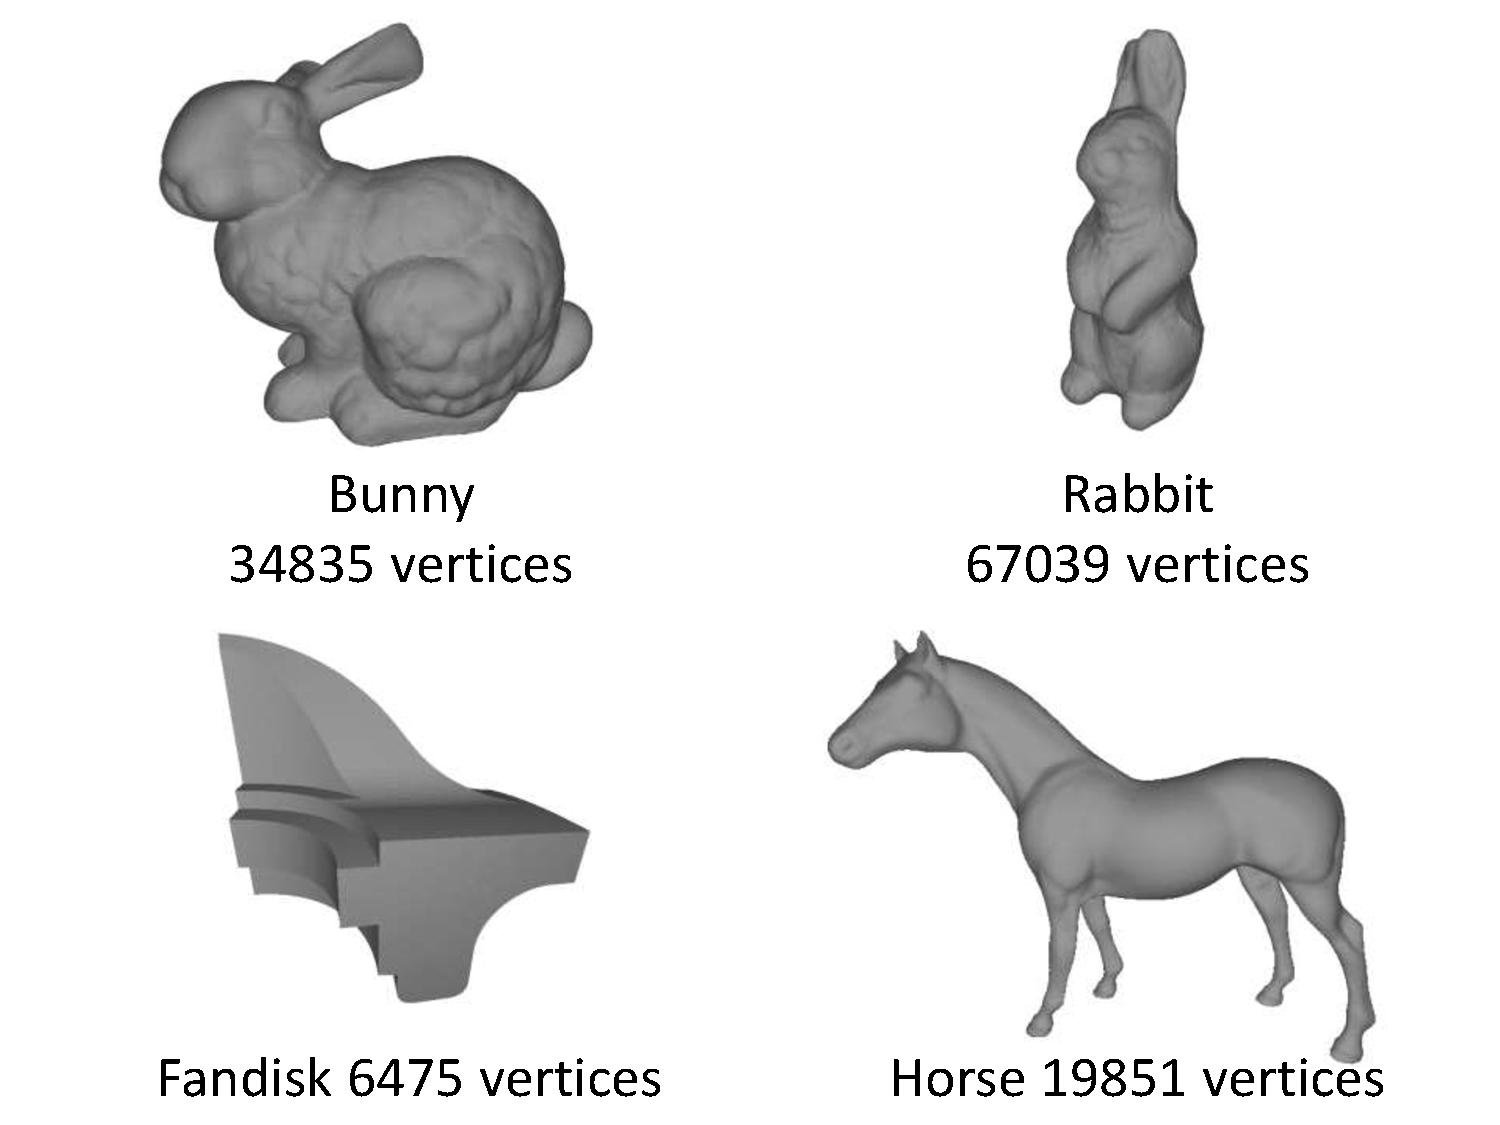
\includegraphics[width=4.0in]{images/experiments/test_data/modelsused}
\caption{Models used to assess the Plane-Tree compression algorithm.}
\label{fig:MODELSUSEDA}
\end{figure}


Next, the Plane-Tree is compared with the current state-of-the-art methods from 3D object compression research. These experiments are presented in section \ref{SEC:PTVSSOTA}. These experiments reveal that the Plane-Tree not only, outperforms the original octree method, but also some of the state-of-the-art transform methods at low-bit-rates. Several state-of-the-art algorithms are compared including some transform based methods \cite{Bayazit103DMesh,Khodakovsky00Progressive} and some compression systems which were designed to compress at low bit-rates \cite{Peng10Feature,Lincoln13Hons}. \\ 

To compare the Plane-Tree with each of these algorithms quantitatively, each algorithm is set-up to compress a model at different levels of compression vs quality. An algorithm's rate-distortion (RD) is plotted and compared to each of the other algorithms. Since lossy algorithms are compared, this indicates the amount of distortion (in the decoded model compared with the original) given a particular bit-rate. This measurement represents the number of bits each algorithm requires to store a particular model at a particular level of quality. The fewer bits required to represent a model of a given accuracy, the better the compression system performs. The mean error and root mean squared error discussed in section \ref{metricsSection} are used to measure the quality of the compressed models whilst the bit-rate in bits per vertex metric is used to measure the number of bits required to store the compressed model. Both the mean error and the root mean squared error are scaled by the main diagonal of the input model to make the results invariant to model size. Qualitative results comparing the Plane-Tree with other state-of-the-art methods are also presented. \\




%\section{Test Data}
%\label{TestDataSection}
%
In order to compare and analyse the FVR method as well as the MVVR and FVR-3D extensions, several real world data were captured for testing purposes. To analyse the robustness of the FVR method in terms of camera translation and rotation an indoor environment was captured using the Asus Xtion PRO live active camera. The results and descriptions for these experiments are shown in sections \ref{Sec:CamTransTrackExp} and \ref{Sec:CamRoteTrackExp}. This indoor environment contained several boxes and pieces of furniture. Therefore the data provide a useful and challenging but robust test for this 3D reconstruction method. The robustness of the FVR method in situations where moving objects impact registration is measured. Several 3D frames were captured for this experiment. These frames are captured from an indoor scene where furniture of different sizes are removed and added between frames. \\

Three scenes were captured in order to test the FVR method's qualitative performance. These scenes include the apartment scene, office scene and the garden scene. All three scenes were captured using the Asus XTION PRO live active camera at 30 frames per second. For each scene, only one in every 30 frames were registered, constituting real time FVR performance. The apartment scene was generated by moving and rotating the camera around an apartment living room before moving towards the kitchen area. This scene contains an abundance of features and would be considered a basic test for most 3D reconstruction algorithms. The second scene is the Office scene. This scene was generated by rotating the camera whilst zooming in and out on different objects within the room. Again this scene was reconstructed by registering every 30th frame. Despite both of the scenes being trivial to reconstruct, most algorithms (especially feature matching based methods) would find registering large rotations (such as those present in this data) difficult. The Garden scene is a difficult scene to reconstruct regardless of the reconstruction algorithm or technique used for registration. This scene was captured by rotating the camera around a garden outside the university. The scene contains many textures which are similar at the local level but are located in totally different locations. Therefore the scene is difficult to reconstruct using local and feature based methods such as FM+RANSAC and ICP. \\

The MVVR method was analysed using test data generated using a Microsoft passive RGB camera. The data output is in basic video format, and all depth information was generated implicitly by the MVVR algorithm. This data was captured by moving the camera whilst focusing on a set of textured boxes within an indoor environment. Several frames were captured at 30 frames per second and registered for analysis of the MVVR method qualitatively. Quantitative tests of the MVVR make use of the same data as tests for the FVR method (testing translation and rotational registration error). \\

Test data was also generated in order to robustly test and compare the FVR series of methods proposed in this research with different pose-estimation procedures and 3D registration methods in a variety of different scenes and settings each with features which push the boundaries for reconstruction in some way. Scenes which are both in-door and out-door were chosen for testing in order to measure the robustness and accuracy of these methods in both settings. Some scenes include large amounts of texture whilst others have little or no texture. Scenes with little texture are difficult for both SLAM and 3D reconstruction techniques because of the small amount of usable data by which a registration may be computed. Some scenes in the data-set were captured purposefully to measure the accuracy of these algorithms when large amounts of local features are identical within the scene. These scenes may confuse local methods because they contain multiple items/features/image patches which look similar locally but are actually different parts of possibly different objects within the scene, each having a unique global position which may be distant from that of another similar feature. Such scenes include carpet, plant-life, grass and generic plane walls or tiles. \\

This test-data also measures the accuracy, robustness and usefulness of each algorithm to register camera movements of different types. Each scene is captured with the camera performing certain an often singular type of movement. By testing with different movements, future algorithms may be constructed by switching to different registration methods based on camera movement. The different camera transformations recorded in the test data include: translation (left and right), zooming (and moving forward/backward) and rotation about different axes (x and y axis). \\

Some frames from these test videos are shown in appendix \ref{AppendixA}. The first scene: the Apartment Texture Rotate scene was taken by rotating the camera around the y-axis across an apartment. This scene contains a lot of texture information. The Apartment Texture X Axis scene is similar in terms of texture but contains both x and y axis rotation. This tests the FVR's ability to handle multiple axes of rotation. \\


The boxes scene was captured under arbitrary-rotation, translation and zoom (in/out) camera motions. It contains some useful information on the boxes themselves, however the texture on the carpet may cause texture confusion for feature based registration methods. The Desk Texture Translation scene contains a desk with a desktop computer and several items on it. The In-door space with texture-confusion contains a set of chairs and picture frames which look similar to each-other locally but may cause confusion for registration techniques which rely on local features. \\

The kitchen scene was captured with both translation and zoom camera movements. It contains very little texture with most of the scene containing a plain/flat white textured surface. The Office textured blind-spot rotation scene is a textured office scene where the camera is rotated about the y-axis. The scene is focused on a large divider which separates two desks. The divider may confuse registration methods which rely too heavily on minimization by aligning the large divider as a priority rather than taking into account the smaller details within the scene. An example of such an algorithm would be ICP and its derivatives. \\

The Office scenes contain a plenty of usable texture and different sets were created by translating, rotating about the y-axis and rotating about the x-axis. Other office scenes, where the camera captures objects in both the foreground and the background and where the camera is lifted and rotated whilst focussed on an office desk and chair combo. Some out-door scenes were also captured around the university. They are captured with both rotation and translation camera movements and are also labelled as being susceptible to texture confusion. \\

\section{Tools}
\label{ToolsSection}

In the experiments, various machines, devices and software were used to generate and perform tests. This equipment is discussed here. All experiments were performed on two machines. One is an Asus laptop running both Windows 10 and Ubuntu 16. This laptop has an Intel i7 CPU and an NVIDIA GeForce 840 M GPU with 4 GB of RAM. The other is a Dell desktop computer running Windows 7. This machine has an Intel i5 CPU and 4 GB of RAM. Both operating systems were chosen for convenience, the laptop with the GPU was chosen because it had a programmable GPU available on-board. \\ 

Both the Visual Studio C/C++ compiler on Windows and the GCC C/C++ compiler on Ubuntu were used to write programs for testing purposes. C++ version 17 was primarily used to write programs. C/C++ was chosen due to its known computational performance. Libraries used include: the OPEN-CV 3 computer vision library used for capturing, writing and processing image data, and CUDA used for writing General Purpose GPU (GPGPU) programs. OPEN-CV was chosen due to its extensive image processing functions and CUDA was chosen because it had powerful features suitable for GPU processing as well as an efficient 3D FFT method. Both Visual Studio (12 and 15) and Code Blocks 16 were used to write programs using the libraries and compilers. Both of these were chosen as the best compiler for the given OS. The METRO 3D object comparison tool was used for comparing 3D objects in Plane-Tree experiments. METRO was chosen to be a fair comparison tool to prevent bias. \\

To capture depth (RGB-D) video frames, the Asus Xtion Pro Live active camera was used to capture $640\times480$ video frames at 30 frames per second. This camera can capture depth between 0.8 and 3.5 m and was used to capture most of the test-data used in FVR experiments. This active camera was chosen because of its simplicity and accuracy as well as its compatibility with custom programming. \\ 

All source code and experiments are available online. The link for the FVR method is \url{https://github.com/lukes611/phdThesis} \href{https://github.com/lukes611/phdThesis}, and the link for the Plane-Tree source code is \url{https://github.com/lukes611/PlaneTree} \href{https://github.com/lukes611/PlaneTree}. Further discussion about the metrics used for testing these algorithms is given in section \ref{metricsSection}. \\  


\section{Error metrics}
\label{metricsSection}
In order to evaluate the accuracy of volume registration we use several error metrics including: Hausdorff error, mean squared error and the percentage of matched voxels. We describe mathematically those techniques here. All measurements are based on a simple function which computes the nearest neighbour for a given 3D point or voxel given a volume (or collection of 3D points). We define such a function, named nearest-neighbour in equation \ref{eqn:NN}.

\begin{equation} \label{eqn:NN}
NN(p, V) =  \{ q \in V | (Dist(q, p) < Dist(k, p))  \forall k \in V \}
\end{equation}

This function retrieves the closest corresponding point given a query point $p$ and a volume or point cloud of points, $V$. This function can be used to provide omni-directional error functions based on Hausdorff, mean squared and percentage accuracy error metrics.

Here some one-way error functions are described. The one was Hausdorff error is defined in \ref{eqn:HDOW} 

\begin{equation} \label{eqn:HDOW}
\sum_{k=0}^{N} Dist(P_k, NN(P_k, Q))
\end{equation}


%sota results
\section{Data Sources}
\label{Sec:FVRSOTA}
\subsection{Algorithms} 
\label{AlgorithmsSection}

In order to assess the FVR registration techniques further, other frame registration techniques used in the literature were implemented for comparative purposes. It is important to compare the FVR techniques with these methods because they represent the current standard in 3D reconstruction techniques. The technique which is thoroughly compared with the FVR methods is the 2D feature-matching + RANSAC based method. This method, discussed in section \ref{FMANDFM}, performs 2D feature matching to compare frames. Using these feature matches which correspond to 3D points within the projected depth maps, RANSAC is used to filter out outliers and iteratively estimate camera location and pose. This method is important to compare with the FVR techniques because it is still dominant within 3D reconstruction as well as in other areas of image processing and computer vision. Our experiments indicate that the FVR techniques outperform this 2D feature matching + RANSAC method whilst remaining closed form solutions which are often more robust in certain situations (such as reconstructing scenes with little texture or scenes where texture confusion is prevalent). Through empirical tests, SURF was chosen as the optimal 2D feature matching algorithm to use to compare with the FVR techniques. \\ 


In addition to comparisons with 2D feature matching + RANSAC, 3D feature matching + RANSAC (discussed in section \ref{Sec:3DFMMethod}) was also implemented and compared. In 2D feature matching, the features are found and matched between a pair of 2D-image frames and then RANSAC is used to compute camera pose. The camera pose is then used to reconstruct the scene. The 3D feature matching + RANSAC technique uses the same concept, but features are matched between the projected 3D frames rather than the 2D frames. The distinction between these approaches is that 2D feature matching is considerably faster, whilst 3D feature matching can handle wider baselines and takes into account certain spatial information which may give it an edge over the 2D feature matching approach, especially in scenes with less texture or repeated local textures (texture confusion). SIFT-3D was chosen as the 3D feature matching method of choice in comparing this technique with the FVR techniques. This decision was made based on empirical testing. \\

The Iterative Closest Point algorithm (discussed in section \ref{ICPSection}) is another technique which has dominated 3D reconstruction and SLAM research. The ICP method works by iteratively refining a registration between two models based on each point's nearest neighbour. ICP is popular within both 3D reconstruction and SLAM research because of its accuracy and consistency, additionally it works well on most scene types. The major disadvantage of this method is that it gets stuck in local minima if there is too much noise, or too wide a base-line. In either of these cases, ICP fails to register frames. ICP is also known to fail in cases where too few features are present. \\

Another algorithm present in the experiments is the Principal Components Analysis (PCA) method. PCA is used to find the mean and principal components of multi-dimensional data. The PCA method used for registration purposes, uses the computed principal axes and mean to register two 3D frames. This method is useful for registration purposes as it works on wide-baselines, is fast and provides additional information about the scene (in the form of principal components and mean point). The downside  to this method is that it is very susceptible to noise and misaligned data. The presence of which makes the mean and secondary axes inaccurate and useless. The proposed FVR-3D method makes use of the primary axis information from PCA so it is important to compare the two to find out what improvements are made by FVR-3D over a vanilla PCA approach. \\

In order to test the FVR approaches (FVR discussed in section \ref{Sec:AFVRApproach} and FVR-3D discussed in section \ref{FullRecovery3DSection}), both algorithms are used to compute the registration between frames. The registration with the lowest error margin is used for comparisons with other methods, this combines the FVR accuracy with the FVR-3D's ability to register arbitrary 3D rotation. The combined FVR algorithm is proposed to handle general transformations in terms of rotation, scaling and translation whilst still being a closed form solution which is robust to large amounts of data noise, texture-confusion and scenes with a considerable lack of texture. This makes it a viable alternative in the 3D registration, 3D reconstruction and SLAM research areas. \\


\subsection{Sensor Types} 
\label{SensorTypesExpsSection}

Experiments show that the FVR based techniques are capable of registration across the three primary types of sensors used in 3D reconstruction and SLAM research. These sensors include stereo sensors, which are capable of generating dense depth data with the highest accuracy and resolution; active cameras, which are efficient hardware based solutions to depth generation; and monocular cameras, which produce the least accurate and most noisy depth maps. As mentioned in the literature review these sensor types have associated advantages and disadvantages. \\

The results from testing the stereo Kitti data set are presented in section \ref{StereoSOTA}. These results show that FVR based methods, particularly FVR-3D are suitable for dense 3D reconstruction and are highly robust to noise, object movement and outdoor scenes. In particular, it is shown that the FVR-3D method is capable of outperforming other algorithms used in the literature in terms of registration accuracy. Below is a list of data included in the Kitti Benchmark Dataset, data used in experiments are documented in the list. \\



\begin{easylist}[itemize]
\ListProperties(Space*=-1em,Space=-1em)
& Grayscale stereo images
&& Synced and Rectified
&& resolution: 1390 x 512
&& captured with a 0.5 mega-pixel camera
&& used in experiments
& RGB-Colour stereo images
&& Synced and Rectified
&& resolution: 1390 x 512
&& captured with a 0.5 mega-pixel camera
&& used in experiments
& 3D point clouds
&& generated using a Velodyne laser scanner
&& max depth: 120m
&& ~100,000 points per frame
&& stored as a list of float based vectors in binary format
&& used in experiments
& 3D GPS / IMU data
&& location, speed, acceleration and other meta-data information
&& text format
& Calibration Data 
&& Camera
&& Camera to GPU/IMU
&& Camera to Velodyne [used in experiments]
&& text file
& 3D object tracklet labels
&& cars, trucks, trams, pedestrians and cyclists
&& xml file
\end{easylist}


Section \ref{ActiveSOTA} presents the results of testing scenes captured using the Asus Xtion Pro Live active camera. Various types of scenes and camera movements were recorded and results show the FVR based methods perform robust and accurate 3D reconstruction. In particular, the FVR-3D can outperform other techniques from the literature, even when faced with a reduction in depth resolution when using the active camera as opposed to the stereo set-up tested with the Kitti Vision Benchmark data set. A list of data within this dataset is shown below.  \\

\begin{easylist}[itemize]
\ListProperties(Space*=-1em,Space=-1em)
& RGB-Colour images
&& Synced \& Calibrated
&& resolution: 640 x 480 (when calibrated), (1240 x 1080 max)
&& 30-60 frames per second
&& used in experiments
& 3D point clouds
&& generated using a structured light technique
&& depth range: 0.8m - 3.5m
&& low resolution: 640 x 480
&& 30 frames per second
&& used in experiments
& 3D GPS / IMU data
\end{easylist}


Lastly, section \ref{Sec:MonocularSOTA} presents the results of the MVVR method, the FVR extension for monocular sensor input data sets. Experiments revealed that the MVVR is not able to robustly handle rotation due to the noise generated when building the depth map, however, translation is possible. It can be said based on empirical results that the FVR based technique's accuracy and robustness increases with the resolution and accuracy of the depth maps used as input. Below is a list of data used in these experiments. \\

\begin{easylist}[itemize]
\ListProperties(Space*=-1em,Space=-1em)
& RGB-Colour images
&& Asus Xtion Pro Live camera
&&& resolution: 1240 x 1080
&&& 30 frames per second
&& Microsoft Life-Cam HD3000
&&& resolution: 1240 x 1080
&&& 30 frames per second
\end{easylist}



%stereo tests
\subsection{Stereo Camera}
\label{StereoSOTA}
	
In these experiments, several current techniques (2D Feature Matching (FM-2D), 3D Feature Matching (FM-3D), ICP and PCA) are compared to the FVR technique in terms of stereo camera registration accuracy. To this end, five data sets from the Kitti Vision Benchmark data set \cite{Geiger13Vision} were used. Each data set scene is a complicated outdoor environment filmed using an autonomous driving platform. The majority of frames contain moving objects which interfere with the registration process of several algorithms. \\

Each Kitti Vision Benchmark data set contains accurate laser scans, stereo grey-scale images, stereo RGB-images and GPS and IMU data. To simulate the theoretical situation in which stereo cameras generate the most accurate depth maps, the laser scans are used in place of depth data computed by a stereo disparity algorithm. Therefore, in these experiments, only the laser scans and stereo colour and greyscale images are used. \\

The five stereo data sets used in the experiments are shown in Figures \ref{fig:KT1DSS}, \ref{fig:KT2DSS}, \ref{fig:KT5DSS}, \ref{fig:KT91DSS} and \ref{fig:KT95DSS}. The first scene is the Kitti 0001 Sync Data Set, this scene has 107 frames. This data set contains 12 cars, two cyclists and a tram. The tram and cyclists are non-static objects within the scene, making it more difficult for the current set of reconstruction algorithms which rely on scenes being primarily static in nature. To the right in this data set, there is a tram-line and some trees and gardens, to the left is a residential street. The second scene is the Kitti 0002 Sync data set, this set is 76 frames long. It contains one car and two cyclists which are non-static objects. Within this scene there is a long brick wall hiding some tall trees, several cyclists ride along next to the wall. To the left, there are some grassy areas, some buildings and some parked cars. \\

At 153 frames, the Kitti 0005 Sync data set is also used. This scene contains nine cars, three vans, two pedestrians and one cyclist. Because of the size of the van and the other non-static objects within the scene, this appears to be one of the more difficult scenes to register. The camera winds through several different streets as opposed to the previous data sets which are mostly of one long road. The fourth data set used, the Kitti 0091 Sync data set is composed of 339 frames making it the largest data set used in these experiments. This data set contains two cars, a van, 42 pedestrians, 14 sitters, eight cyclists and one miscellaneous object. As it contains many non-static objects this scene is also considered difficult like the Kitti 0005 data set. \\

The last Kitti Vision Benchmark data set used is the Kitti 0095 data set. Unlike the previous data sets, all 267 frames only contain static objects, and the scenes are made up primarily of small winding streets. \\ 

Experiments are tabled in full at per frame intervals in Appendix \ref{StereoResultsRaw}. Here, registration errors are presented where frame $n$ is registered against frame $n+1$ and the registration error is reported for each algorithm. The error function used is the Mean Squared Error $MSE(P,Q)$. This error is computed between the consecutive frames after registration. This error value is computed as in equation \ref{eqn:msesota}. Here, the function $Register(x)$ is replaced by the registration method being tested. \\

\begin{equation} \label{eqn:msesota}
Error(frame_1, frame_2) =  \frac{Register(frame_1), frame2}{MSE(frame_1,frame_2)}
\end{equation}

\begin{figure*}[t]
\centering
\begin{subfigure}[b]{6.8cm}
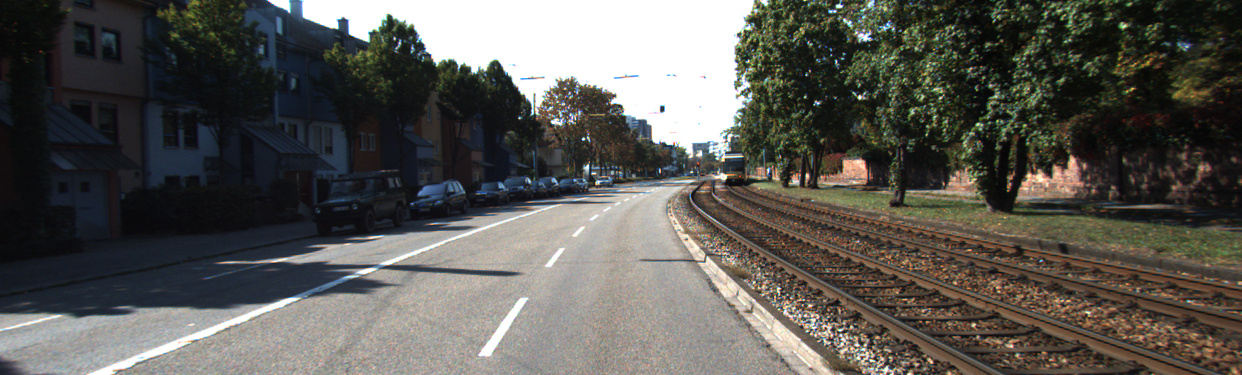
\includegraphics[width=6.5cm]{{images/experiments/stereo/1.1}.png}
\caption{Frame 1}
\end{subfigure}%
\begin{subfigure}[b]{6.8cm}
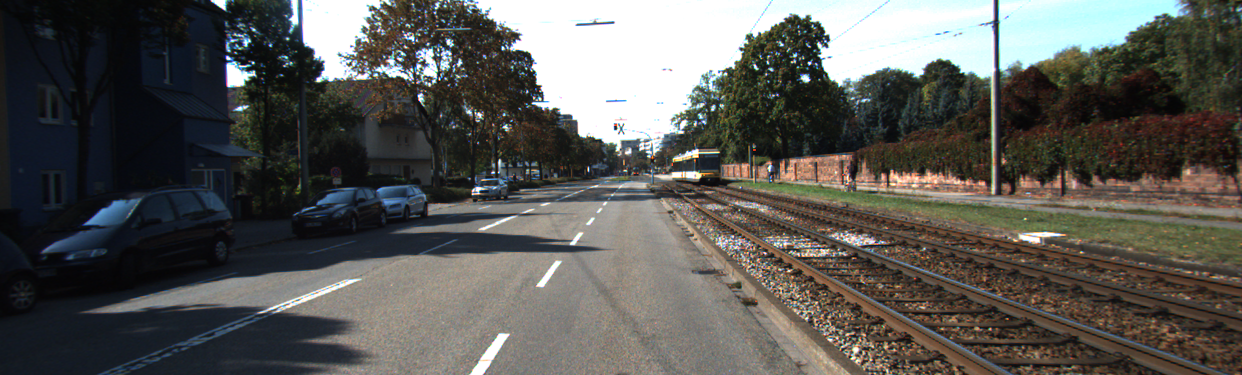
\includegraphics[width=6.5cm]{{images/experiments/stereo/1.2}.png}
\caption{Frame 39}
\end{subfigure}
\begin{subfigure}[b]{6.8cm}
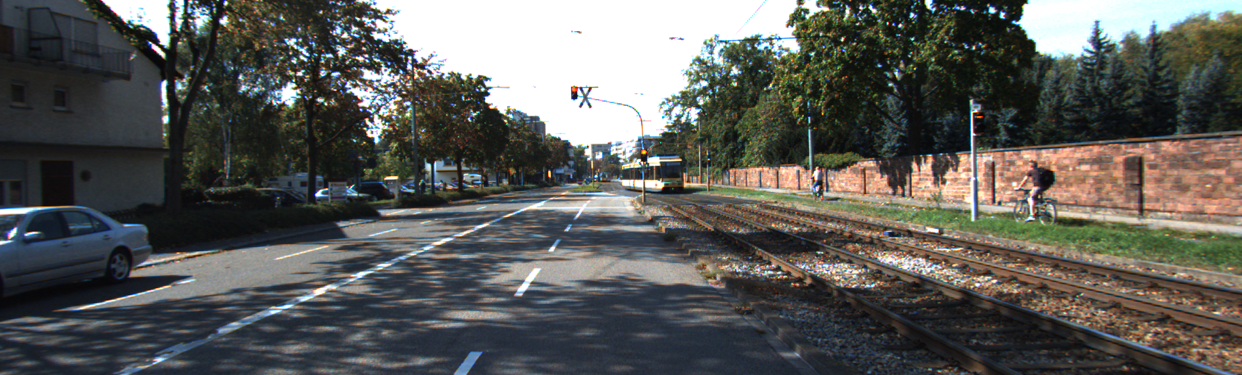
\includegraphics[width=6.5cm]{{images/experiments/stereo/1.3}.png}
\caption{Frame 77}
\end{subfigure}%
\begin{subfigure}[b]{6.8cm}
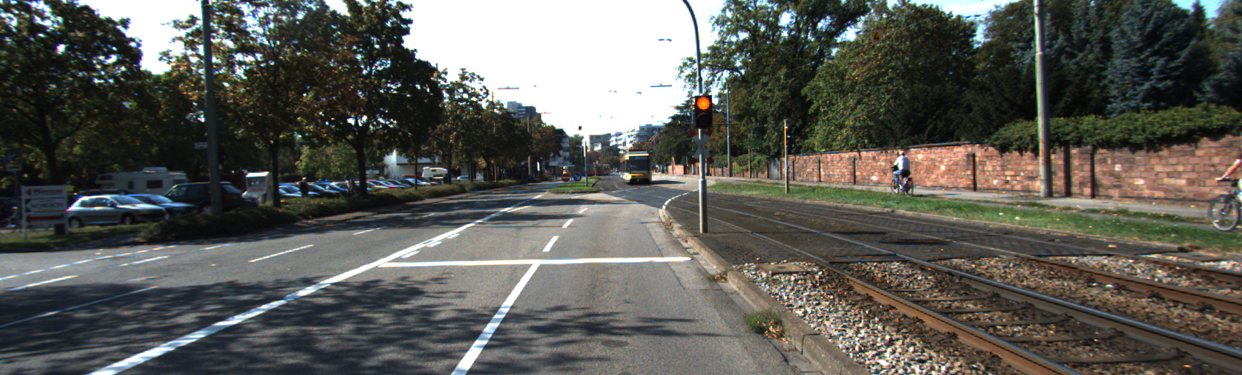
\includegraphics[width=6.5cm]{{images/experiments/stereo/1.4}.png}
\caption{Frame 114}
\end{subfigure}
\caption{Kitti 0001 Sync Data Set Sample}
\label{fig:KT1DSS}
\end{figure*}


The summary of these results is also tabled here for convenience. For each algorithm, the median registration error is provided. This is computed by listing and sorting the registration error values for a particular algorithm and selecting the value in the middle. Also included is the percent of best results metric. This measures in percentage, the frequency of times a particular algorithm achieved the best (lowest error) registration result compared to the other algorithms tested. An algorithm with a lower median error than another algorithm has performed better overall. Additionally, if an algorithm has a higher percentage of best results, it outperformed the other algorithms most of the time. If an algorithm achieved an average percentage of best results but a higher median error, this could be explained by outliers. If an algorithm achieved a lower median error but did not achieve the highest percentage of best results, it may be due to having a very competitive and consistent registration error. \\


Table \ref{tab:kittidata0001sync} presents results for the Kitti 0001 Sync data set, some example colour frames are shown in Figure \ref{fig:KT1DSS}. The road in which this scene was filmed contains a tram-line and moving tram as well as a garden area to the right and a line of parked cars and houses under cover of shadows to the left. Registration statistics were taken over the full length of this data set, which is 107 frames. Results show that FVR-3D achieved the lowest median registration error, ICP achieved the next lowest followed by FM2D and the FVR method. FVR-3D also achieved the highest percentage of best frame registration results at ~34.91 \% compared to ICP with ~27.36 \%. If the FVR methods were combined as a single hybrid method, they would have computed the best registration result 55.67 \% of the time. The FVR method alone outperformed FFVR, PCA and FM-3D. The FM-3D method (which had several frame registration failures, as is evident in its statistics) and the PCA method were the worst performers on this data set. The FFVR, whilst faster than the FVR method is slightly worse off in terms of performance. \\ 

%% sync 0001
\begin{table}[t]
\centering
\caption{Reconstruction Errors for the Kitti Data 0001 Sync Data Set}
\begin{tabular}{ccc}
\hline
\textbf{Algorithm} & \textbf{Median Error $\times$ 1000} & \textbf{\% best results}\\ \hline
FM2D	& 5.28 & 13.21\%\\
FM3D	& 9235.71 & 0.94\%\\
ICP	& 5.15 & 27.36\%\\
PCA	& 5.66 & 2.83\%\\
FVR	& 5.5 & 13.21\%\\
FFVR	& 5.59 & 7.55\%\\
FVR-3D	& 5.1 & 34.91\%\\
\end{tabular}
\label{tab:kittidata0001sync}
\end{table}








Table \ref{tab:kittidata0002sync} presents median error and percent best result statistics for the Kitti 0002 Sync Data Set, example colour frames are shown in Figure \ref{fig:KT2DSS}. The road in which this scene contains some parked cars to the left as well as a building, some grass and some large trees. To the right there is an orange brick wall and some trees and gardens as well as two moving cyclists. Results for the full 74 frames of the data set show that the FVR-3D method achieved the lowest median registration error at 4.27. The ICP algorithm achieved the next best result at 4.43 and the non-rotation-invariant FVR method achieved the third best result. Combined, the FVR based methods achieved the best result ~50.67 \% of the time compared to ICP at 30.67 \%. In this scene, the FM-3D method did not have as many registration failures and achieved a better result than the FFVR method and a comparable result to the PCA method. \\ 

%% sync 0002
\begin{table}[t]
\centering
\caption{Reconstruction Errors for the Kitti Data 0002 Sync Data Set}
\begin{tabular}{ccc}
\hline
\textbf{Algorithm} & \textbf{Median Error $\times$ 1000} & \textbf{\% best results}\\ \hline
FM2D	& 4.78 & 5.33\%\\
FM3D	& 4.85 & 6.67\%\\
ICP	& 4.43 & 30.67\%\\
PCA	& 4.86 & 6.67\%\\
FVR	& 4.67 & 6.67\%\\
FFVR	& 5.23 & 5.33\%\\
FVR-3D	& 4.27 & 38.67\%\\
\end{tabular}
\label{tab:kittidata0002sync}
\end{table} 



\begin{figure*}[t]
\centering
\begin{subfigure}[b]{6.8cm}
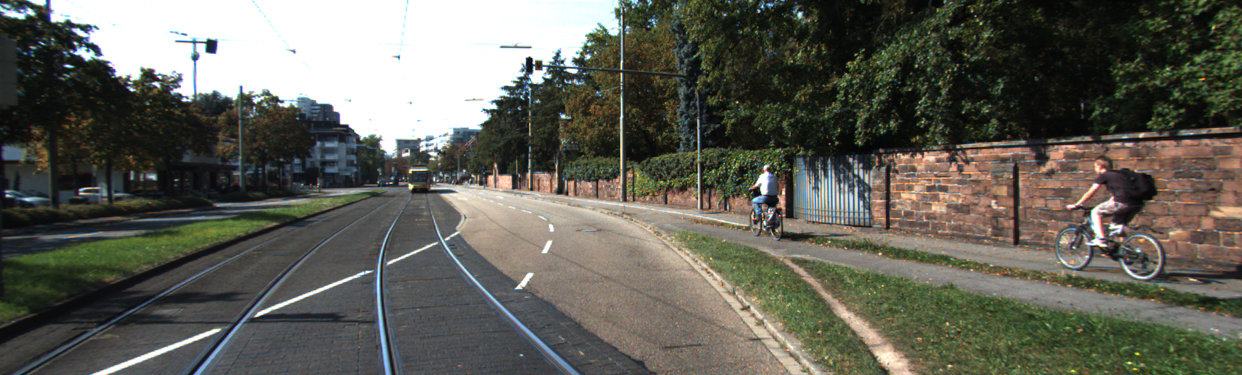
\includegraphics[width=6.5cm]{{images/experiments/stereo/2.1}.png}
\caption{Frame 1}
\end{subfigure}%
\begin{subfigure}[b]{6.8cm}
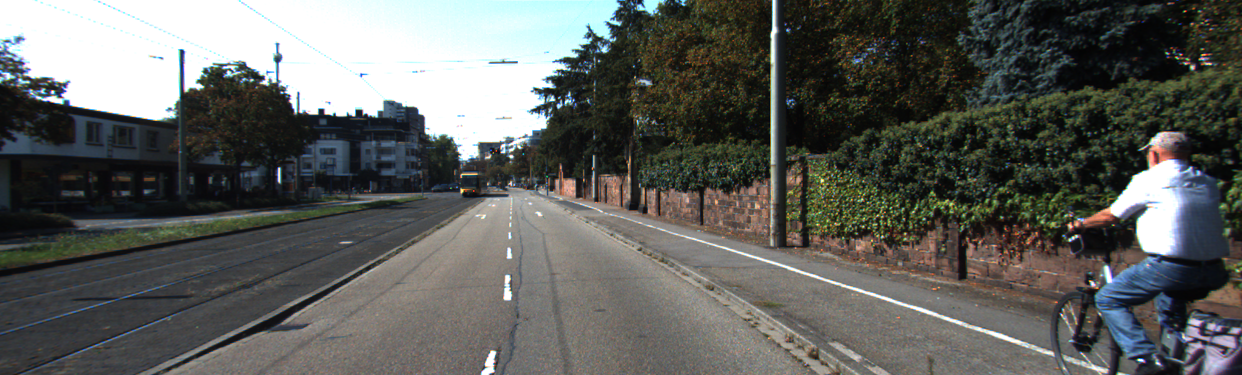
\includegraphics[width=6.5cm]{{images/experiments/stereo/2.2}.png}
\caption{Frame 28}
\end{subfigure}
\begin{subfigure}[b]{6.8cm}
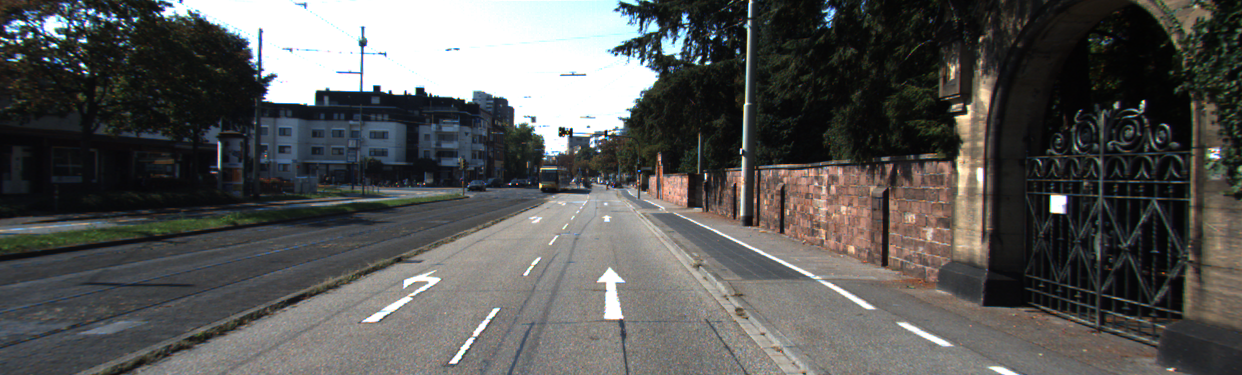
\includegraphics[width=6.5cm]{{images/experiments/stereo/2.3}.png}
\caption{Frame 56}
\end{subfigure}%
\begin{subfigure}[b]{6.8cm}
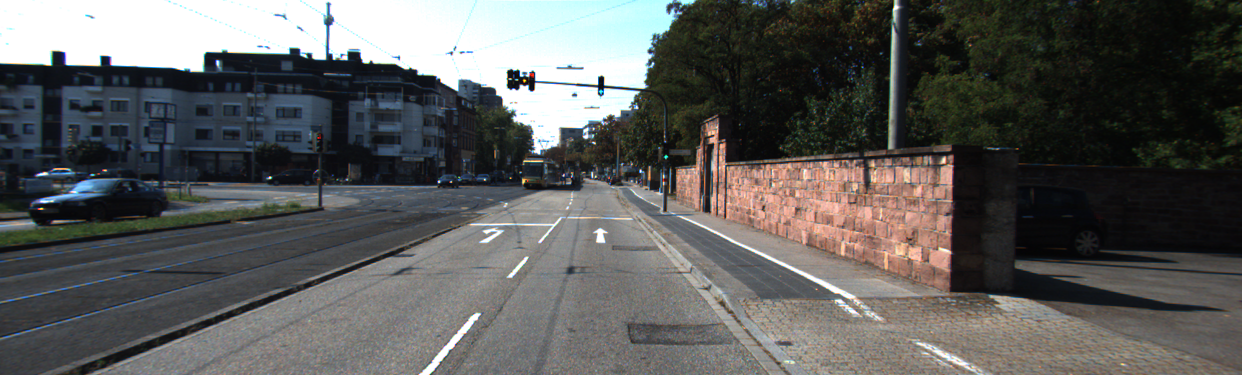
\includegraphics[width=6.5cm]{{images/experiments/stereo/2.4}.png}
\caption{Frame 83}
\end{subfigure}
\caption{Kitti 0002 Sync Data Set Sample}
\label{fig:KT2DSS}
\end{figure*}



 

Statistics for the Kitti 0005 Sync Data Set are presented in Table \ref{tab:kittidata0005sync}, example colour frames are shown in Figure \ref{fig:KT5DSS}. The scene captured in this data set was more difficult than previous scenes as it contains two moving cyclists and one large van which are all moving around in the scene without any relation to camera movement. In other words, these non-static objects cause major difficulties in most registration algorithms. In the full 152 frames of the data set, FM2D performed best with the lowest median error and highest percentage of best results. Next, FVR-3D also performed well with the second best median error and percentage of best results measurement. ICP achieved the third best median error and percentage of best results. In the results for this data set, FVR outperformed the FFVR method, as well as PCA and FM3D. Combined, the FVR algorithms achieved the best registration result 35.29 \% of the time, which is still below the performance of FM2D on this data set. \\

%% 0005
\begin{table}[t]
\centering
\caption{Reconstruction Errors for the Kitti Data 0005 Sync Data Set}
\begin{tabular}{ccc}
\hline
\textbf{Algorithm} & \textbf{Median Error $\times$ 1000} & \textbf{\% best results}\\ \hline
FM2D	& 3.39 & 39.22\%\\
FM3D	& 3.83 & 0\%\\
ICP	& 3.49 & 25.49\%\\
PCA	& 4.06 & 0\%\\
FVR	& 3.7 & 5.88\%\\
FFVR	& 4.25 & 1.96\%\\
FVR-3D	& 3.42 & 27.45\%\\
\end{tabular}
\label{tab:kittidata0005sync}
\end{table}

\begin{figure*}[t]
\centering
\begin{subfigure}[b]{6.8cm}
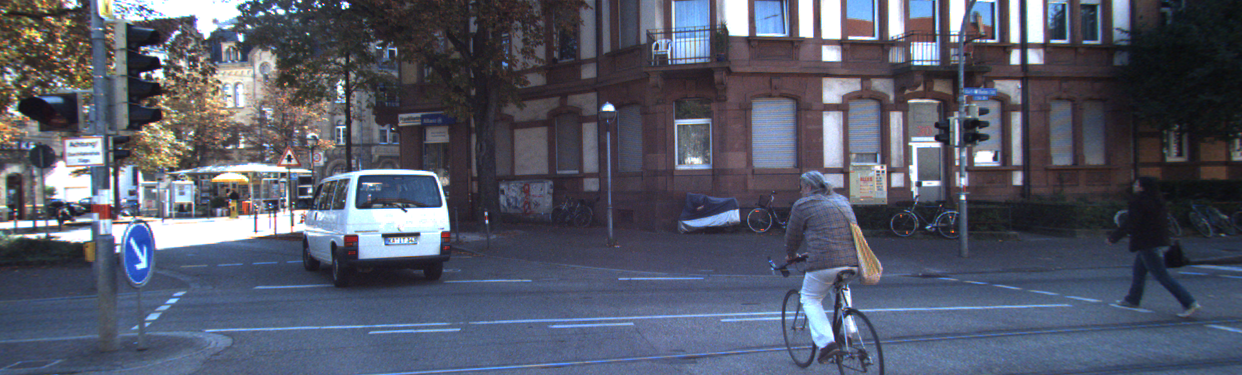
\includegraphics[width=6.5cm]{{images/experiments/stereo/5.1}.png}
\caption{Frame 1}
\end{subfigure}%
\begin{subfigure}[b]{6.8cm}
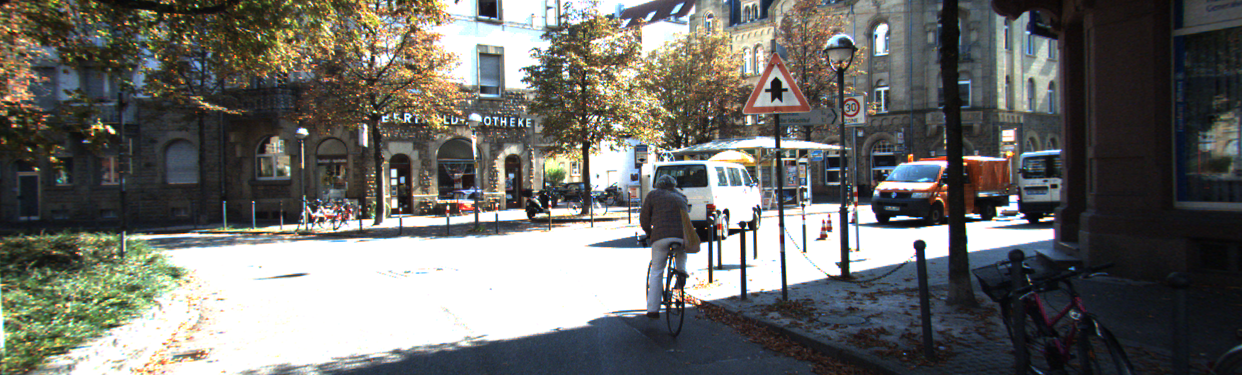
\includegraphics[width=6.5cm]{{images/experiments/stereo/5.2}.png}
\caption{Frame 54}
\end{subfigure}
\begin{subfigure}[b]{6.8cm}
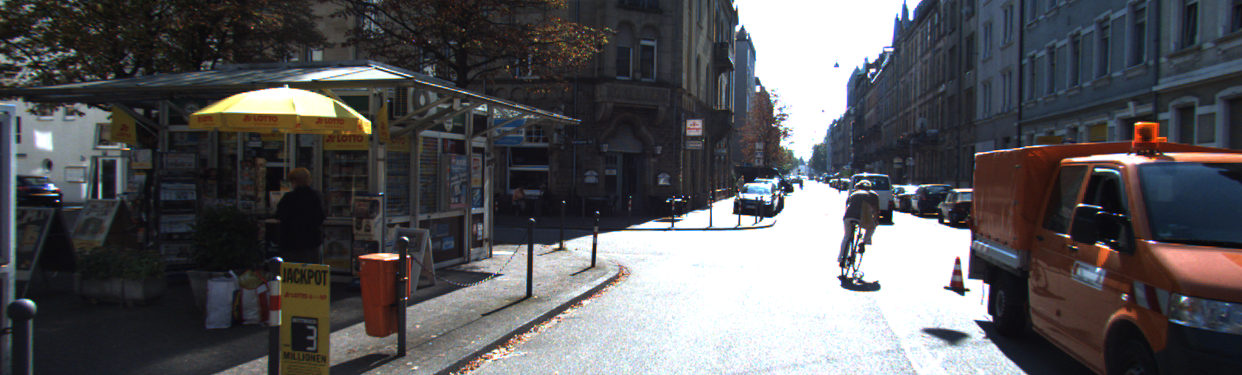
\includegraphics[width=6.5cm]{{images/experiments/stereo/5.3}.png}
\caption{Frame 107}
\end{subfigure}%
\begin{subfigure}[b]{6.8cm}
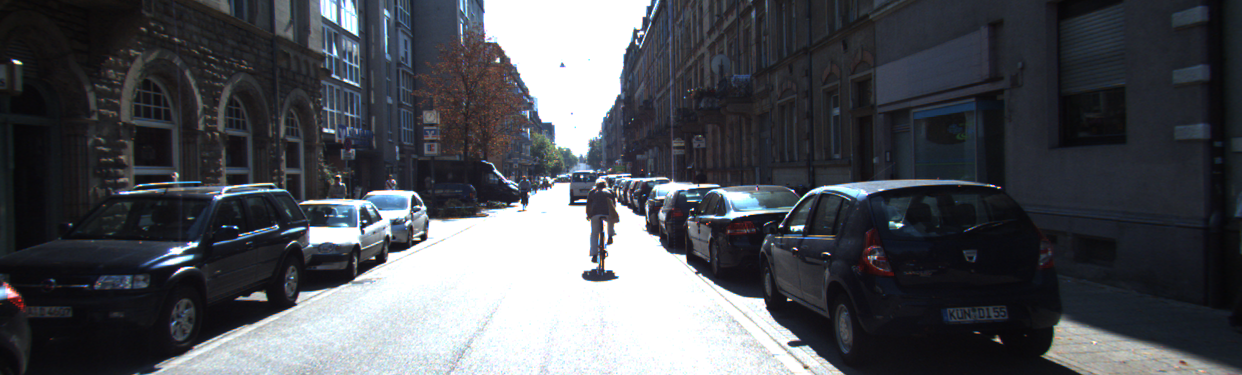
\includegraphics[width=6.5cm]{{images/experiments/stereo/5.4}.png}
\caption{Frame 160}
\end{subfigure}%
\caption{Kitti 0005 Sync Data Set Sample}
\label{fig:KT5DSS}
\end{figure*}



Table \ref{tab:kittidata0091sync} presents results for the Kitti 0091 Data Set, example colour frames from the data set are shown in Figure \ref{fig:KT91DSS}. This is the largest data set tested at 339 frames. The scene filmed in this data set is that of an outdoors inner city. It contains many moving agents making it a scene which is difficult to register for most registrations algorithms. Specifically, it contains two cars, a van, 42 pedestrians and eight cyclists. Registration results show FVR-3D outperformed all the other algorithms in terms of both median error and percentage of best results. The FVR algorithm achieved the next best results. The FVR-3D algorithm achieves the best result more than twice as often as ICP and FM2D. The FVR based methods performed well on this data set, a hybrid approach would have achieved the best results 65.19 \% of the time.  \\  	

%% kitti dataset 0091 Sync
\begin{table}[t]
\centering
\caption{Reconstruction Errors for the Kitti Data 0091 Sync Data Set}
\begin{tabular}{ccc}
\hline
\textbf{Algorithm} & \textbf{Median Error $\times$ 1000} & \textbf{\% best results}\\ \hline
FM2D	& 3.6 & 17.11\%\\
FM3D	& 4.04 & 0.88\%\\
ICP	& 3.61 & 15.63\%\\
PCA	& 4.1 & 1.18\%\\
FVR	& 3.57 & 20.94\%\\
FFVR	& 3.78 & 5.9\%\\
FVR-3D	& 3.43 & 38.35\%\\
\end{tabular}
\label{tab:kittidata0091sync}
\end{table} 


\begin{figure*}[t]
\centering
\begin{subfigure}[b]{6.8cm}
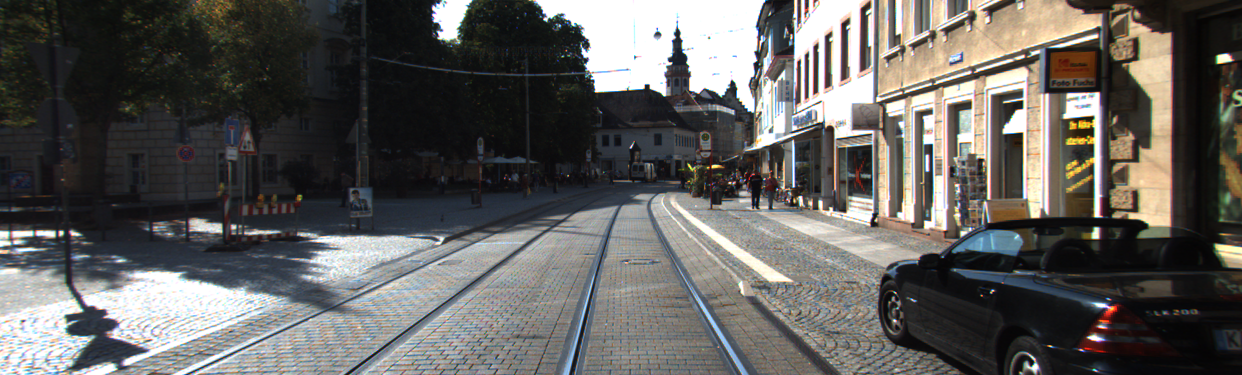
\includegraphics[width=6.5cm]{{images/experiments/stereo/91.1}.png}
\caption{Frame 1}
\end{subfigure}%
\begin{subfigure}[b]{6.8cm}
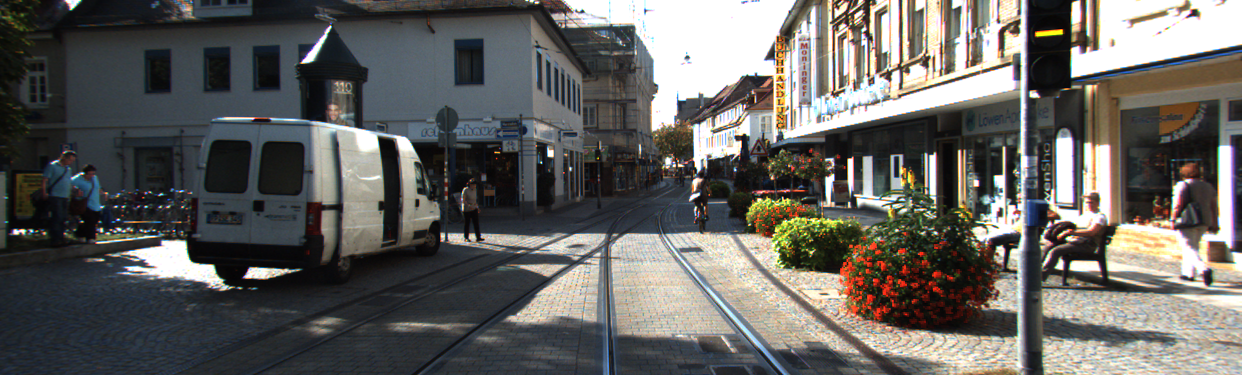
\includegraphics[width=6.5cm]{{images/experiments/stereo/91.2}.png}
\caption{Frame 116}
\end{subfigure}
\begin{subfigure}[b]{6.8cm}
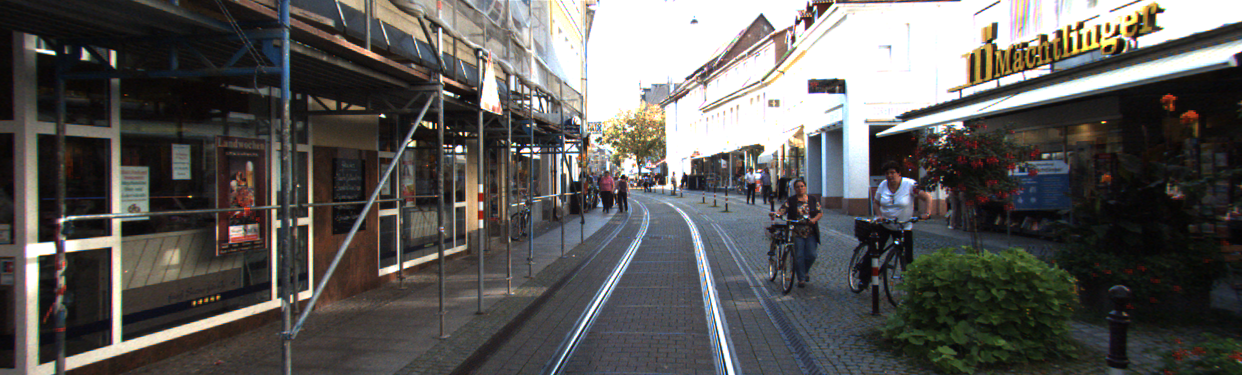
\includegraphics[width=6.5cm]{{images/experiments/stereo/91.3}.png}
\caption{Frame 231}
\end{subfigure}%
\begin{subfigure}[b]{6.8cm}
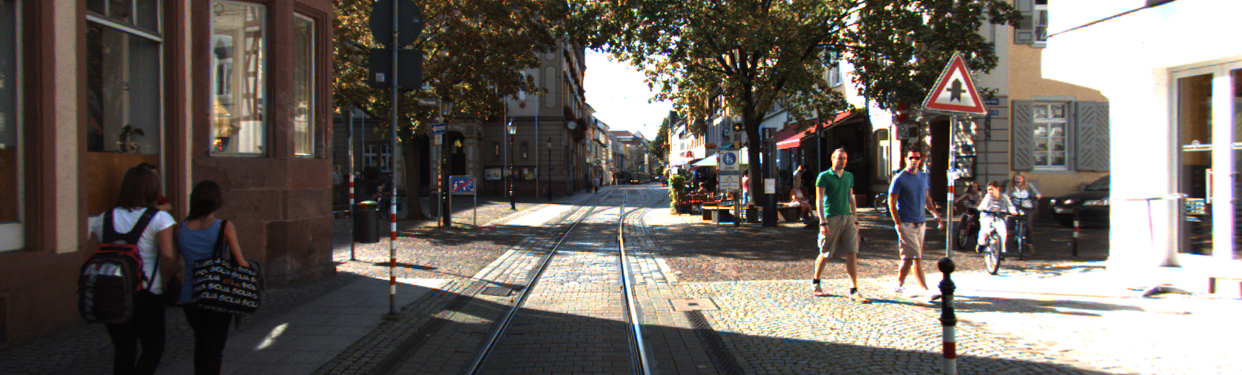
\includegraphics[width=6.5cm]{{images/experiments/stereo/91.4}.png}
\caption{Frame 346}
\end{subfigure}%
\caption{Kitti 0091 Sync Data Set Sample}
\label{fig:KT91DSS}
\end{figure*}



Results for the Kitti 00095 Data Set are presented in Table \ref{tab:kittidata0095sync} and Figure \ref{fig:KT95DSS} presents four example colour images from this data set. This scene was much more static than the previous scenes. It contains primarily parked cars and buildings in an inner-city environment. There are a few pedestrians and cyclists which are moving agents within the scene. This data set is 266 frames and results show that FVR-3D achieves both the best (lowest) median error score and the highest percentage of best results score at ~46.82 \%. The FVR algorithm achieved the second best results in terms of both the median error and percentage of best results metrics. ICP and FM2D were third and fourth, respectively. The FVR-3D algorithm achieved the best result three times more often than both the ICP and FM2D methods. \\

%% sync 0095
\begin{table}[t]
\centering
\caption{Reconstruction Errors for the Kitti Data 0095 Sync Data Set}
\begin{tabular}{ccc}
\hline
\textbf{Algorithm} & \textbf{Median Error $\times$ 1000} & \textbf{\% best results}\\ \hline
FM2D	& 4.19 & 12.36\%\\
FM3D	& 5.18 & 0\%\\
ICP	& 4.4 & 13.48\%\\
PCA	& 5.32 & 0.37\%\\
FVR	& 4.12 & 22.85\%\\
FFVR	& 4.73 & 4.12\%\\
FVR-3D	& 3.96 & 46.82\%\\
\end{tabular}
\label{tab:kittidata0095sync}
\end{table} 


\begin{figure*}[t]
\centering
\begin{subfigure}[b]{6.8cm}
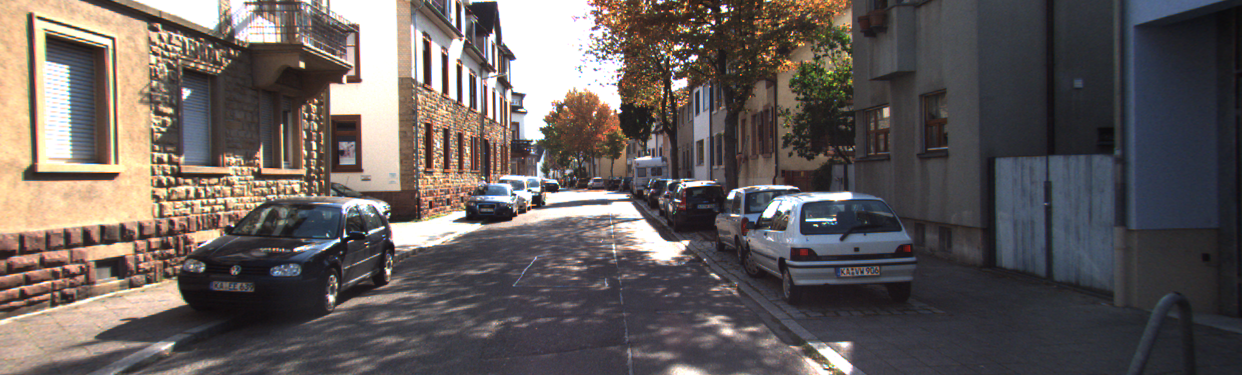
\includegraphics[width=6.5cm]{{images/experiments/stereo/95.1}.png}
\caption{Frame 1}
\end{subfigure}%
\begin{subfigure}[b]{6.8cm}
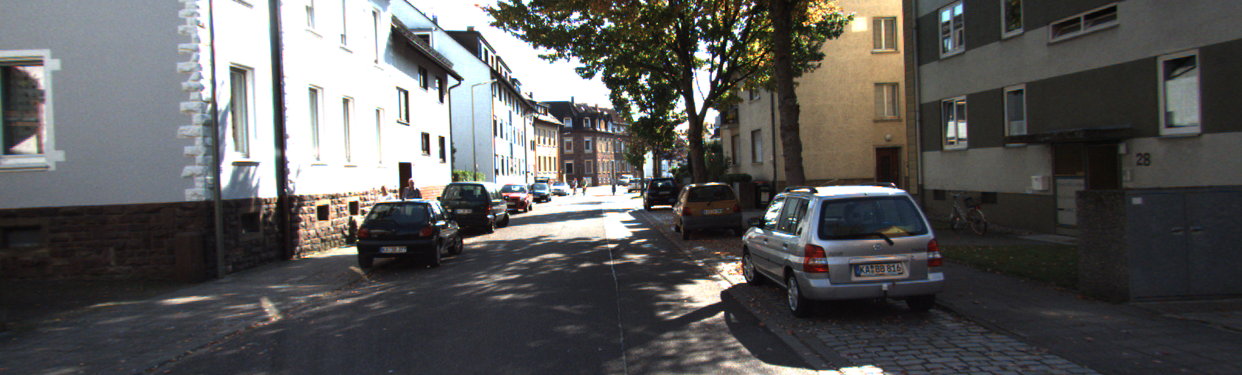
\includegraphics[width=6.5cm]{{images/experiments/stereo/95.2}.png}
\caption{Frame 92}
\end{subfigure}
\begin{subfigure}[b]{6.8cm}
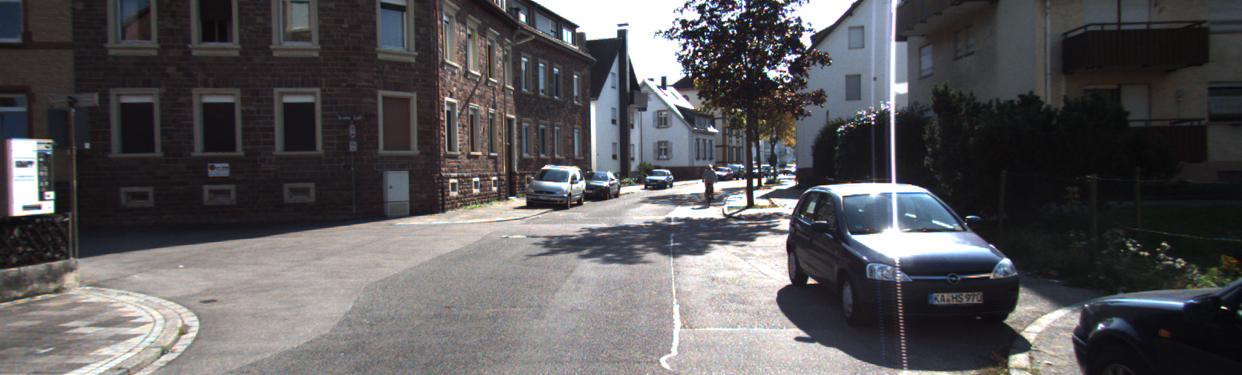
\includegraphics[width=6.5cm]{{images/experiments/stereo/95.3}.png}
\caption{Frame 183}
\end{subfigure}%
\begin{subfigure}[b]{6.8cm}
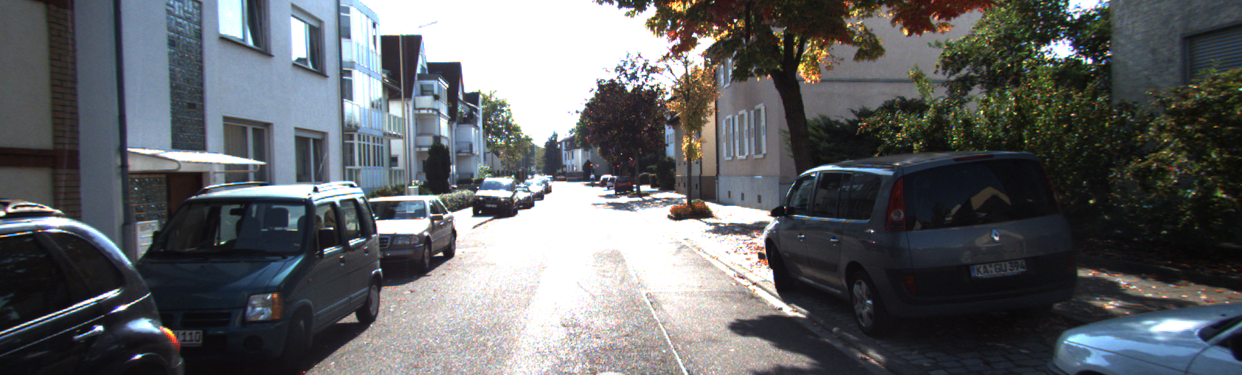
\includegraphics[width=6.5cm]{{images/experiments/stereo/95.4}.png}
\caption{Frame 274}
\end{subfigure}%
\caption{Kitti 0095 Sync Data Set Sample}
\label{fig:KT95DSS}
\end{figure*}


%active camera-tests
\subsection{Active Camera}
\label{ActiveSOTA}

Experiments evaluating the performance of the set of FVR related algorithms on active sensor camera input are presented here. These data-sets are all 25 frames long and captured of different environments using different camera movements. Due to the limitations of the ASUS Xtion PRO LIVE active camera used, indoor scenes were captured primarily. Similarly to the results presented in section \ref{StereoSOTA} statistics are presented for algorithms from the literature (FM2D, FM3D, ICP \& PCA) as well as FVR based algorithms (FVR, FFVR \& FVR-3D) in the form of the median registration error and the percentage of best results. 

%%Apartment Texture Rotate:
\begin{figure}
\centering
\begin{tabular}{ccc}
\hline
\textbf{Algorithm} & \textbf{Median Error $\times$ 1000} & \textbf{\% best results}\\ \hline
FM2D	& 2.13 & 36\%\\
FM3D	& 5.14 & 0\%\\
ICP	& 2.42 & 16\%\\
PCA	& 8.61 & 4\%\\
FVR	& 2.87 & 8\%\\
FFVR	& 2.7 & 8\%\\
FVR3D	& 2.05 & 28\%\\
\end{tabular}
\caption{Statistics for the Apartment Texture Rotate Data Set}
\label{tab:apartmenttexturerotate}
\end{figure} 



%%Apartment Texture X-Axis Rotation
\begin{figure}
\centering
\begin{tabular}{ccc}
\hline
\textbf{Algorithm} & \textbf{Median Error $\times$ 1000} & \textbf{\% best results}\\ \hline
FM2D	& 1.97 & 4\%\\
FM3D	& 2.58 & 0\%\\
ICP	& 1.78 & 36\%\\
PCA	& 3.81 & 0\%\\
FVR	& 1.99 & 4\%\\
FFVR	& 2.01 & 0\%\\
FVR3D	& 1.87 & 56\%\\
\end{tabular}
\caption{Statistics for the Apartment Texture X-Axis Rotation Data Set}
\label{tab:apartmenttexturex-axisrotation}
\end{figure} 


%% desk texture translation
\begin{figure}
\centering
\begin{tabular}{ccc}
\hline
\textbf{Algorithm} & \textbf{Median Error $\times$ 1000} & \textbf{\% best results}\\ \hline
FM2D	& 1.24 & 8\%\\
FM3D	& 2.48 & 12\%\\
ICP	& 1.59 & 28\%\\
PCA	& 1.51 & 4\%\\
FVR	& 1.16 & 16\%\\
FFVR	& 1.29 & 16\%\\
FVR3D	& 1.23 & 16\%\\
\end{tabular}
\caption{Statistics for the Desk Texture Translation Data Set}
\label{tab:desktexturetranslation}
\end{figure} 



%%Office Textured Blindspot Rotation
\begin{figure}
\centering
\begin{tabular}{ccc}
\hline
\textbf{Algorithm} & \textbf{Median Error $\times$ 1000} & \textbf{\% best results}\\ \hline
FM2D	& 1.39 & 24\%\\
FM3D	& 5.92 & 0\%\\
ICP	& 1.2 & 44\%\\
PCA	& 4.83 & 8\%\\
FVR	& 2.07 & 0\%\\
FFVR	& 2.92 & 0\%\\
FVR3D	& 1.1 & 24\%\\
\end{tabular}
\caption{Statistics for the Office Textured Blindspot Rotation Data Set}
\label{tab:officetexturedblindspotrotation}
\end{figure} 

%%Office Textured Items Translation
\begin{figure}
\centering
\begin{tabular}{ccc}
\hline
\textbf{Algorithm} & \textbf{Median Error $\times$ 1000} & \textbf{\% best results}\\ \hline
FM2D	& 2.89 & 24\%\\
FM3D	& 5.45 & 0\%\\
ICP	& 2.93 & 4\%\\
PCA	& 3.79 & 0\%\\
FVR	& 5.04 & 0\%\\
FFVR	& 3.06 & 28\%\\
FVR3D	& 2.83 & 44\%\\
\end{tabular}
\caption{Statistics for the Office Textured Items Translation Data Set}
\label{tab:officetextureditemstranslation}
\end{figure} 


%%office texture rotation
\begin{figure}
\centering
\begin{tabular}{ccc}
\hline
\textbf{Algorithm} & \textbf{Median Error $\times$ 1000} & \textbf{\% best results}\\ \hline
FM2D	& 4.36 & 26.92\%\\
FM3D	& 7.15 & 0\%\\
ICP	& 4.76 & 34.62\%\\
PCA	& 6.55 & 0\%\\
FVR	& 5.3 & 7.69\%\\
FFVR	& 4.74 & 7.69\%\\
FVR3D	& 4.35 & 23.08\%\\
\end{tabular}
\caption{Statistics for the Office Texture Rotation Data Set}
\label{tab:officetexturerotation}
\end{figure} 



%monocular-tests
\subsection{Monocular Camera}
\label{Sec:MonocularSOTA}

During experiments, it was found that MVVR (FVR applied to monocular camera sensor data) had considerably less accuracy and robustness than the other FVR methods (FVR, FFVR and FVR-3D). Additionally, we found that MVVR was less robust to rotational transforms. This is due to the fact that depth maps produced by monocular sensor methods, such as optical flow, do not produce sufficiently accurate and reliable depth maps. Results from stereo and active camera tests suggest that this is due to the reduction in accurate and precise depth data generation. \\

Nevertheless, to evaluate the performance of the MVVR method, quantitative experiments were performed on the Kitti Vision Benchmark Data Set. In these experiments, the MVVR method was compared with methods from the literature including FM2D, FM3D. ICP and PCA. Each depth map was projected into volume sizes of $256^3$ for processing by the rest of the MVVR method (the FVR part). To generate the depth maps, a local 2D block matching method was used. Kernel sizes used in the correlation procedure were $3 \times 3$ in size with a search area size of $21 \times 21$. The sizes of the kernel, search area and volume sizes were all chosen empirically. \\

Depth maps computed using the block matching method are only estimates of true scene depth. Therefore, resulting projections are not accurate. These projections, however, are still good enough to produce reconstructions. Registration of these inaccurate projections is difficult due to the amount of noise in the data. Figure \ref{fig:lidarVSMono} shows the noise contrast between depth maps produced by a LIDAR and a monocular block-matching system. \\

\begin{figure}[!htb]
\centering
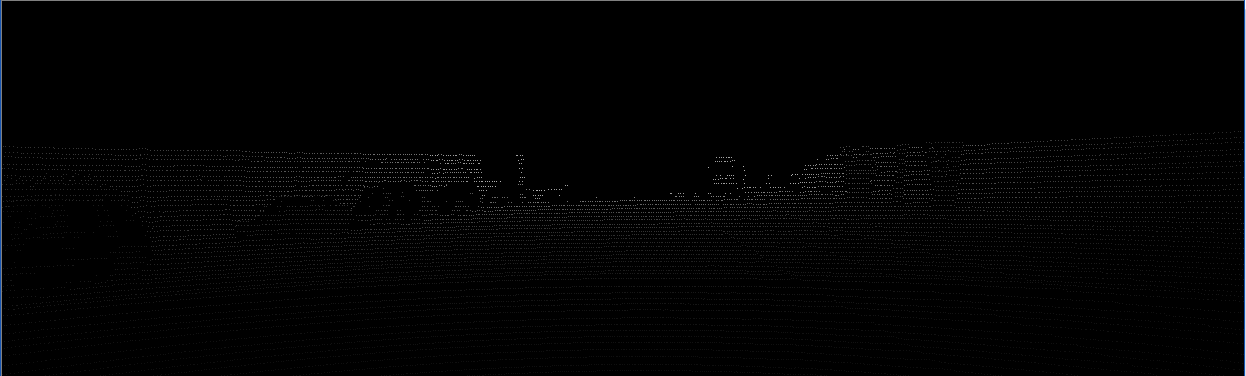
\includegraphics[width=2.9in]{images/methodology/FVR/mono/color}

\includegraphics[width=2.9in]{images/methodology/FVR/mono/depth}
\caption{Left: Ground Truth Depth Map Computed Using a LIDAR System, Right: Depth Map Computed Using a Monocular Method}
\label{fig:lidarVSMono}
\end{figure}


Results on the Kitti Benchmark 0001 Sync data set are shown in Table \ref{table:MVVRQuantitativeExperimentResults}. In these results, ICP outperformed the other methods, with each algorithm having larger errors due to the inaccurate depth maps. Here, FVR achieved the best result ~29.25 \% of the time. Compared to results in Table \ref{tab:kittidata0001sync}, the MVVR method was less competitive than ICP. Due to the low-quality projections, FM2D and PCA failed were not able to register every frame. Most of the algorithms had incorrectly registered frames at some point.

\begin{table}[t]
\centering
\caption{Reconstruction Errors for the Kitti Data 0001 Sync Data Set Using Monocular (RGB) Input Only}
\begin{tabular}{ccc}
\hline
\textbf{Algorithm} & \textbf{Median Error $\times$ 1000} & \textbf{\% best results}\\ \hline
FM2D	& 3742.4 & 2.83\%\\
FM3D	& 918.05 & 14.15\%\\
ICP	& 772.48 & 50.94\%\\
PCA	& 2046.96 & 2.83\%\\
MVVR	& 944.81 & 29.25\%\\
\end{tabular}
\label{table:MVVRQuantitativeExperimentResults}
\end{table} 

These results, and those from the Stereo and Active camera experiments, indicate that, if the quality of the depth maps had been higher, the FVR based methods would have produced better results. \\


%the basic tracking stuff
\section{Camera Tracking \& Noise Robustness}
\label{Sec:CamTransTrackExp}
\section{Camera Translation Tracking}
\label{Sec:CamTransTrackExp}

Experiments measuring the difference between the ground-truth camera movement and the registered camera movement using the FVR method are presented in this section. For these experiments, one camera frame of an office environment was captured using the ASUS Xtion PRO LIVE active camera. The camera was then moved (translated) by different amounts including: 5 centimeters, 10 centimeters and 15 centimeters. These distances were measured using a measuring tool, and a second frame was then captured. The FVR method was used to register both frames in order to measure the camera location separation between the frames. \\

Different levels of noise were added to both frames prior to 3D registration in order to measure the FVR registration method's ability to register frames with large amounts of noise. The Signal to Noise Ratio (SNR) metric is used to describe the noise added to both captured frames, prior to any registration. This noise effects any registration method's ability to accurately estimate the transformation separating two sets of data. A noise range value of $x$\% means random noise was added in the range [$\frac{-x}{2}$, $\frac{x}{2}$]. Camera registration error is measured in both centimetres (cm) and voxel error (the error in the phase correlation volume without taking into account the effects of quantization). Table \ref{table:trans} shows the results of these tests, they illustrate the FVR's robustness to noise whilst registering frames which are captured during different camera translation intervals. \\



%translation
\begin{table}[!htb]
\centering
\scalebox{1.0}{
\begin{tabular}{ccccc}
\hline
\textbf{translation (cm)} & \textbf{noise range (\%)} & \textbf{SNR} & \textbf{error (cm)} & \textbf{error (voxel)}\\ \hline
5cm & 0 & $\infty$ & 0 & 0\\
5cm & 10 & 20db & 0 & 0\\
5cm & 25 & 12db & 0 & 0\\
5cm & 50 & 6db & 0 & 0\\
5cm & 75 & 2.5db & 112.28 & 89.83\\
10cm & 0 & $\infty$ & 0 & 0\\
10cm & 10 & 20db & 0 & 0\\
10cm & 25 & 12db & 0 & 0\\
10cm & 50 & 6db & 156.65 & 125.32\\
15cm & 0 & $\infty$ & 2.8 & 2.24\\
15cm & 10 & 20db & 2.8 & 2.24\\
15cm & 25 & 12db & 2.8 & 2.24\\
15cm & 50 & 6db & 198.55 & 158.84\\
\\
\end{tabular}}
\\
\caption{Translation Tracking}
\label{table:trans}
\end{table}

Results show that the FVR method is accurately able to register frames up to 15 centimeters apart and for camera movements below 5 centimeters per frame, the FVR method can accurately register them. Results also indicate that, for these camera movements the FVR method can handle up to 75\% noise within the frame, which is a Signal to Noise (SNR) ratio of as little as 2.5 decibels. \\

It can be shown that the registration of camera movements using the FVR can handle movements up to 15cm as long as the SNR is higher than or equal to 6.0, meaning the FVR method is highly robust to noise. To put these camera translations into perspective at video frame rates, a displacement of 10 centimeters per frame equates to camera velocity of 3 meters per second which is about twice the normal walking speed. This is suitable for a majority of applications. \\


\section{Camera Rotation Tracking}
\label{Sec:CamRoteTrackExp}

Table \ref{table:rote} shows results for camera rotation experiments. The experiments, also captured with the ASUS Xtion PRO LIVE active camera, were created by capturing the first frame befroe rotating the camera about the y-axis by a number of degrees. The degrees were measured between rotations. Degrees of separation tested include: 10, 20 and 30 degrees. \\

Again, different levels of noise were added to both frames prior to registration. This experiment was designed to test the robustness of the FVR method in registering camera pose. The scene captured was the same office environment used in the translation experiment from section \ref{Sec:CamTransTrackExp}. \\

\begin{table}[!htb]
\centering
\scalebox{1.0}{
\begin{tabular}{ccccc}
\hline
\textbf{rotation} & \textbf{noise (\%)} & \textbf{SNR} & \textbf{error ($\theta$)} & \textbf{error (voxel)}\\ \hline
$10^{\circ}$ & 0 & $\infty$ & 0.31 & 0\\
$10^{\circ}$ & 10 & 20db & 0.31 & 0\\
$10^{\circ}$ & 25 & 12db & 0.63 & 1\\
$10^{\circ}$ & 30 & 10.5db & 90.62 & 96\\
$20^{\circ}$ & 0 & $\infty$ & 0.31 & 0\\
$20^{\circ}$ & 10 & 20db & 0.63 & 1\\
$20^{\circ}$ & 15 & 16.5db & 38.13 & 40\\
$30^{\circ}$ & 0 & $\infty$ & 3.75 & 4\\
$30^{\circ}$ & 10 & 20db & 3.28 & 3\\
$30^{\circ}$ & 15 & 16.5db & 30 & 32\\
\\
\end{tabular}}
\\
\caption{Rotation Tracking}
\label{table:rote}
\end{table}

Twelve degrees per frame is almost a full rotation per second in video rates. This is so fast that most cameras would acquire too much motion blur for registration to be possible. Therefore this test indicates the robustness of the FVR method within the context of camera pose estimation. \\

Given 10 degrees of separation, the error was below 1 degree for noise levels less than or equal to 30\%. This base line error is due to the sampling resolution of the volume, as voxel error was in fact zero. This metric removes the error which is primarily due to quantization noise. As with the translation experiments, the effect of noise increases with camera disparity. At 30 degrees of camera rotation, little matching information is available in order to perform a registration for most techniques. However, for noise levels of 10\% or less, voxel distance error was as low as 4 with an angular error less than $3.8$ degrees. As mentioned, rotations of this magnitude are unlikely as motion blur would occur. Therefore these results show both the effectiveness of the FVR in terms of pose registration, as well as robustness to noise interference. \\


\section{Object Motion Experiments}
\label{Sec:FVRMotionExp}

\begin{table}[!htb]
\centering
\scalebox{1.0}{
\begin{tabular}{ccc}
\hline
\textbf{Object Size} & \textbf{error (cm)} & \textbf{error (voxel)}\\ \hline
0.35 & 0 & 0\\
2.95 & 0 & 0\\
6.22 & 0 & 0\\
12.28 & 0 & 0\\
19.82 & 0 & 0\\
22.39 & 0 & 0\\
26.09 & 0 & 0\\
31.00 & 0 & 0\\
48.23 & 38.42 & 15\\
74.32 & 113.57 & 44\\
\\
\end{tabular}}
\\
\caption{Object Motion Test}
\label{table:OBJECT_MOVE_EXP}
\end{table}


In order to assess robustness to object motion, experiments were conducted by moving the ASUS Xtion PRO LIVE active camera backwards along the z-axis by 5 centimeters per frame whilst moving objects were placed in and out of the scene so that they only appear in one of the volumes being registered. Various sized objects including stacks of CDs, large boxes, people and several pieces of furniture were used and are measured by the percentage of the frame they occupy. Results from table \ref{table:OBJECT_MOVE_EXP} show the proposed method was accurate upto an object size of 31\%, but failed for objects taking up over 48.23\%.

\section{Reconstructed Scenes}
\label{Sec:FVRQual1Exp}

\begin{figure}[!htb] 
        \centering
        \begin{subfigure}[b]{3.0in}
                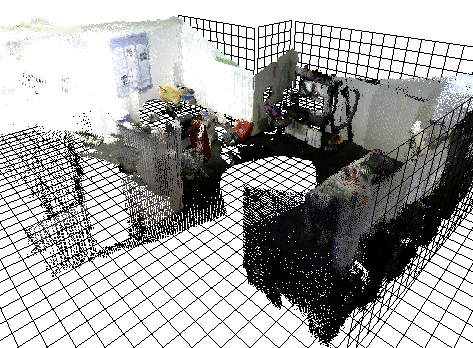
\includegraphics[width=3.0in]{images/ch2/unit21}
                \caption{Apartment}
                \label{fig:RECON_UNIT}
        \end{subfigure}
        \begin{subfigure}[b]{3.0in}
                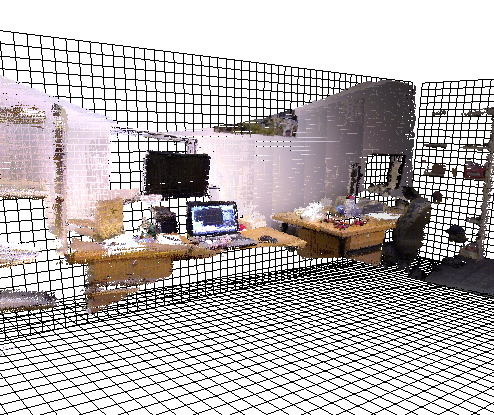
\includegraphics[width=3.0in]{images/ch2/officeA}
                \caption{Office}
                \label{fig:RECON_OFFICE}
        \end{subfigure}
        \begin{subfigure}[b]{3.0in}
                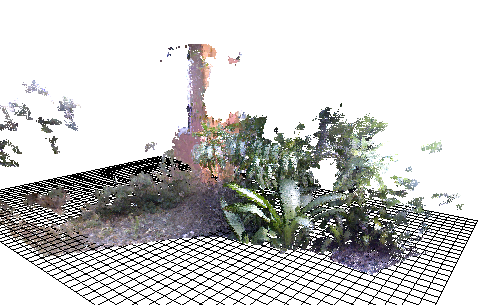
\includegraphics[width=3.0in]{images/ch2/outdoorA}
                \caption{Garden}
                \label{fig:RECON_GARDEN}
        \end{subfigure}
       \caption{Reconstructed Scenes.}
       \label{fig:RECONSTRUCTIONS}
\end{figure}

Qualitative experiments also show the ability of the FVR registration method to reconstruct 3D scenes. In these experiments, two indoor environments (Apartment and Office) as well as one outdoor environment (Garden) were reconstructed and are shown in figures \ref{fig:RECON_UNIT}, \ref{fig:RECON_OFFICE} and \ref{fig:RECON_GARDEN} respectively. \\

The Apartment reconstruction was recorded by moving the ASUS Xtion PRO LIVE active camera through a room and rotating the camera. Each frame was registered using the FVR algorithm. Some of the frames in the apartment scene contain walls which have few features. Between frames, walls also had colour contrast shifts. These shifts are due to the ASUS camera's automatic contrast feature which adjusts contrast based on colour histograms. Despite these setbacks, accurate 3D reconstruction was achieved by the FVR method as illustrated in figure \ref{fig:RECON_UNIT}. \\


The office reconstruction was also generated by rotating the ASUS Xtion PRO LIVE active camera about the y-axis while moving the camera around the room. This time, during rotation, the camera was focused on both foreground and background objects. Here, the entire video sequence was accurately registered. It can be seen that despite the foreground and background focus, the global reconstruction is accurate. This scene, as in the apartment scene has usable texture which should not cause large amounts of texture confusion. These qualitative experiments show that despite being a closed form solution, the FVR has reconstruction accuracy comparable to existing feature based SLAM methods. \\


Typical feature based methods work well with indoor environments where local features are readily distinguishable and easy to match. They do not tend to work as well in complex outdoor scenes where feature confusion is likely. To assess performance in such outdoor scenes, a garden scene containing bushes, plants and a ground covering of bark and rocks was captured for testing. Again, this scene was captured using the ASUS Xtion PRO LIVE active camera moving around the out-door garden. The proposed FVR method was able to produce a good quality reconstruction of this garden scene, as shown in figure \ref{fig:RECON_GARDEN}. This shows that reconstruction approaches which integrate or make use of the FVR registration method may have an advantage in performing 3D reconstructions in these types of scenes, scenes which are of common disturbance to many existing feature matching methods, as expressed in the literature.   



\subsection{Comparison}


Here we present a summary table (Table \ref{tab:GridRT}) to assess the various abilities of each 3D reconstruction algorithm in terms of translation, rotation, scale, non-static object motion robustness and ability to handle various sensory types. In terms of translation, each of the presented algorithms can register with respect to translation. In experiments, it was shown that the FVR algorithm outperforms others when this type of camera movement is present, especially at wider baselines of 10 to 15 cm. In registering rotation, the FVR and FFVR methods are only capable of a single axis of rotation. FVR-3D, however, can register against all 3 axes of rotation. Results have shown that in the presence of rotation, the FVR-3D performs at or above the level of the more accurate algorithms from the literature, ICP and FM2D. It was found that MVVR was not able to handle rotation well, due to the high levels of noise found in the depth maps produced by monocular based techniques. \\

Only the FVR and FVR-3D methods were capable of registering against scale. From the literature, ICP and PCA are not capable of handling such transformations without some modification. Results have shown that these algorithms are capable of handling non-static object motion well. Results on the Kitti Vision benchmark show that FVR-3D outperforms the state-of-the-art, even on data sets which have non-static moving agents. Results also showed that the FVR was the most accurate in the registration of wide baselines, that is translations above 5 cm and rotations above 5 degrees. The FVR algorithm outperformed the others, including the top methods used in the literature. Of these methods, MVVR was shown to be able to register monocular sensor data against translation when noise levels were low. The closer the depth data computed via monocular methods approaches perfectly accurate depth images, the closer the MVVR algorithm approaches FVR performance. In terms of both stereo and active sensor input, FVR, FFVR and FVR-3D are all capable of handling this type of input data well. \\


\begin{table}[h]
\resizebox{\textwidth}{!}{%
\begin{tabular}{ccccccccc}
\textbf{\textit{Algorithm}} & \textbf{translation} & \textbf{rotation} & \textbf{scale} & \textbf{object motion} & \textbf{wide baselines} & \textbf{monocular} & \textbf{stereo} & \textbf{RGB-D}\\ \hline
FVR & yes & 1 axis only & yes & yes & yes & no & yes & yes\\
FFVR & yes & 1 axis only & no & yes & no & no & yes & yes\\
FVR-3D & yes & yes & yes & yes & no & no & yes & yes\\
MMVR & yes & no & no & no & no & yes & no & no\\
\end{tabular}}
\caption{FVR Comparison Table \label{tab:GridRT}}
\end{table}


In summary, the stereo camera and active camera results, show that FVR-3D method outperforms all the other algorithms from the literature. For most of these data sets the FVR algorithm was a strong second place contender. When registering wider baselines, the FVR algorithm was the top performer while FVR-3D fell behind.

%PTPTPT
\section{Plane-Tree Experiments}

In this section, we present experiments in which the Plane-Tree 3D model and 3D reconstruction data compression system are examined. The Plane-Tree is first compared to its similar neighbour method, the octree. It is compared with the octree using the mean error metric discussed in section \ref{metricsSection}. The two algorithms are compared when compressing three commonly available object models, Bunny, Fandisk and Horse. These data are shown in Figure \ref{fig:MODELSUSEDA}. \\

\begin{figure}[!htb]
\centering
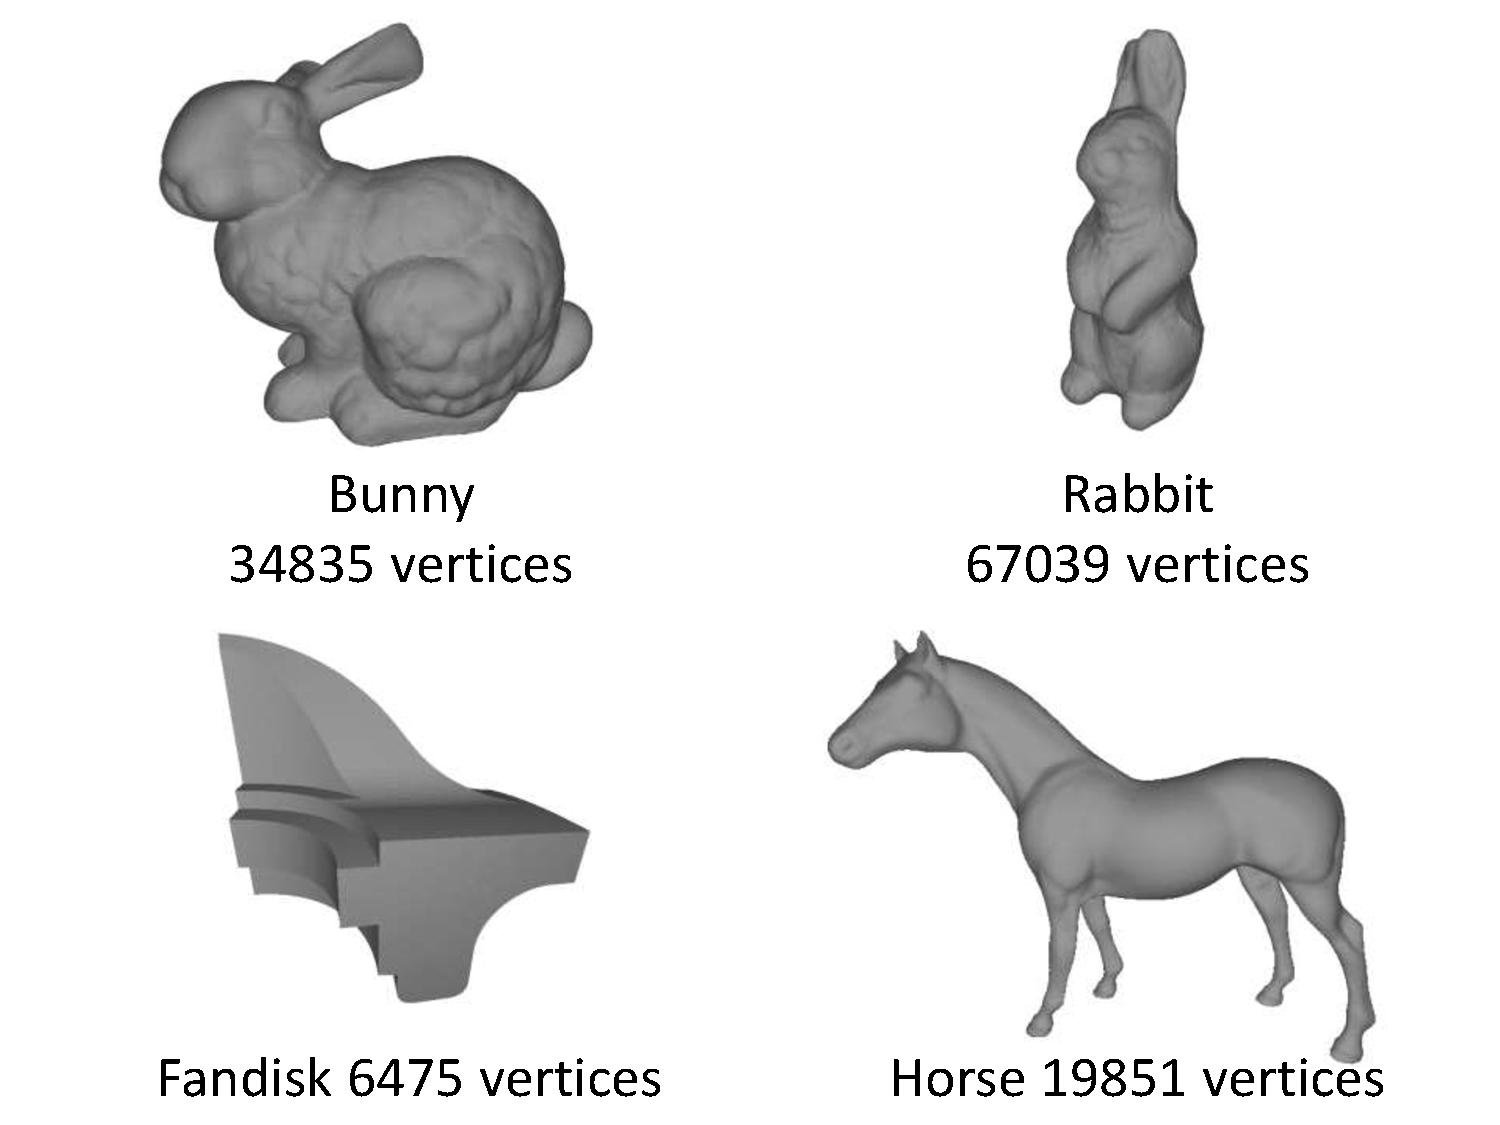
\includegraphics[width=4.0in]{images/experiments/test_data/modelsused}
\caption{Models used to assess the Plane-Tree compression algorithm.}
\label{fig:MODELSUSEDA}
\end{figure}


Next, the Plane-Tree is compared with the current state-of-the-art methods from 3D object compression research. These experiments are presented in section \ref{SEC:PTVSSOTA}. These experiments reveal that the Plane-Tree not only, outperforms the original octree method, but also some of the state-of-the-art transform methods at low-bit-rates. Several state-of-the-art algorithms are compared including some transform based methods \cite{Bayazit103DMesh,Khodakovsky00Progressive} and some compression systems which were designed to compress at low bit-rates \cite{Peng10Feature,Lincoln13Hons}. \\ 

To compare the Plane-Tree with each of these algorithms quantitatively, each algorithm is set-up to compress a model at different levels of compression vs quality. An algorithm's rate-distortion (RD) is plotted and compared to each of the other algorithms. Since lossy algorithms are compared, this indicates the amount of distortion (in the decoded model compared with the original) given a particular bit-rate. This measurement represents the number of bits each algorithm requires to store a particular model at a particular level of quality. The fewer bits required to represent a model of a given accuracy, the better the compression system performs. The mean error and root mean squared error discussed in section \ref{metricsSection} are used to measure the quality of the compressed models whilst the bit-rate in bits per vertex metric is used to measure the number of bits required to store the compressed model. Both the mean error and the root mean squared error are scaled by the main diagonal of the input model to make the results invariant to model size. Qualitative results comparing the Plane-Tree with other state-of-the-art methods are also presented. \\


\section{Plane-Tree vs. Octree}
\label{SEC:PTVSOT}
Figure \ref{fig:OTEXPS} shows rate-distortion graphs comparing the Plane-Tree with the octree compression method. In these rate-distortion graphs we use the mean error between the decoded and input model as the distortion metric. Results show that for the Bunny and Fandisk experiments (Figures \ref{fig:OG_BUNNY} and \ref{fig:OG_FANDISK}) the Plane-Tree has better quality for a given bitrate compared to the octree. It is also evident that the octree is unable to reach the level of quality the Plane-Tree reaches. In both cases, due to the Plane-Tree's ability to prevent further tree decomposition via its more accurate representation method, the Plane-Tree has a much lower error rate for a given bit-rate compared with the octree method. \\

In the Horse model graph in Figure \ref{fig:OG_HORSE} there is some overlap in the model quality (error rates). This overlap ranges from around $0.0025$ to $0.004$ in which for these levels of quality, the octree requires around 8 times more storage space compared with the Plane-Tree. These qualitative results show how much of an improvement the Plane-Tree model codec is over the octree method. \\

\begin{figure}[!htb] 
        \centering
        \begin{subfigure}[b]{2.8in}
                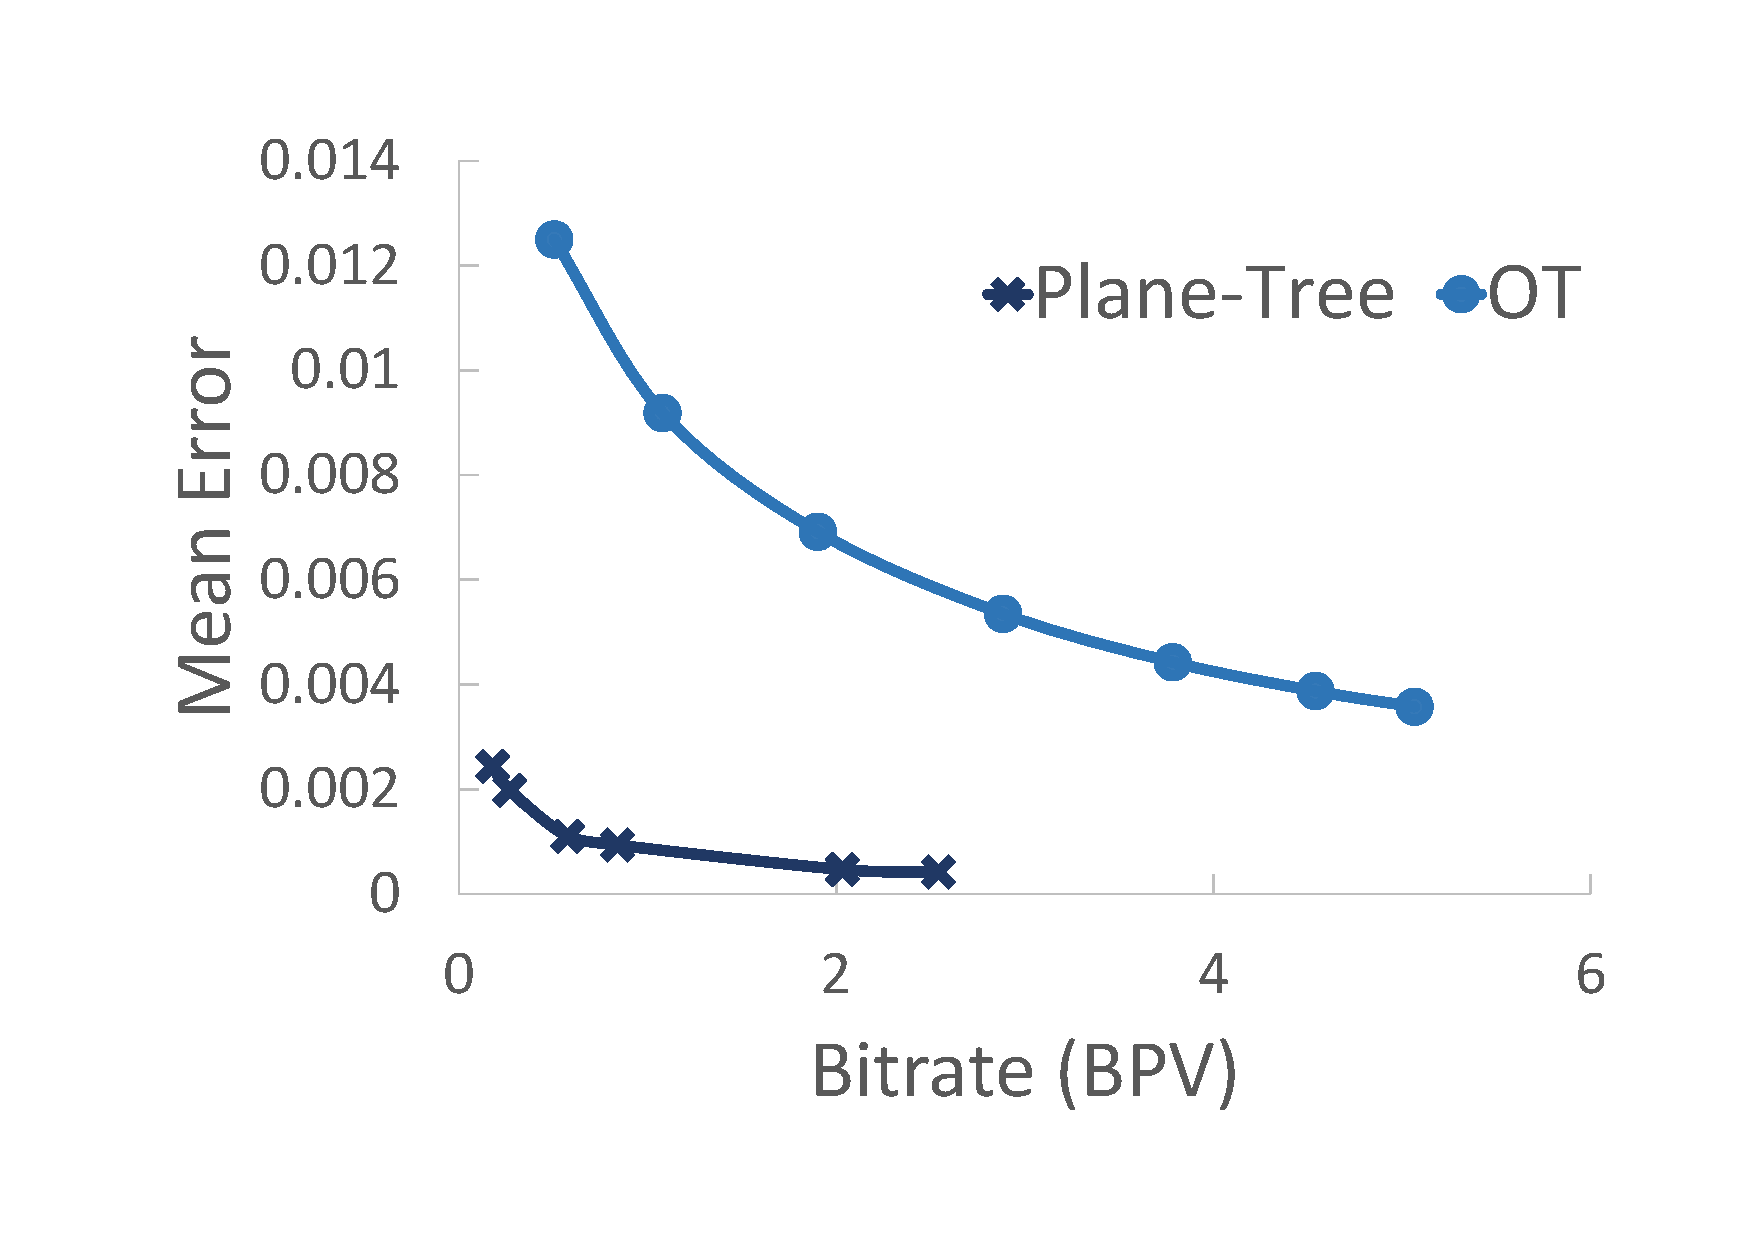
\includegraphics[width=2.5in]{images/results/compression/OTbunny}
                \caption{Bunny Model}
                \label{fig:OG_BUNNY}
        \end{subfigure}%
        \begin{subfigure}[b]{2.8in}
                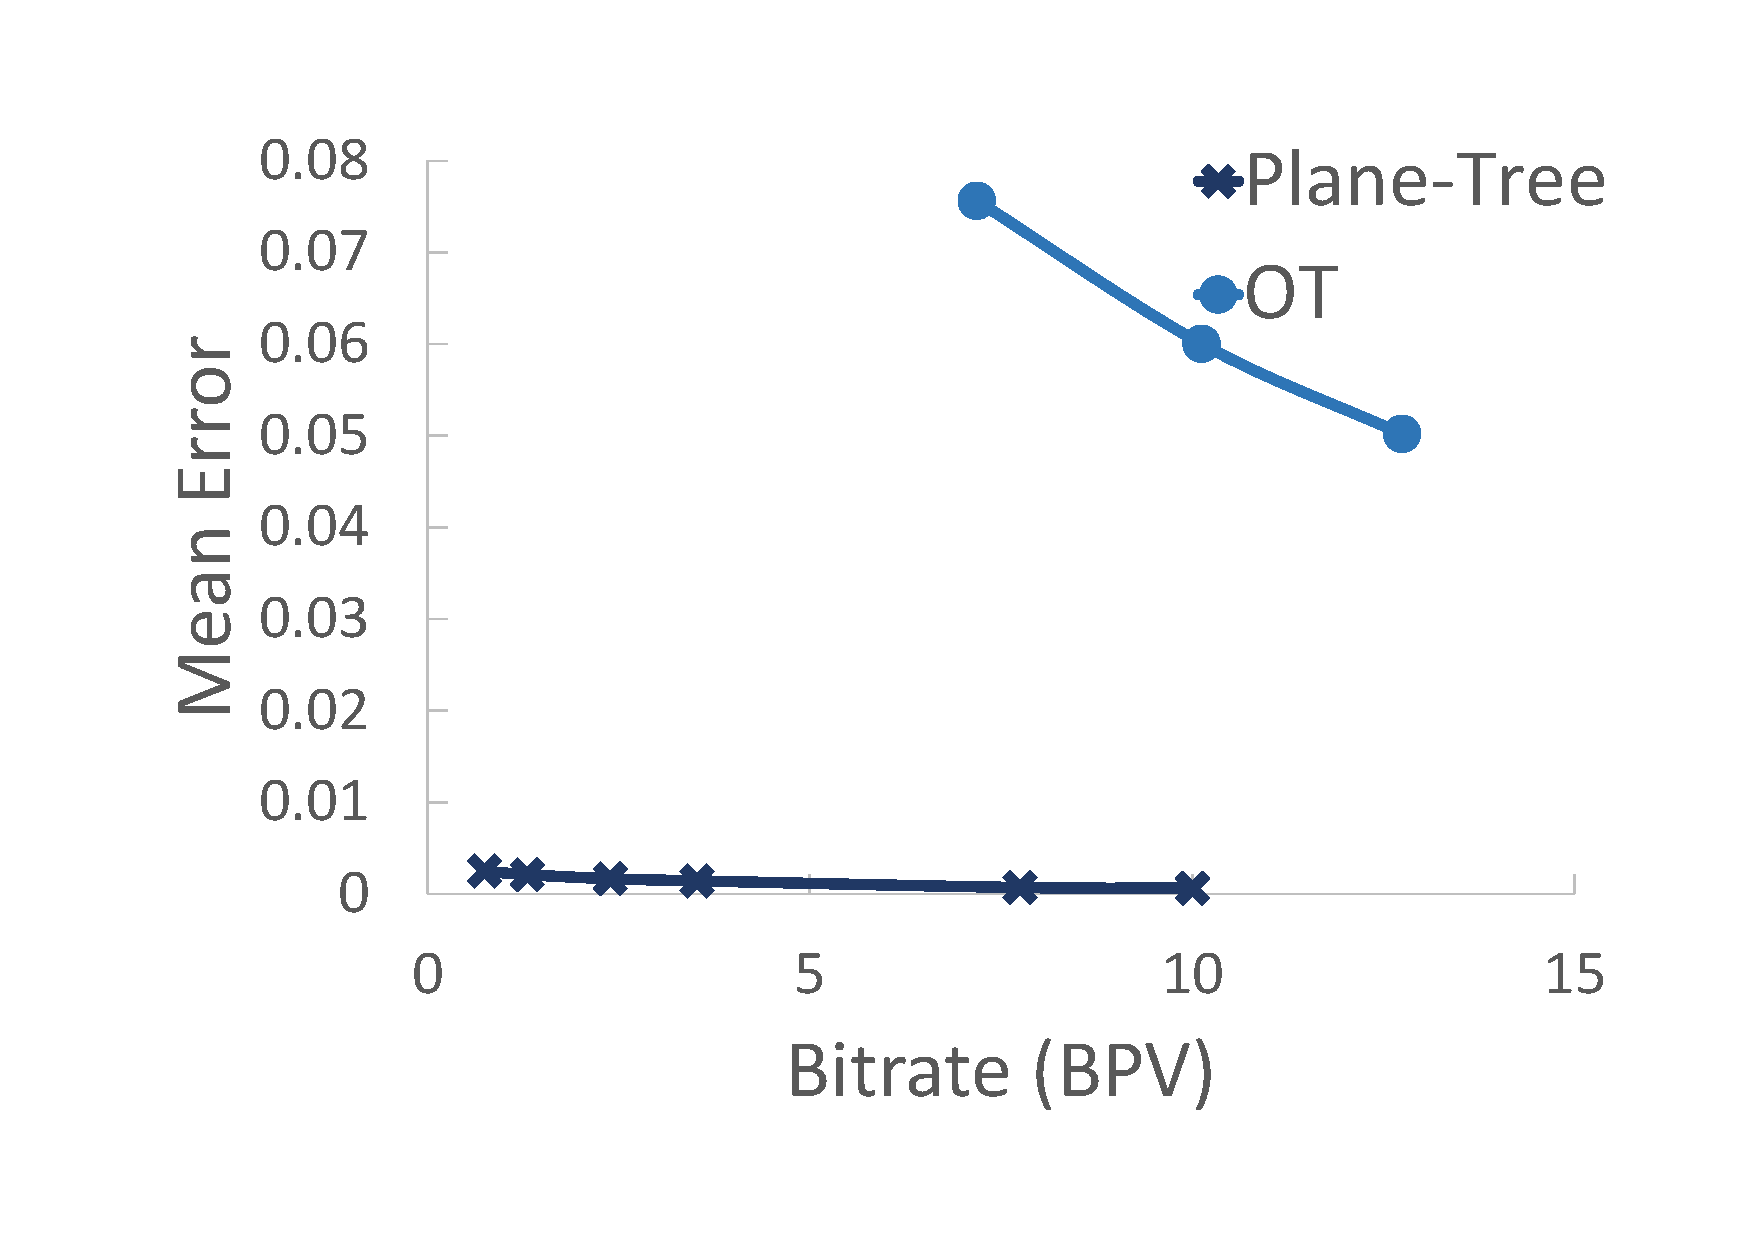
\includegraphics[width=2.5in]{images/results/compression/OTFandisk}
                \caption{Fandisk Model}
                \label{fig:OG_FANDISK}
        \end{subfigure}
        
        \begin{subfigure}[b]{2.8in}
                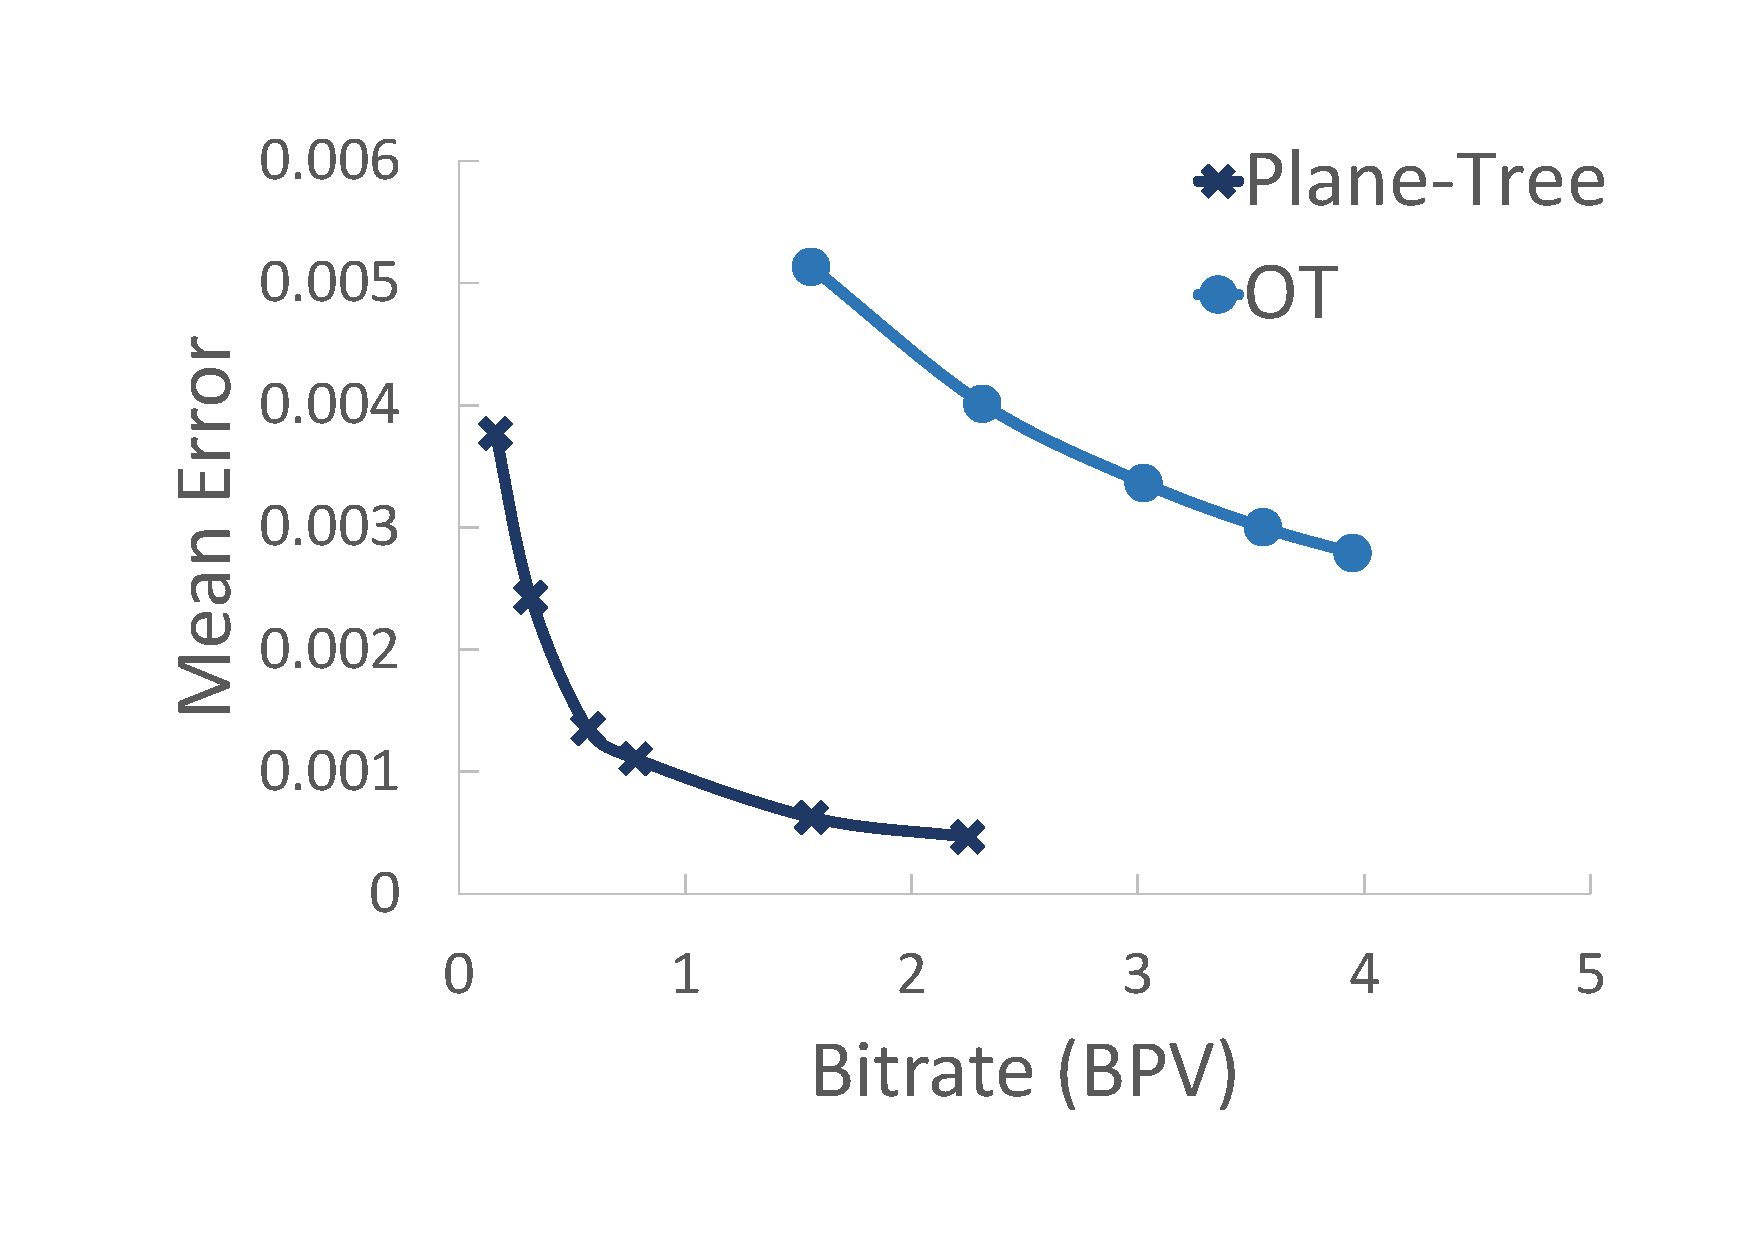
\includegraphics[width=2.5in]{images/results/compression/OTHorse}
                \caption{Horse Model}
                \label{fig:OG_HORSE}
        \end{subfigure}%

       \caption{Rate-distortion graphs comparing the Plane-Tree with the Octree.}
       \label{fig:OTEXPS}
\end{figure}
\section{Plane-Tree vs. Existing Techniques}
\label{SEC:PTVSSOTA}
\subsection{Pose Estimation Results}

These experiments measured registration error for the data sets mentioned in the test data section. As mentioned, different camera movements and scene types are used. Different camera movements such as translation, rotation and zoom were used. The different scenes used include: in-door, out-door, low-textured areas, large object frames areas and areas which include texture confusion. \\


\begin{figure*}[t]
\centering
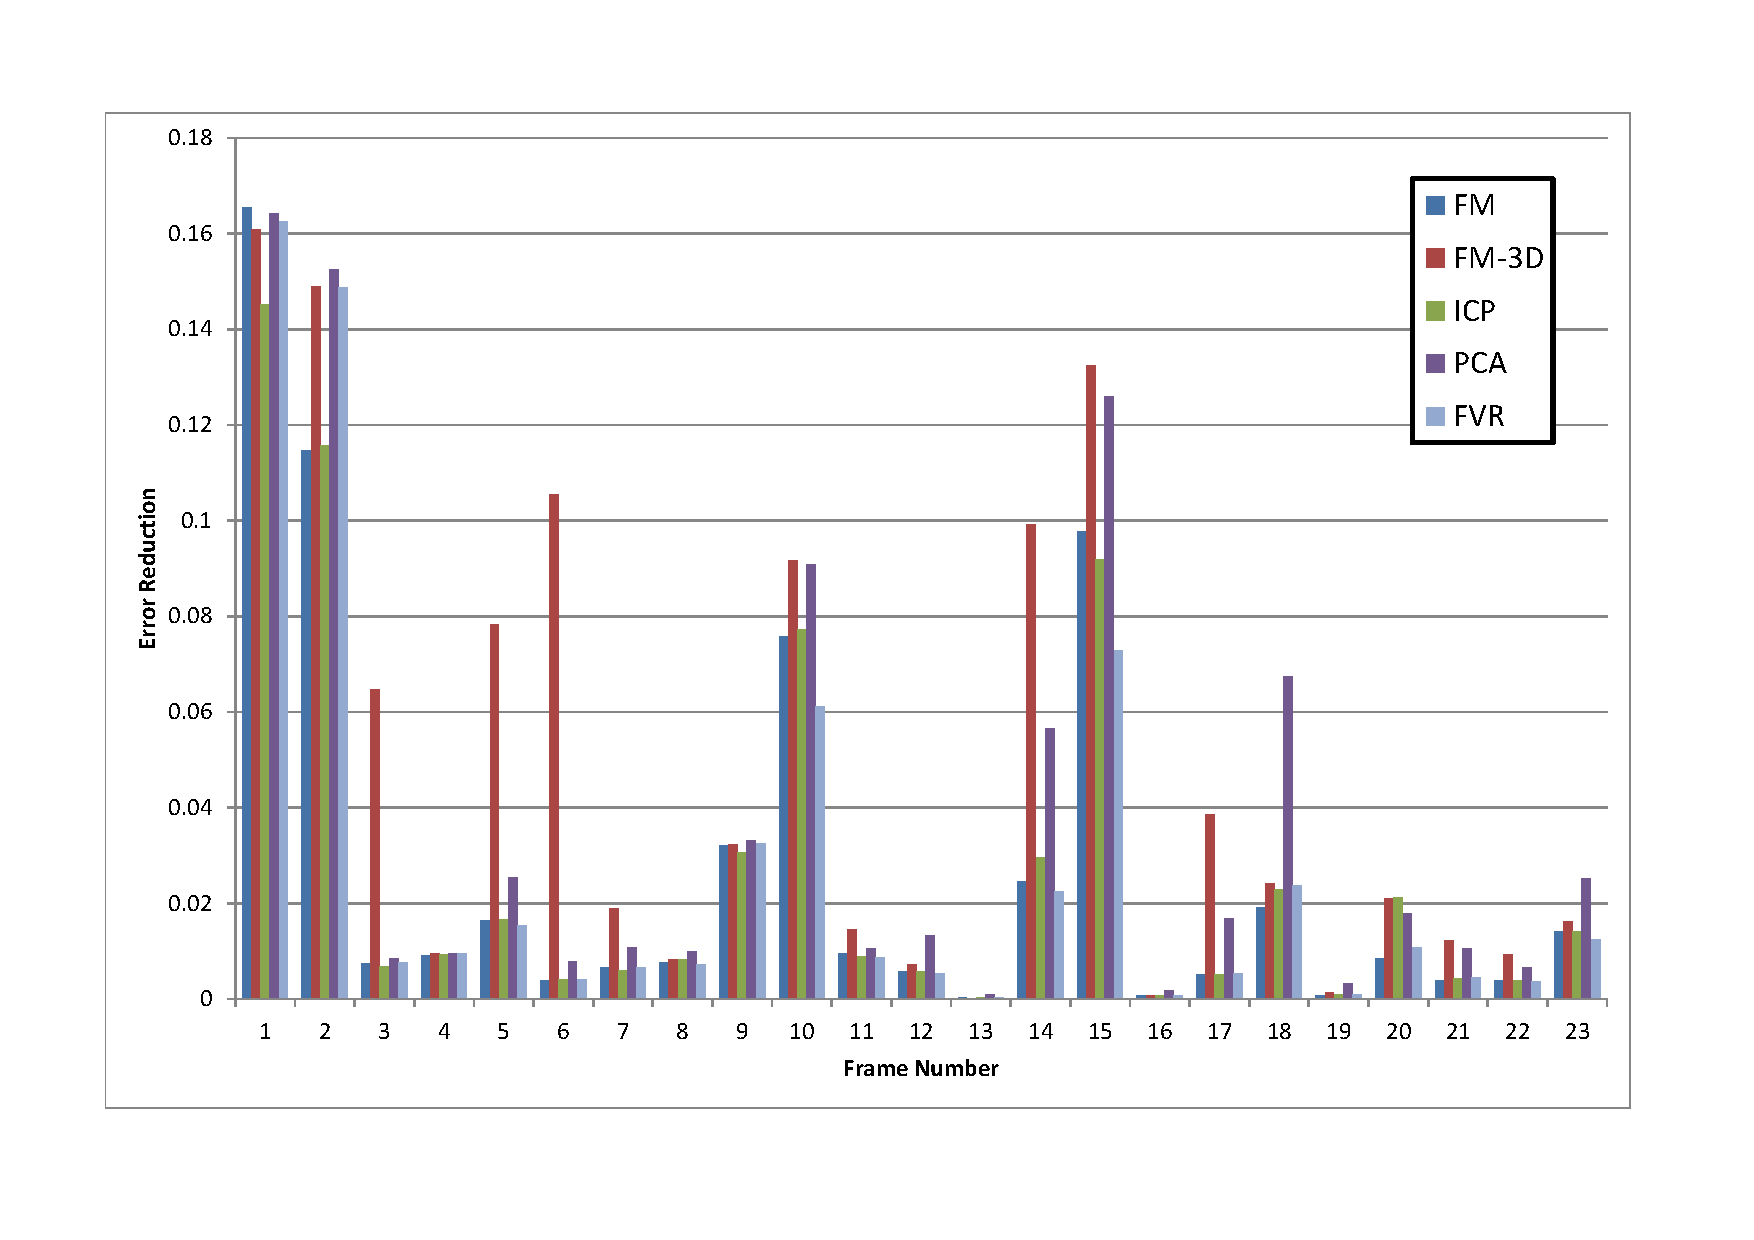
\includegraphics[width=6.0in]{images/results/Apartment_Texture_Rotate}
\caption{Registration Error for the Apartment Y-Axis Rotation Data Set}
\label{fig:PET0}
\end{figure*}

The first experiment was performed with the textured apartment data-set \ref{fig:PET0}. In each of these graphs, the x-axis represents the frame number (in which the previous frame was matched to) and the y-axis represents the registration error in Hausdorff distance relative to performing zero registration. For identical point-clouds, a Hausdorff error above 1 would mean a failure to register in any way, whilst a 0 would mean a complete registration. Since frames do not overlap, it would be improbably to get 0, and a registration error of 1 or above may still be considered good, especially if there was not much overlap in the first place. \\


\begin{figure*}[t]
\centering
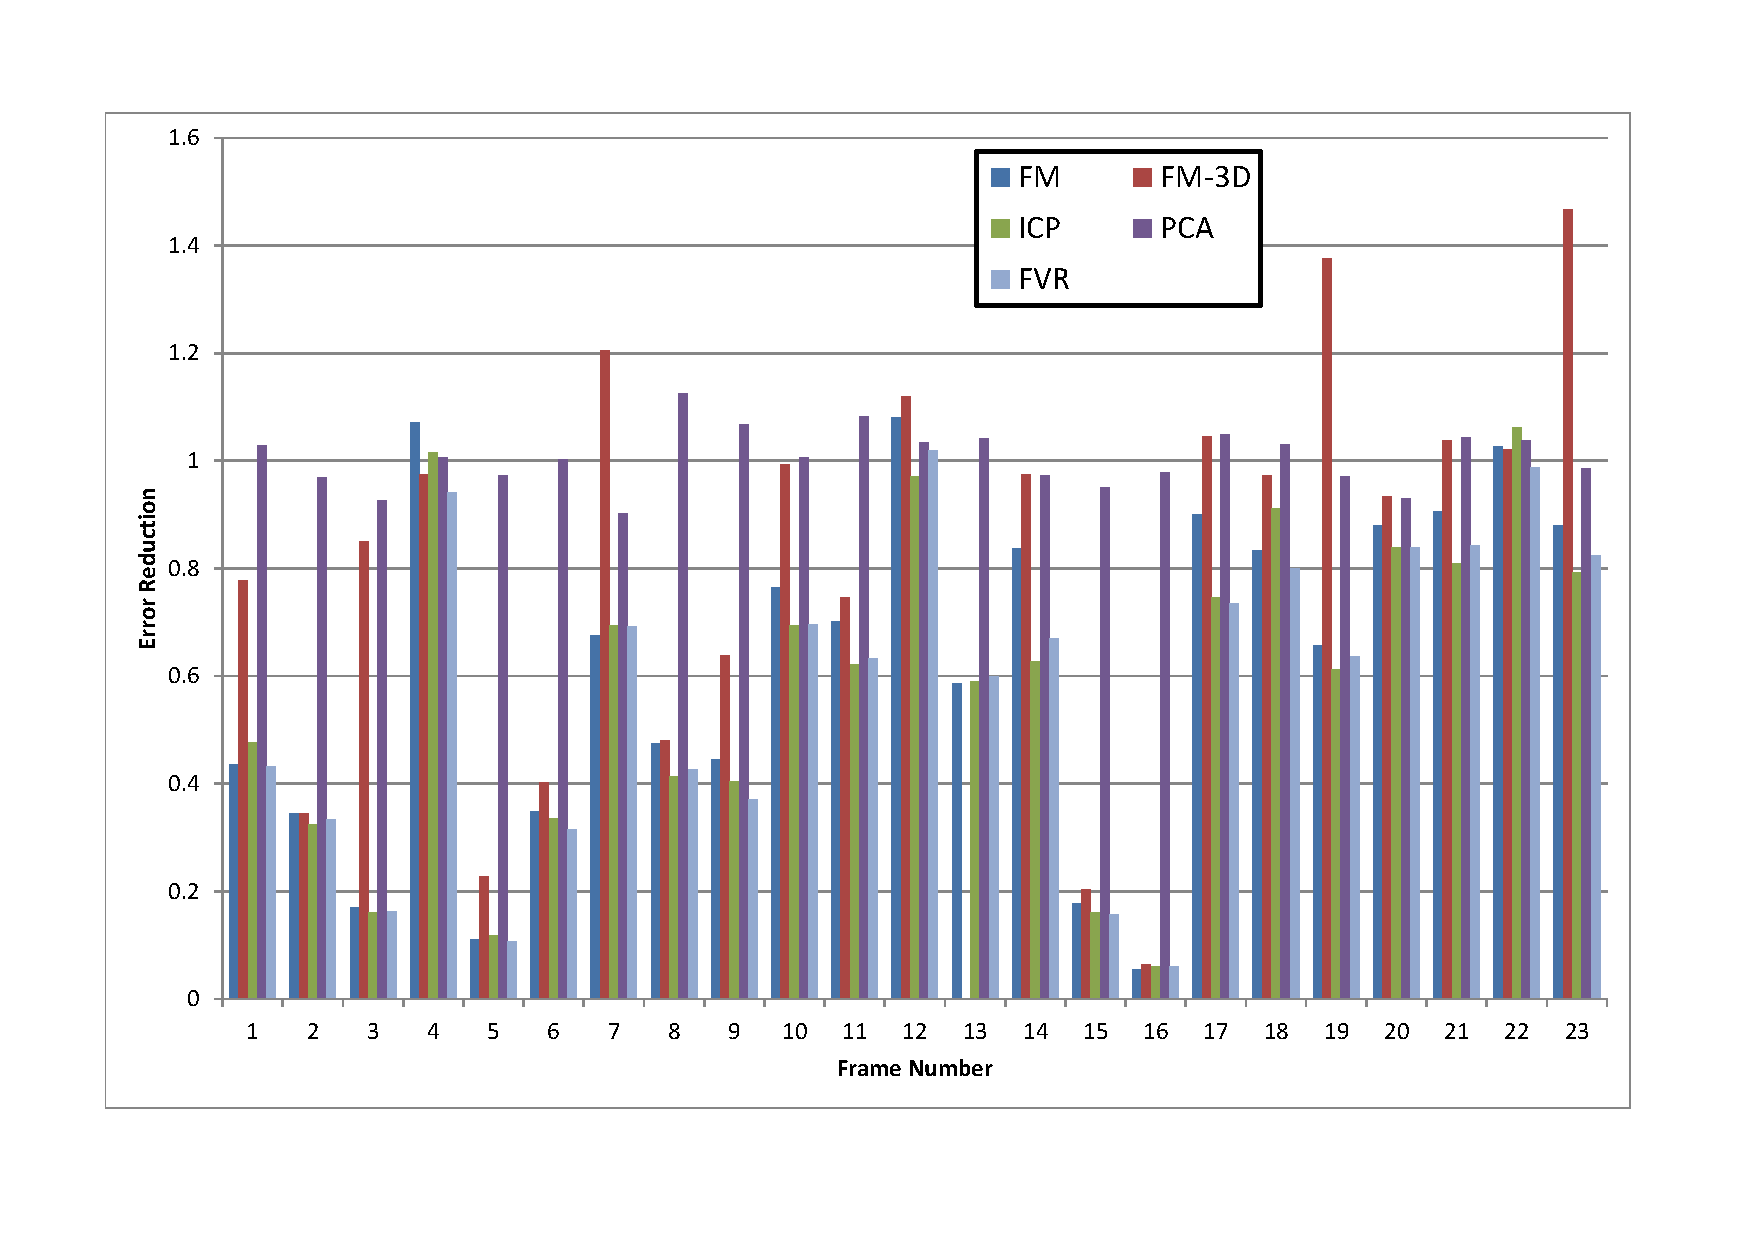
\includegraphics[width=6.0in]{images/results/Apartment_Texture_Rotate_XAxis}
\caption{Registration Error for the Apartment X/Y-Axis Rotation Data Set}
\label{fig:PET1}
\end{figure*}

In figure \ref{fig:PET0}, feature-matching, 3D-feature-matching, ICP, PCA and Fourier Volume Registration (FVR) were tested. In the first frame, FVR only outperformed feature-matching and PCA. In a few of the frames, the 3D feature matching and the PCA methods performed poorly relative to the reset, on other frames they were on par with others. In some frames FVR outperformed the others, this occurred on 13 out of the 23 frames tested (about 60\%). This was not completely expected as for this scene, where much texture is present, feature matching should have dominated. The frames were not highly separated so ICP should have gotten a better result too. Although ICP could be said to be very consistent.

\begin{figure*}[t]
\centering
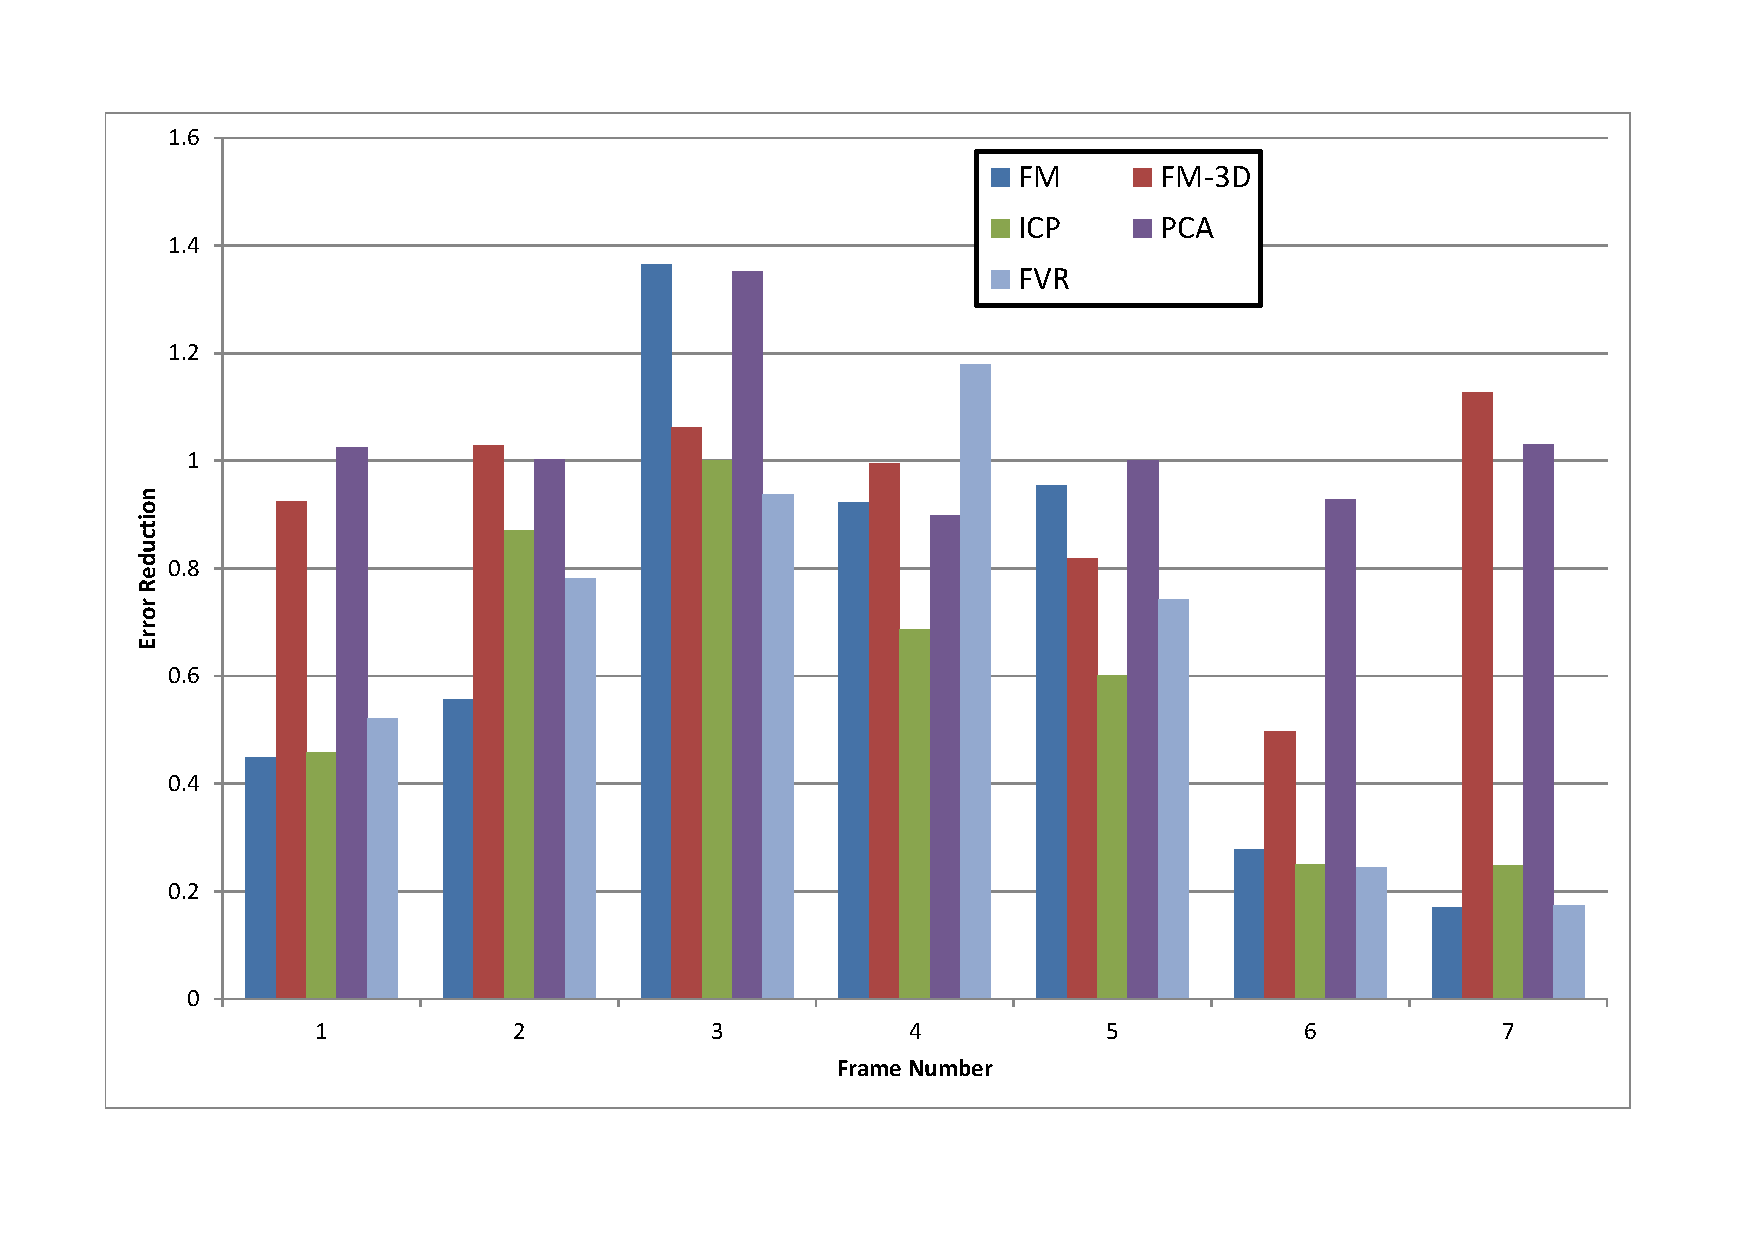
\includegraphics[width=6.0in]{images/results/Boxes_Texture_Rotate}
\caption{Registration Error for the Boxes Y-Axis Rotation Data Set}
\label{fig:PET2}
\end{figure*}

Figure \ref{fig:PET1} shows registration errors for the same scene, the apartment, this time the camera is moved about the x-axis predominantly, again it contains lots of texture. In a about 60\% of the frames, FVR either outperforms or matches the best performing algorithm. Here, ICP and 2D-feature matching are also very competitive, with 3D-feature-matching and PCA failing. In the case of PCA, when there is not enough overlap PCA fails to compute the principal components well. When FVR uses PCA, it only uses the primary axis, and can iteratively refine the alignment in a second stage.

\begin{figure*}[t]
\centering
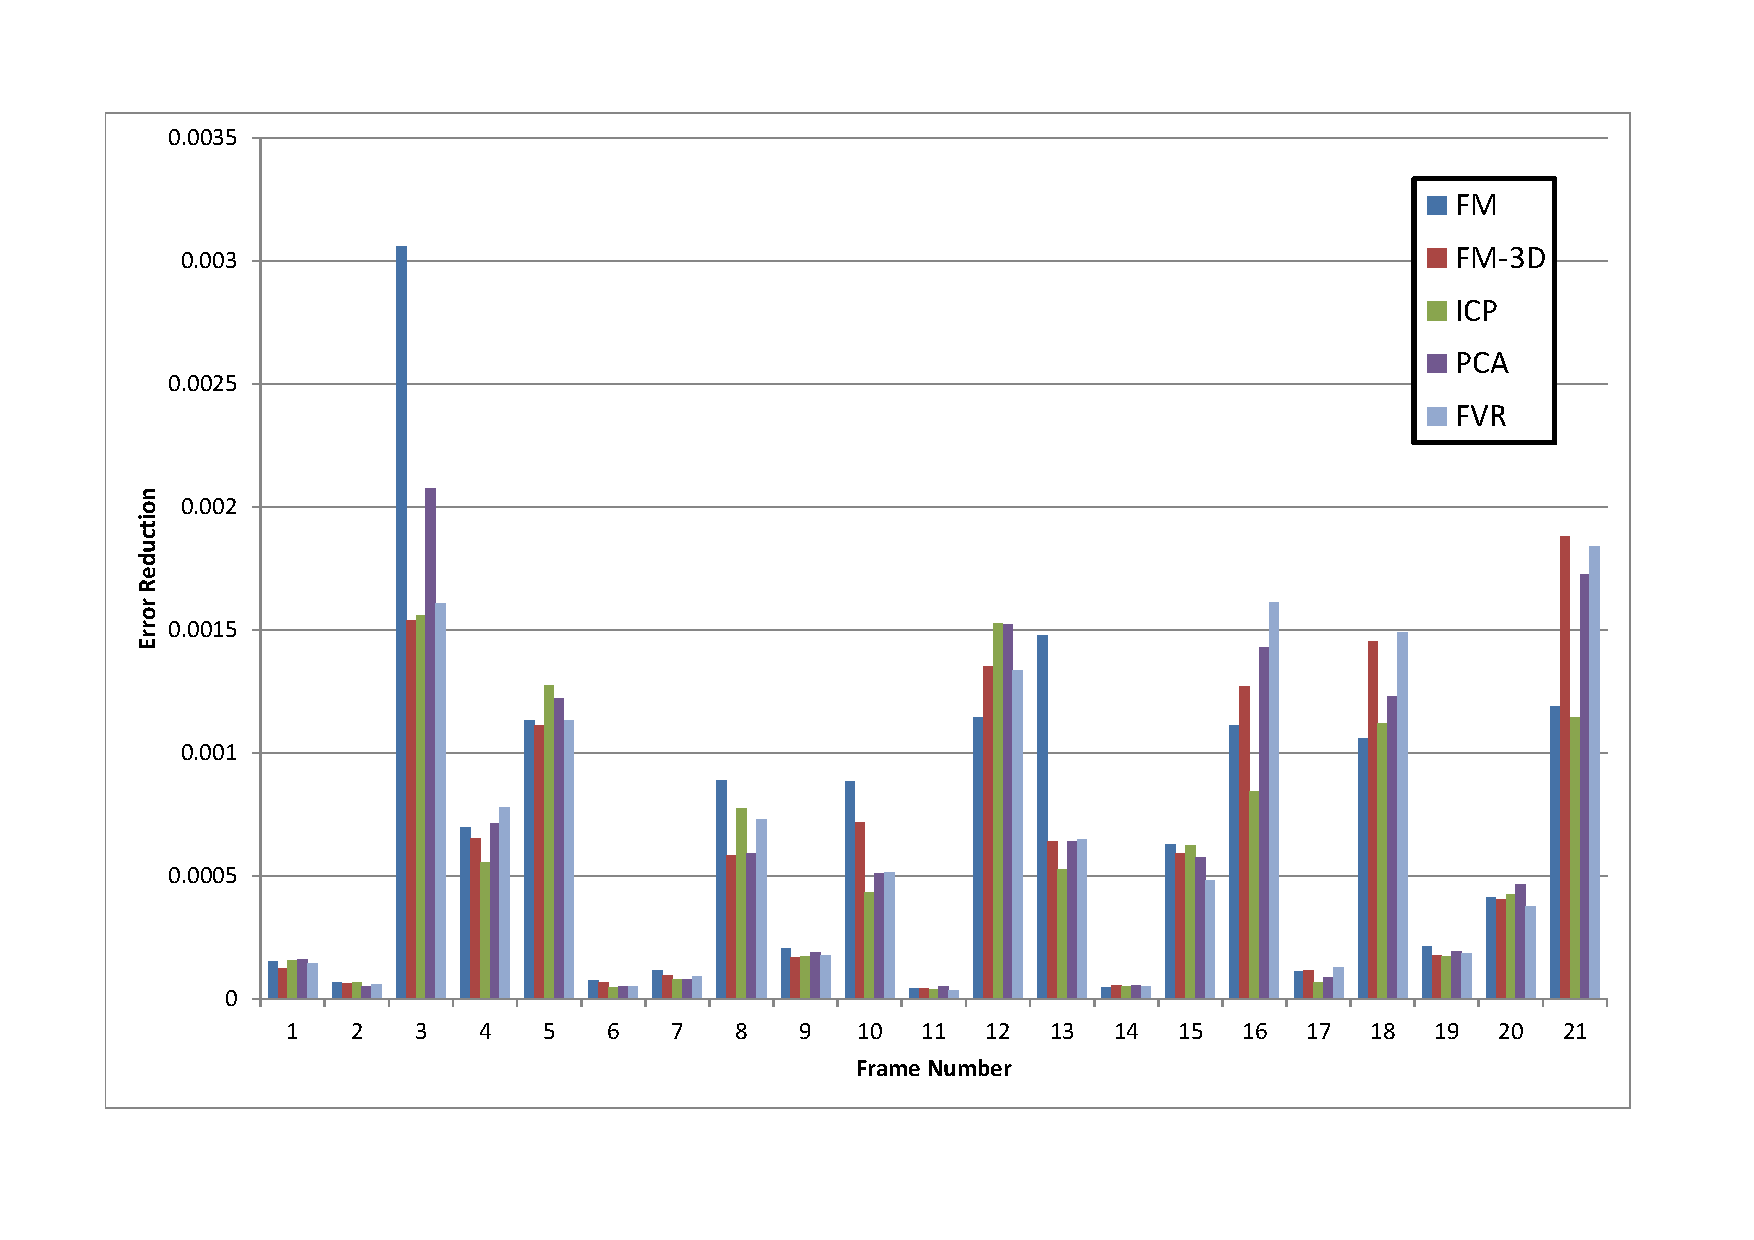
\includegraphics[width=6.0in]{images/results/Boxes_Texture_ZoomOut}
\caption{Registration Error for the Boxes Zoom Data Set}
\label{fig:PET3}
\end{figure*}

In figure \ref{fig:PET2} 7 registration errors are shown in a graph. In 4 out of the 7 frames, FVR outperformed the other algorithms. Note in frame 3, both PCA and feature-matching failed, despite texture being present in the scene. In frames 4 and 5, ICP outperformed the others by a successful margin. 

\begin{figure*}[t]
\centering
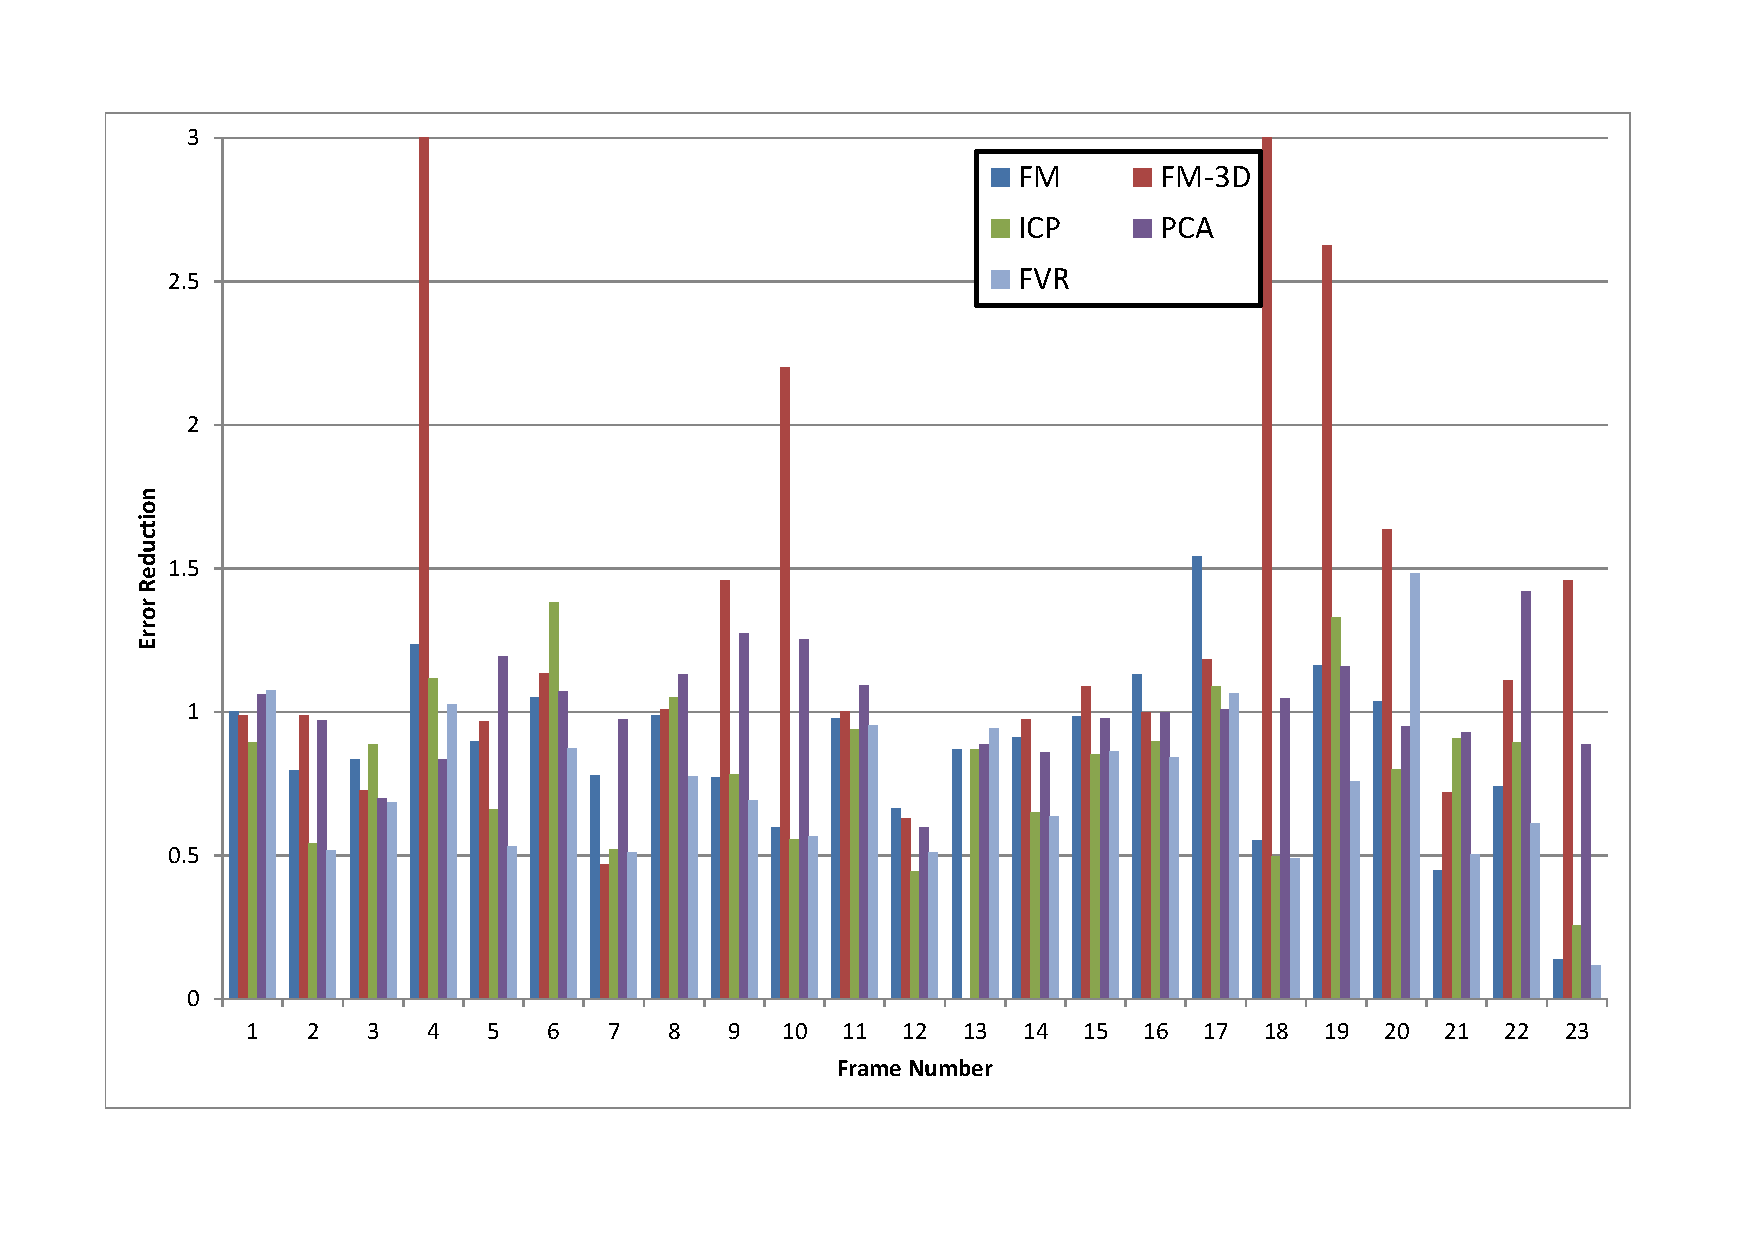
\includegraphics[width=6.0in]{images/results/Desk_Texture_Translation}
\caption{Registration Error for the Desk Translation Data Set}
\label{fig:PET4}
\end{figure*}

Experiment results for the boxes scene where the camera was moved forward, effectively zooming in on the boxes, are shown in figure \ref{fig:PET3}. Here, only 10 out of the 21 (~47\%) of the frames had a registration error lowest or equal for FVR. In a rare case, frame 16 observed a worst performance by FVR. In frame 3, 2D-feature-matching performed the worst, and towards the last few frames PCA and 3D-feature-matching performed worst.

\begin{figure*}[t]
\centering
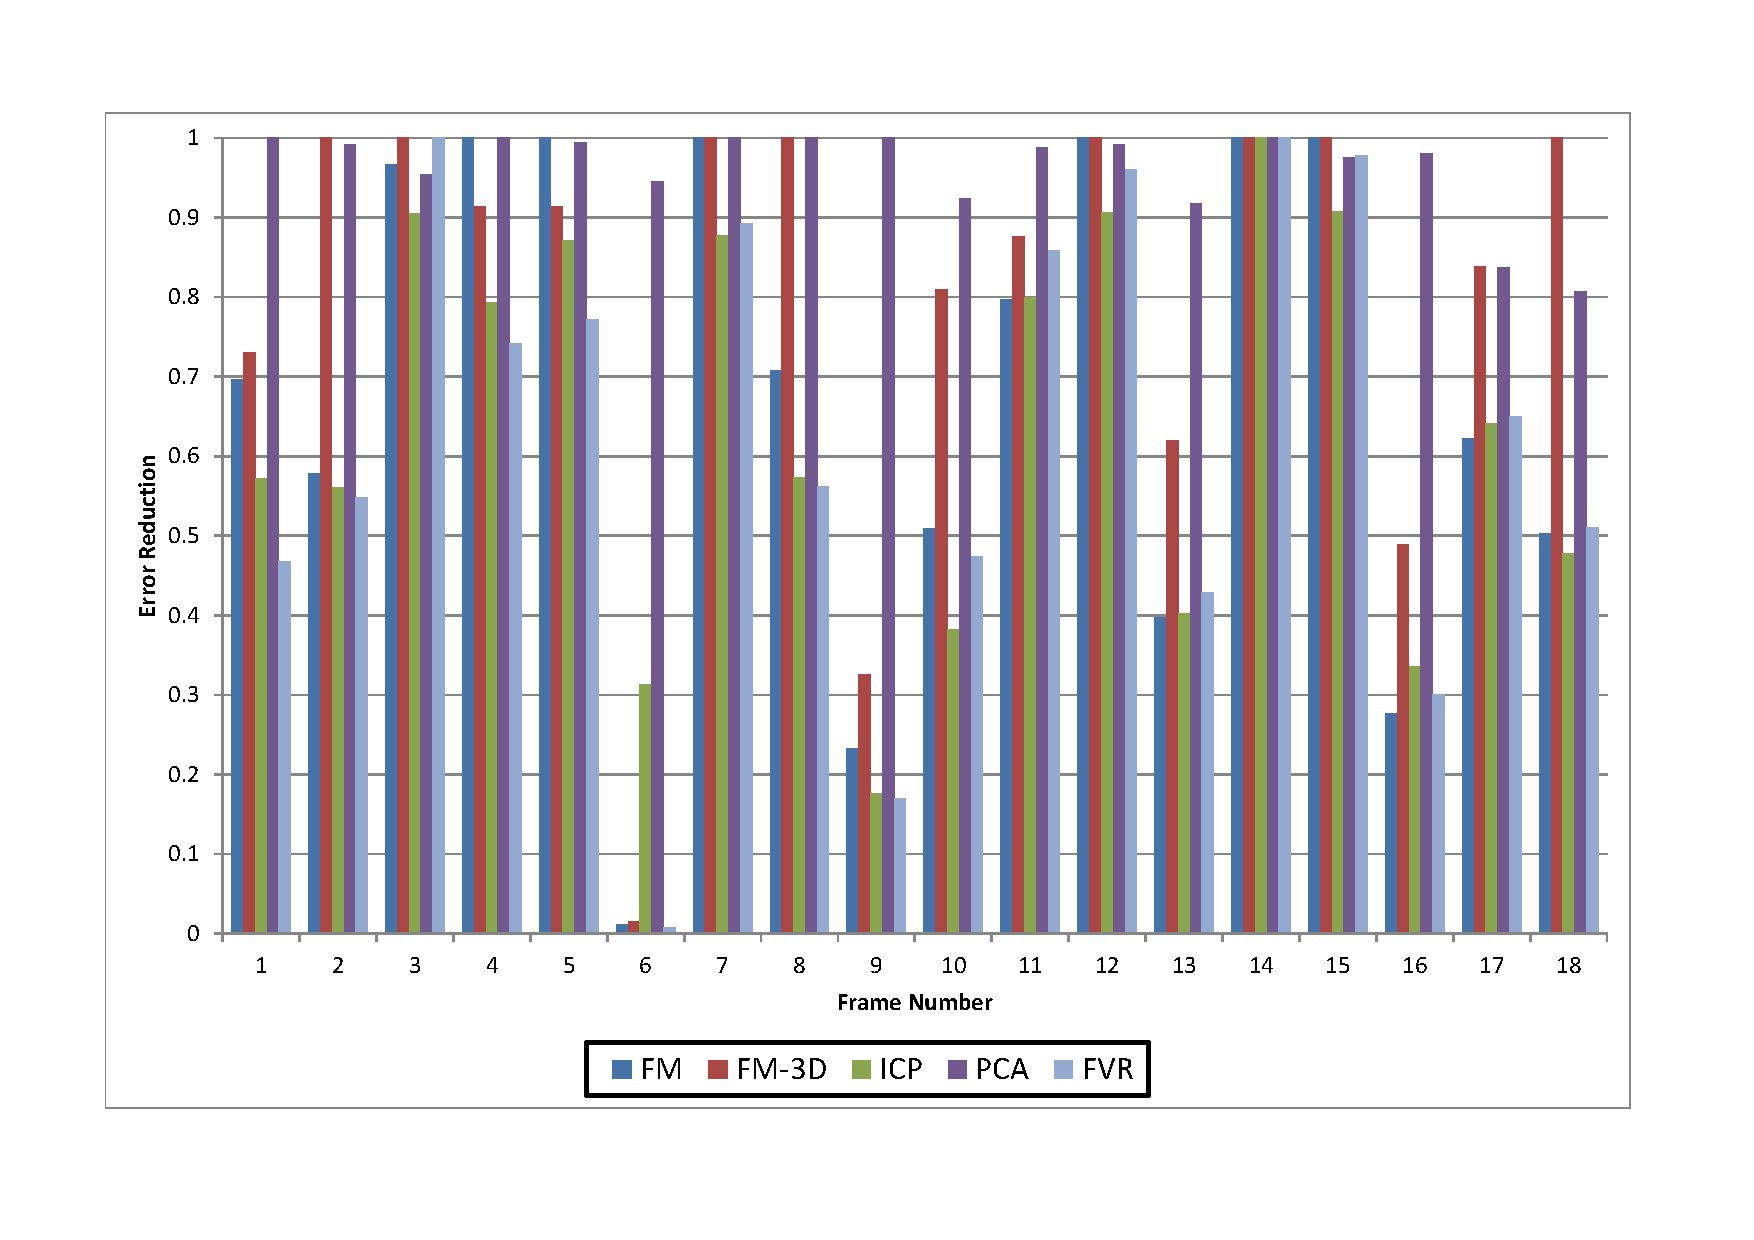
\includegraphics[width=6.0in]{images/results/IndoorSpace_texture_confusion_translation}
\caption{Registration Error for the Texture Confusion Indoor-Space Translation Data Set}
\label{fig:PET5}
\end{figure*}

In ~52\% of the frames of the desk translation data-set in figure \ref{fig:PET4}, the FVR method outperformed others relative to just ~26\% for ICP, ~9\% for 2D-feature-matching and PCA and ~4\% for 3D-feature-matching. This data-set tested for the pose-estimation procedure's ability to align a moving camera along a path. 3D feature matching was a notable poor performer here, ICP and FVR seemed to be strongest. 


\begin{figure*}[t]
\centering
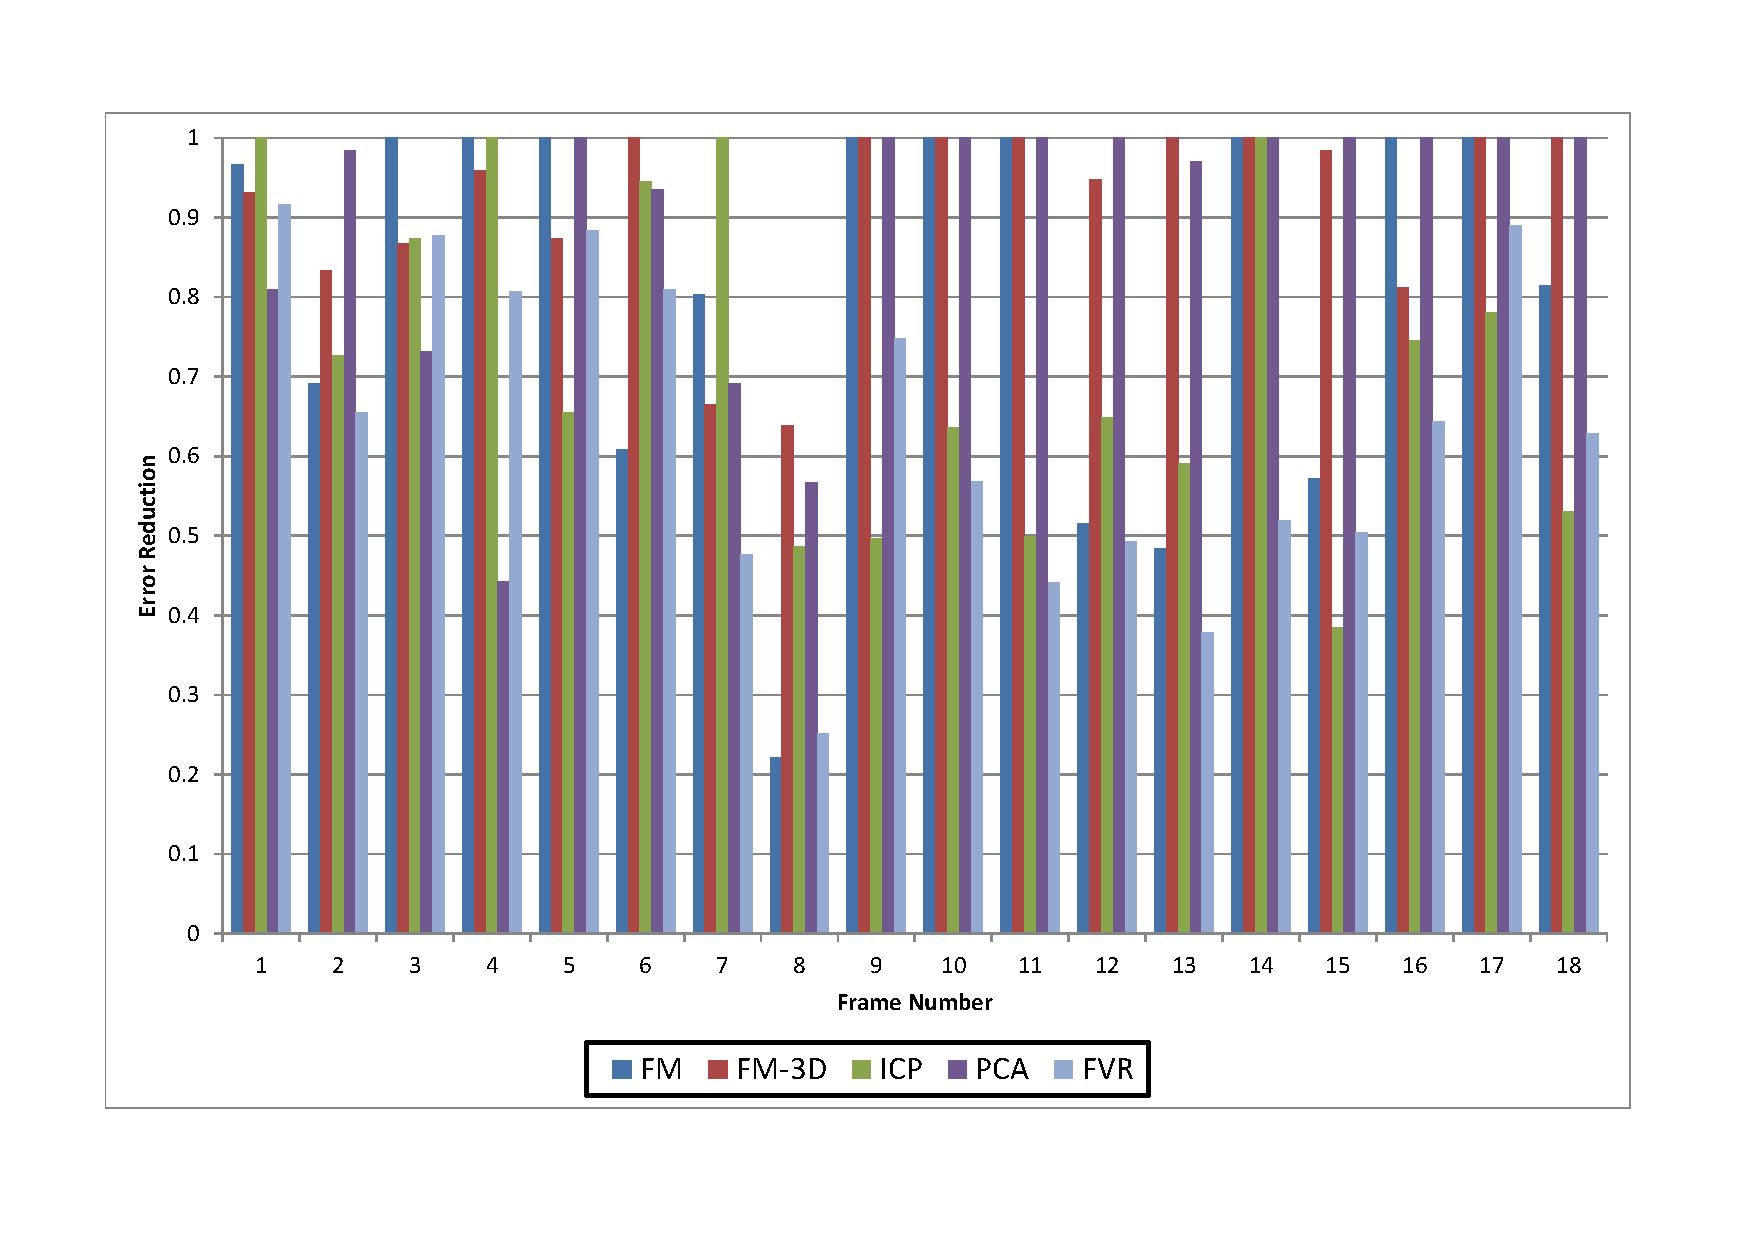
\includegraphics[width=6.0in]{images/results/Kitchen_LittleTexture_Pan}
\caption{Registration Error for the Low-Texture Kitchen Translation Data Set}
\label{fig:PET6}
\end{figure*}

An important data-set tested is the Indoor-Space with texture confusion (figure \ref{fig:PET5}). Here, a small scene was observed, where texture-confusion was present, this makes registration more difficult for all algorithms most notably the feature matching methods. We suspected that ICP, PCA, and FVR would perform best here. Here, around 39\% of the time, FVR performed best. Compared to the best feature-matching method (2D) with ~22\% of performances being the best. Interestingly PCA performed much worse compared with 2D-feature-matching. ICP outperformed others around 33\% of the time, similar to FVR's position but not quite as good. 

Results for the low-textured Kitchen data-set were collected and shown in figure \ref{fig:PET6}. Again around 44\% of the frames had best results given by FVR. Compared with the next best algorithm ICP at ~27\%. In this case, this is expected as the feature-matching methods should perform worse in a low-textured scene. PCA was next best having the best registration ~22\% of the time.

\begin{figure*}[t]
\centering
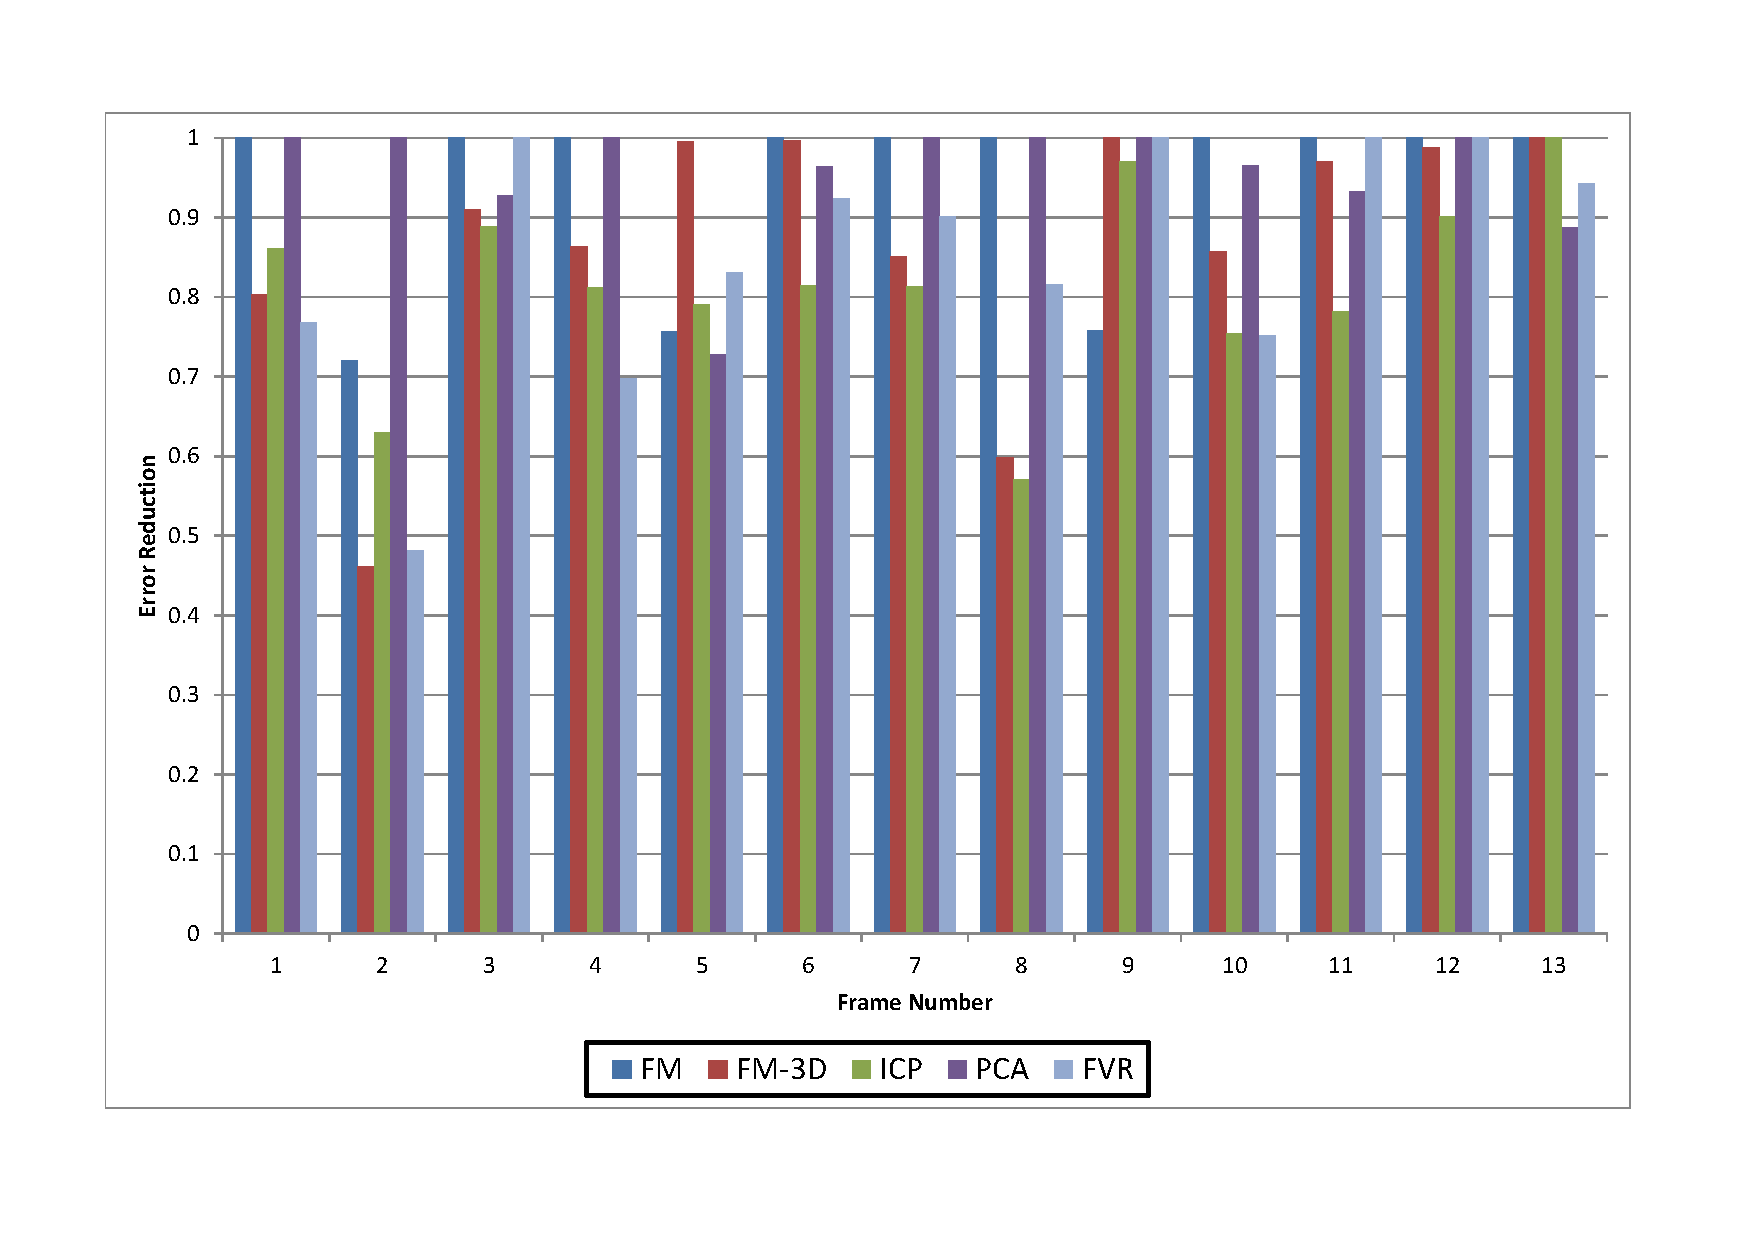
\includegraphics[width=6.0in]{images/results/Kitchen_Little_Texture_Zoom}
\caption{Registration Error for the Low-Texture Kitchen Zoom Data Set}
\label{fig:PET7}
\end{figure*}

Another test for the low-textured Kitchen scene was also performed, this time by moving the camera forward and backwards, zooming in on the scene. In this test, FVR only outperformed the other methods in 3 out of the 13 frames. ICP outperformed FVR on this data-set, as 6 out of the 5 frames had best results given by ICP. It could also be said that ICP was a little more consistent. Interestingly 3D-feature-matching outperformed the 2D counterpart.

\begin{figure*}[t]
\centering
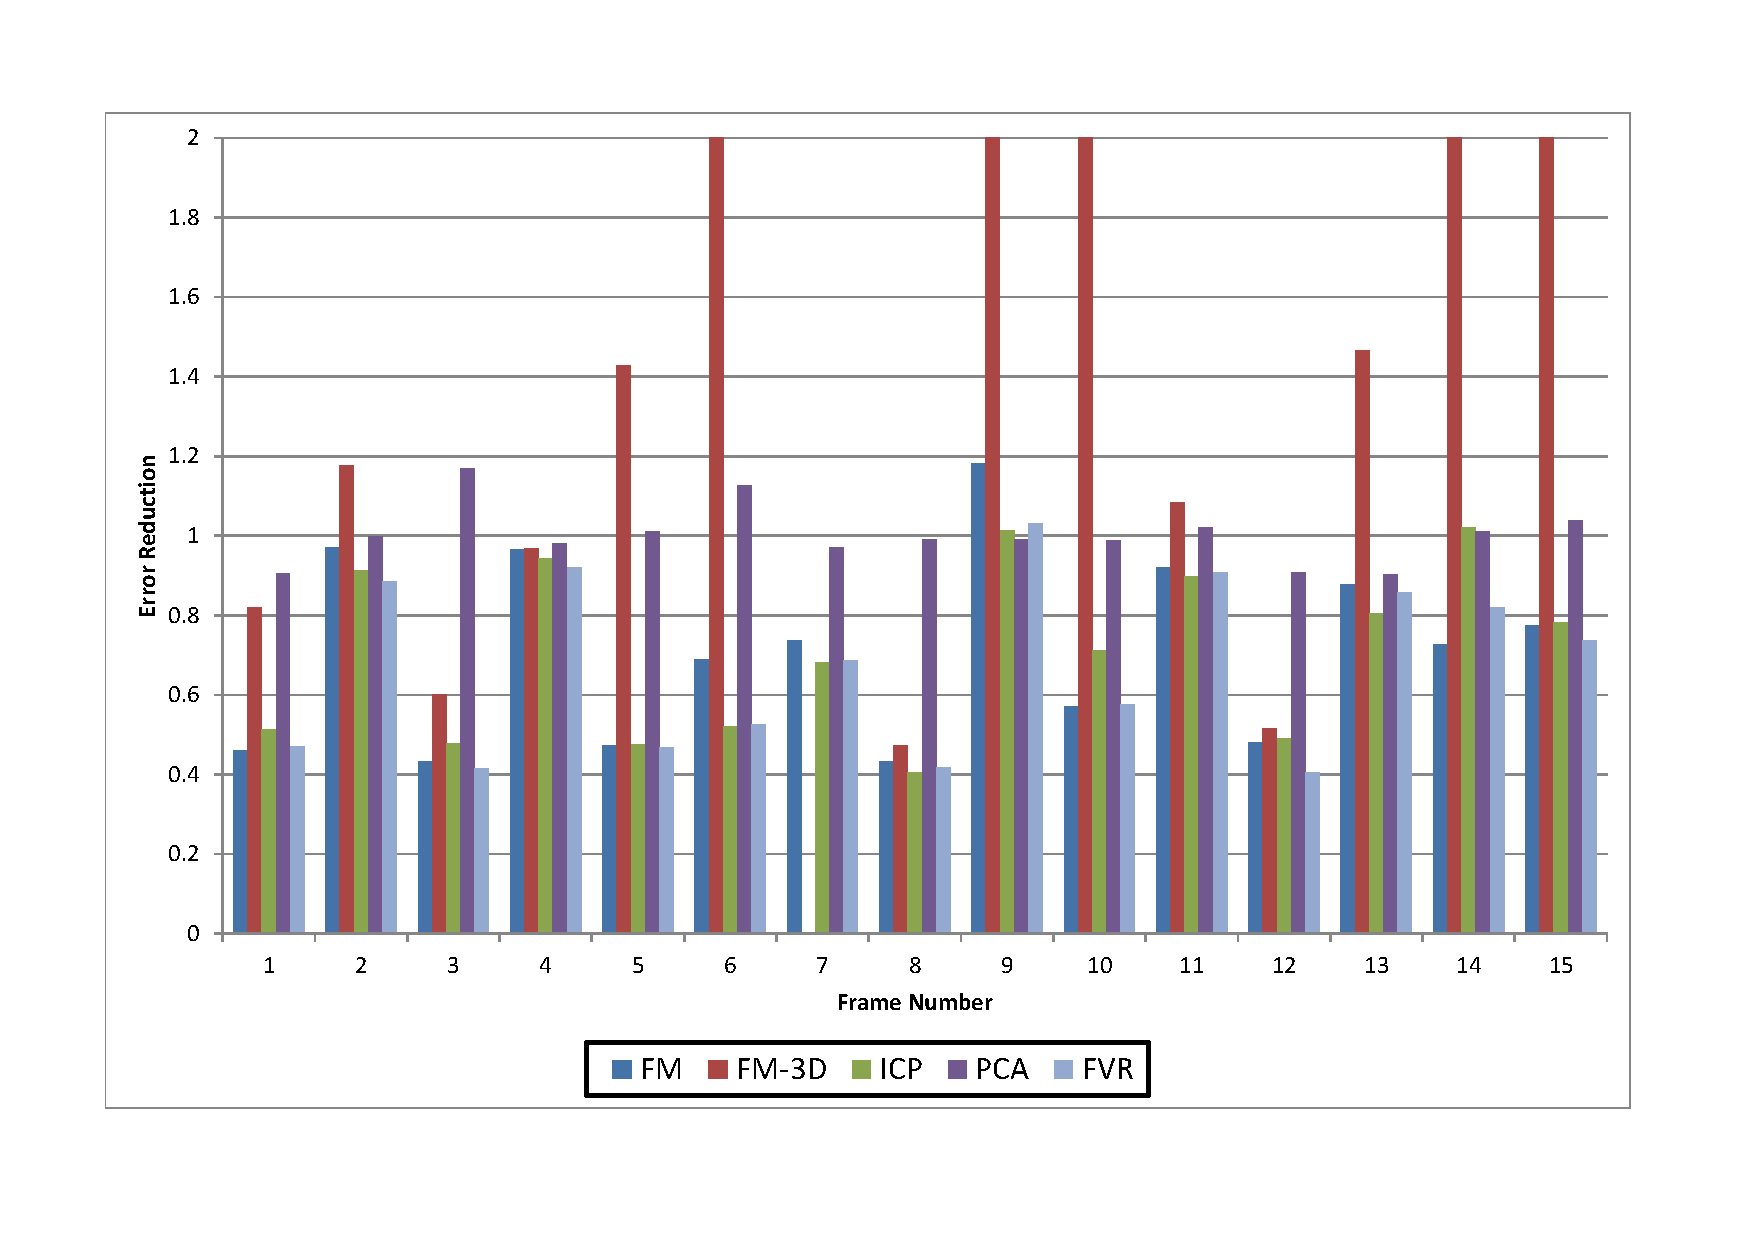
\includegraphics[width=6.0in]{images/results/Office_TexturedItems_Translation}
\caption{Registration Error for the Office Translation Data Set}
\label{fig:PET8}
\end{figure*}

In the results for the Textured Office set (figure \ref{fig:PET8}), FVR matched or beat the other algorithms 80\% of the time. 2D-feature matching also performed well but did not manage to best FVR most of the time. This results shows that, to our surprise, FVR not only works well compared to other algorithms in scenes with little or no texture or in scenes where feature confusion is high, but also in high texture scenes where feature-matching should have an advantage.


\begin{figure*}[t]
\centering
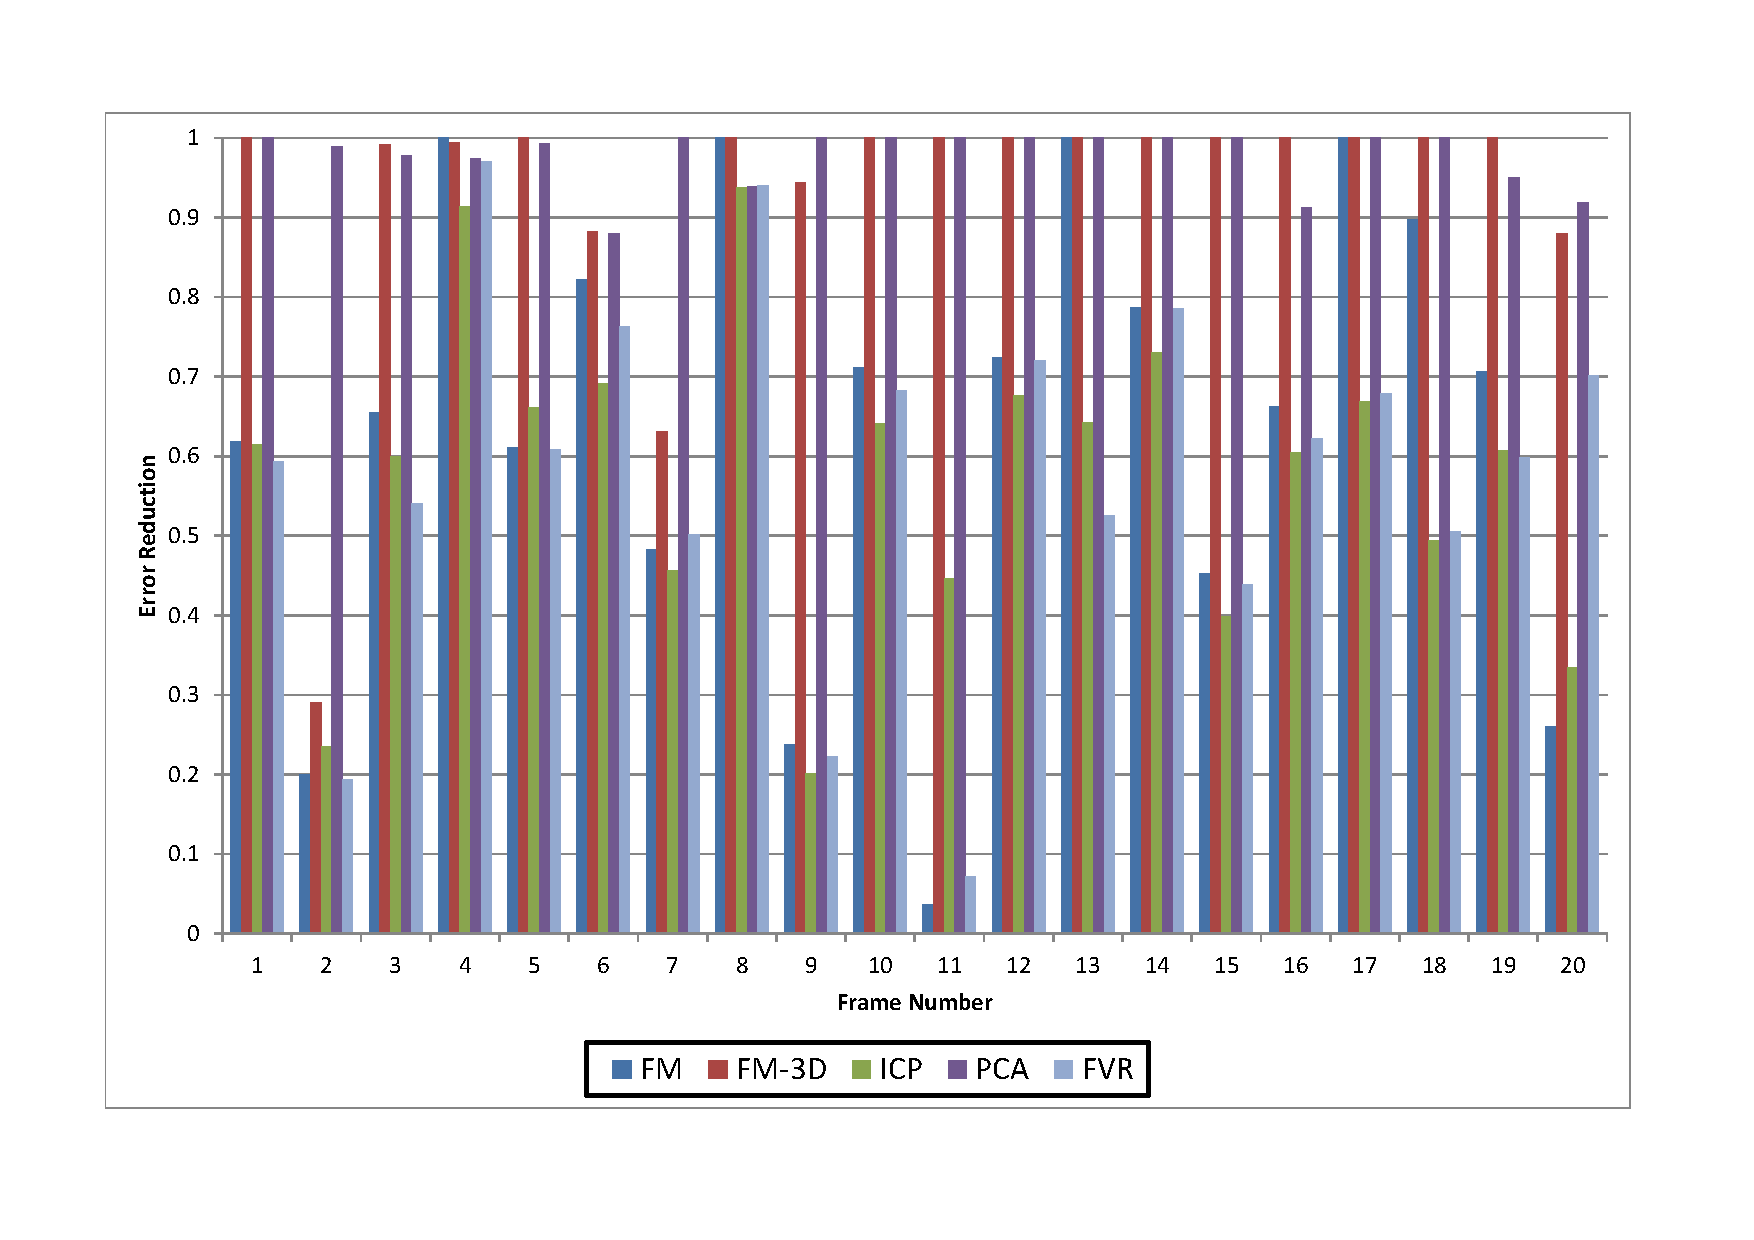
\includegraphics[width=6.0in]{images/results/Office_Texture_blind_spot_rotation}
\caption{Registration Error for the Office Centered Object Rotation Data Set}
\label{fig:PET9}
\end{figure*}

Figure \ref{fig:PET9} shows results for the centred object rotation scene. Here, a large divider was placed in the middle of two desks. The idea was to create an environment where the large divider could throw off the effects of PCA and FVR and give an advantage to the feature matching approaches and ICP. Interestingly, around 35\% of the time, FVR had the best result. 2D-feature-matching outperformed the 3D counterpart but only got the best result 10\% of the time. ICP on the other hand got the best result for around 55\% of the frames. It is suspected that ICP is able to use the large divider as an anchor which would make it more robust to non-overlapped data.

\begin{figure*}[t]
\centering
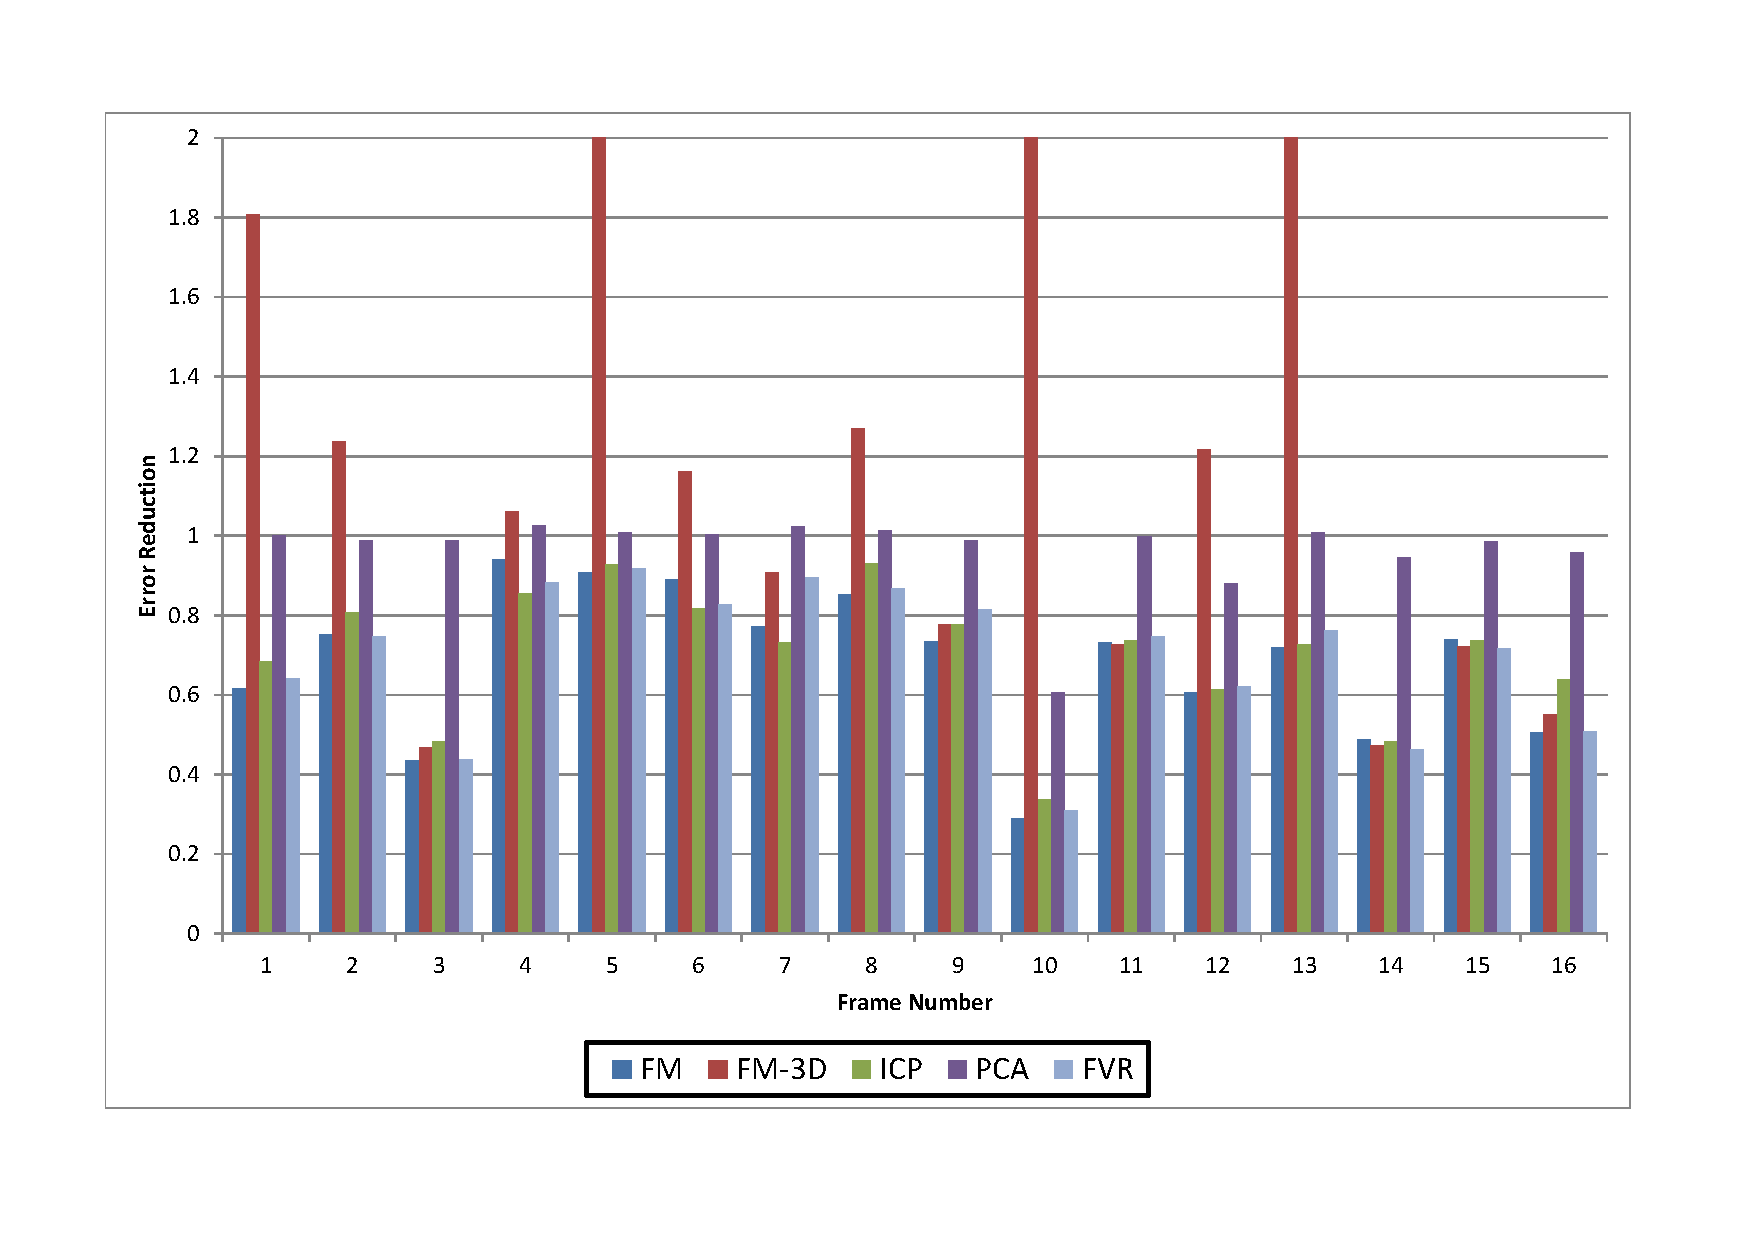
\includegraphics[width=6.0in]{images/results/Office_Texture_Rotate_XAxis}
\caption{Registration Error for the Office X/Y-Axis Rotation Data Set}
\label{fig:PET10}
\end{figure*}

Another experiment where the scene was filmed with the camera rotated predominantly about the x-axis is shown in figure \ref{fig:PET10}, this time 2D-feature-matching, ICP and FVR all performed similarly, with only PCA and 3D-feature-matching failing to get good registrations. 

\begin{figure*}[t]
\centering
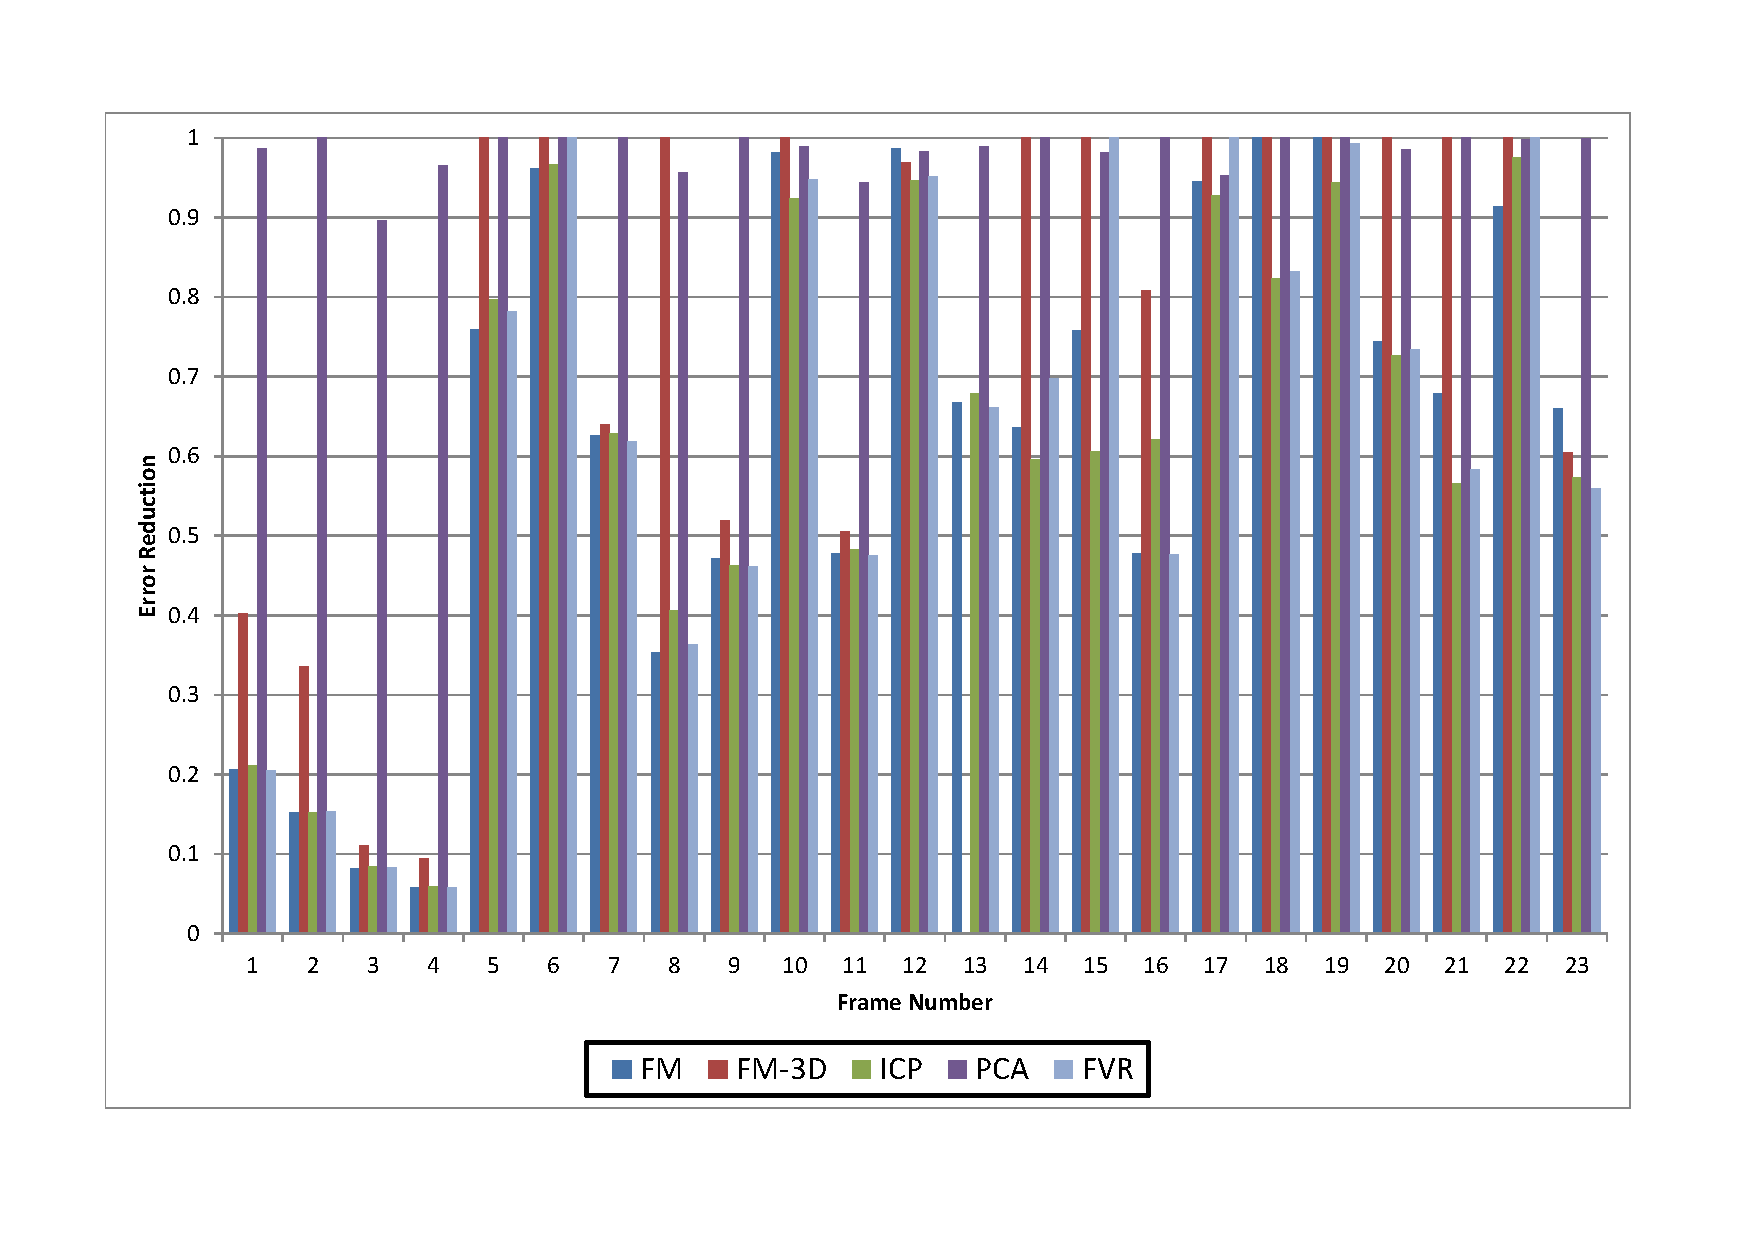
\includegraphics[width=6.0in]{images/results/Office_Texture_Rotation}
\caption{Registration Error for the Office Y-Axis Rotation Data Set}
\label{fig:PET11}
\end{figure*}

Figure \ref{fig:PET11} shows the registration errors for the Office data-set with camera rotation about the Y-axis. Here, in around 50\% of the cases, FVR outperformed or matched the best result. 2D-feature-matching was next best matching or outperforming the best result around 34\% of the time. Interestingly, PCA performed the worst with this data-set. Because rotation can incur a smaller overlap and thus a large shift in the axes and mean of the principal components, this could be expected.

\begin{figure*}[t]
\centering
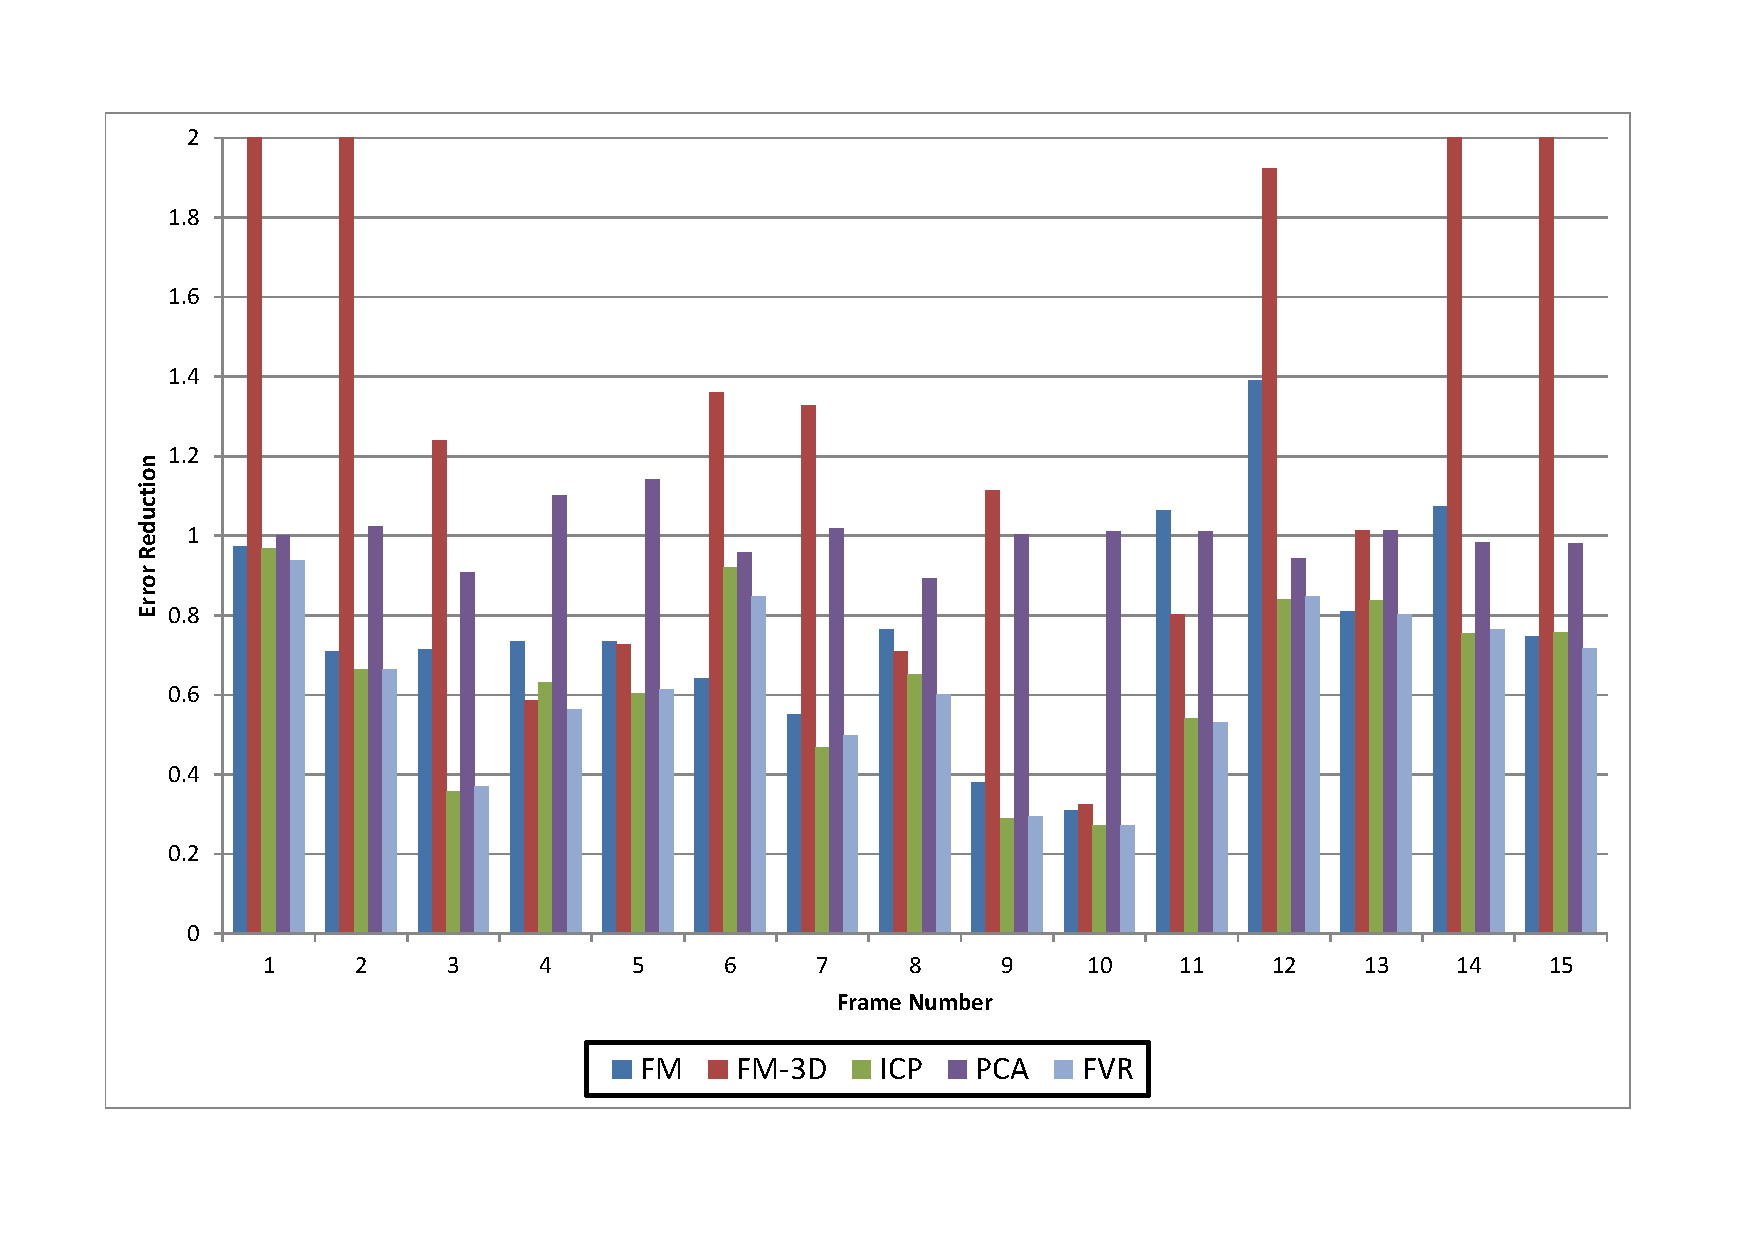
\includegraphics[width=6.0in]{images/results/Office_Texture_Translation}
\caption{Registration Error for the Office Translation Data Set}
\label{fig:PET12}
\end{figure*}

In the Office translation scene, FVR outperformed or matched the other algorithms around 85\% of the time. This shows that the FVR has high accuracy when dealing with translation detection and the registration of 3D data with only translational changes. Here, PCA and 3D-feature matching performed the worst with ICP and 2D-feature matching also being quite consistent and robust.

\begin{figure*}[t]
\centering
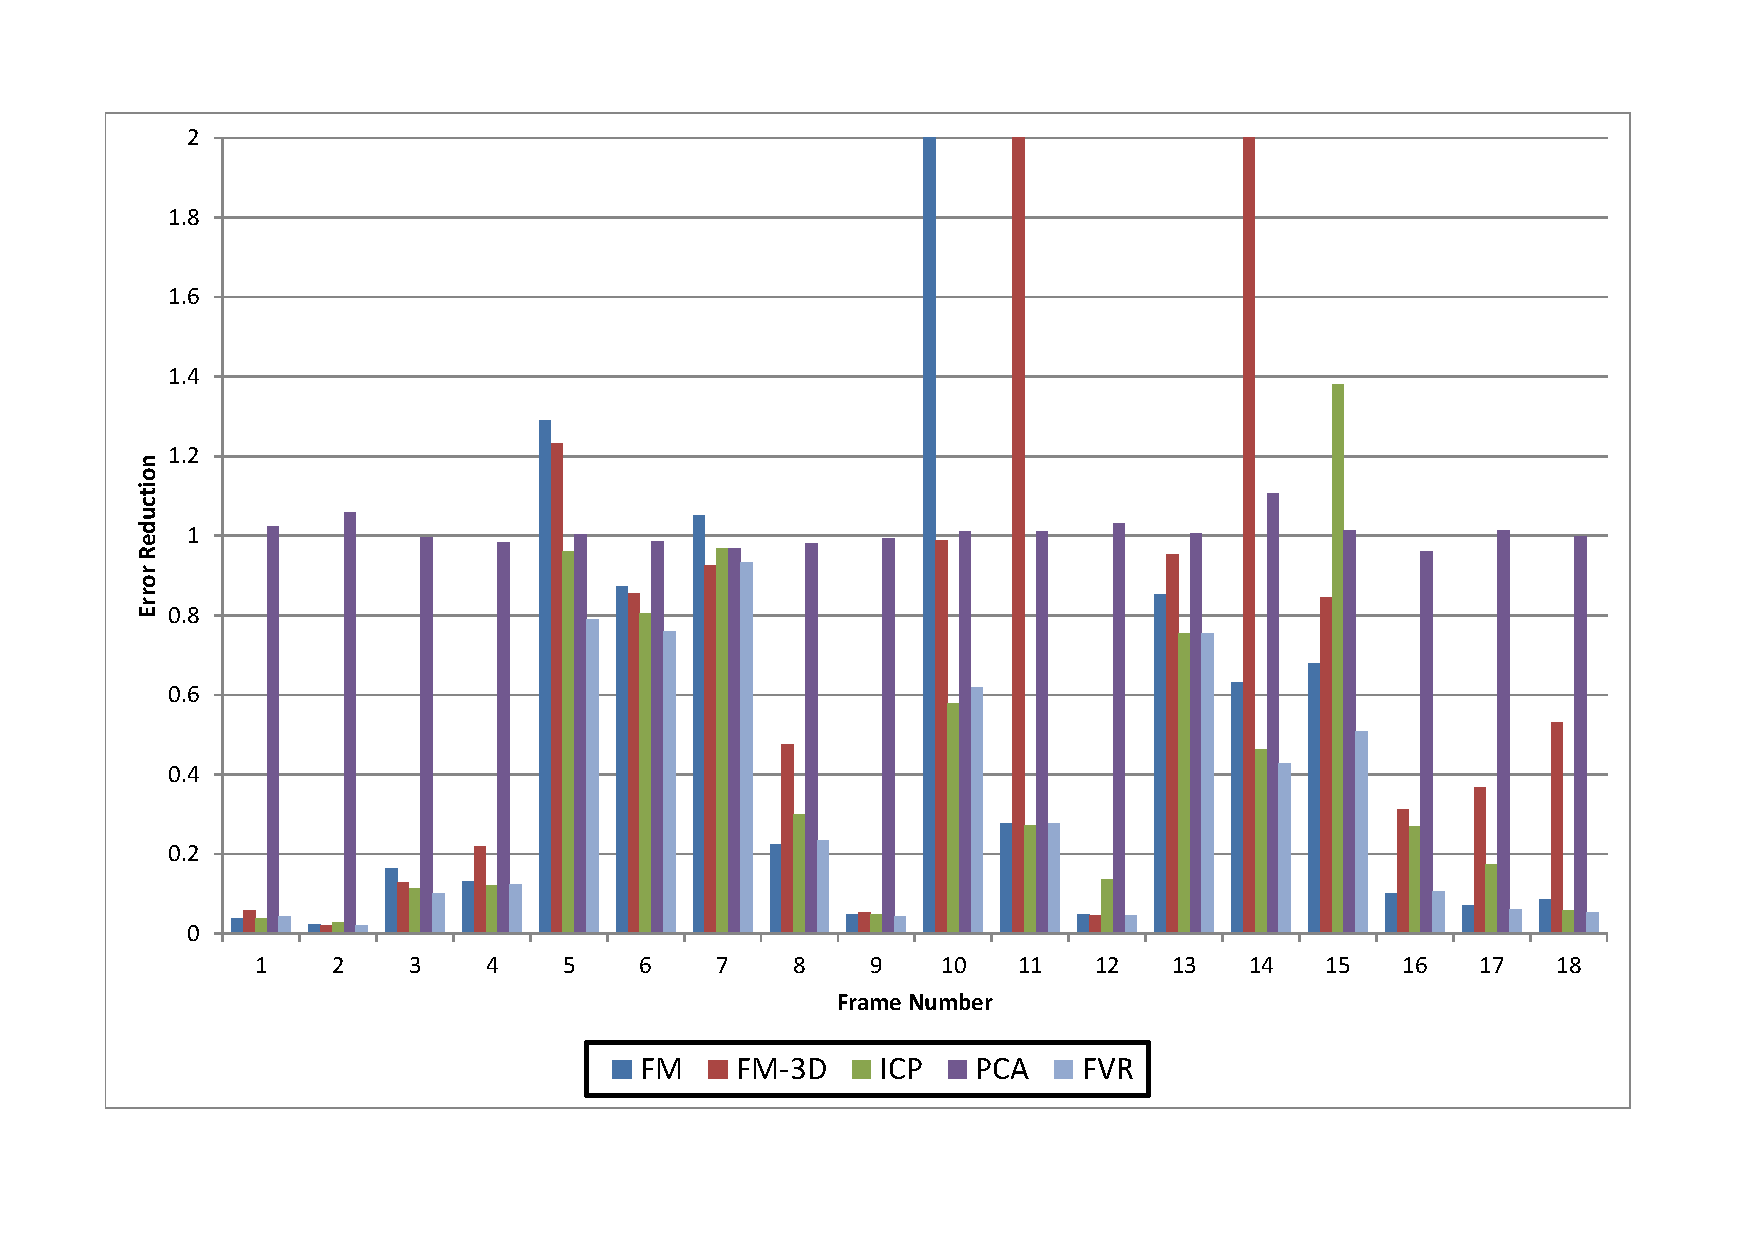
\includegraphics[width=6.0in]{images/results/Outside_No_Texture_Rotation}
\caption{Registration Error for the Little Texture Outdoors Rotation Data Set}
\label{fig:PET13}
\end{figure*}

Figure \ref{fig:PET13} shows results for an outdoors scene with little texture, here the camera was rotated about an origin. In this case, PCA performed the worst, and 3D-feature-matching also failed several times. The only algorithm which did not fail once was FVR. In this test, FVR outperformed or matched the other algorithms 88\% of the time. This can be explained by FVR's robustness to out-door scenes and scenes with little texture. 

\begin{figure*}[t]
\centering
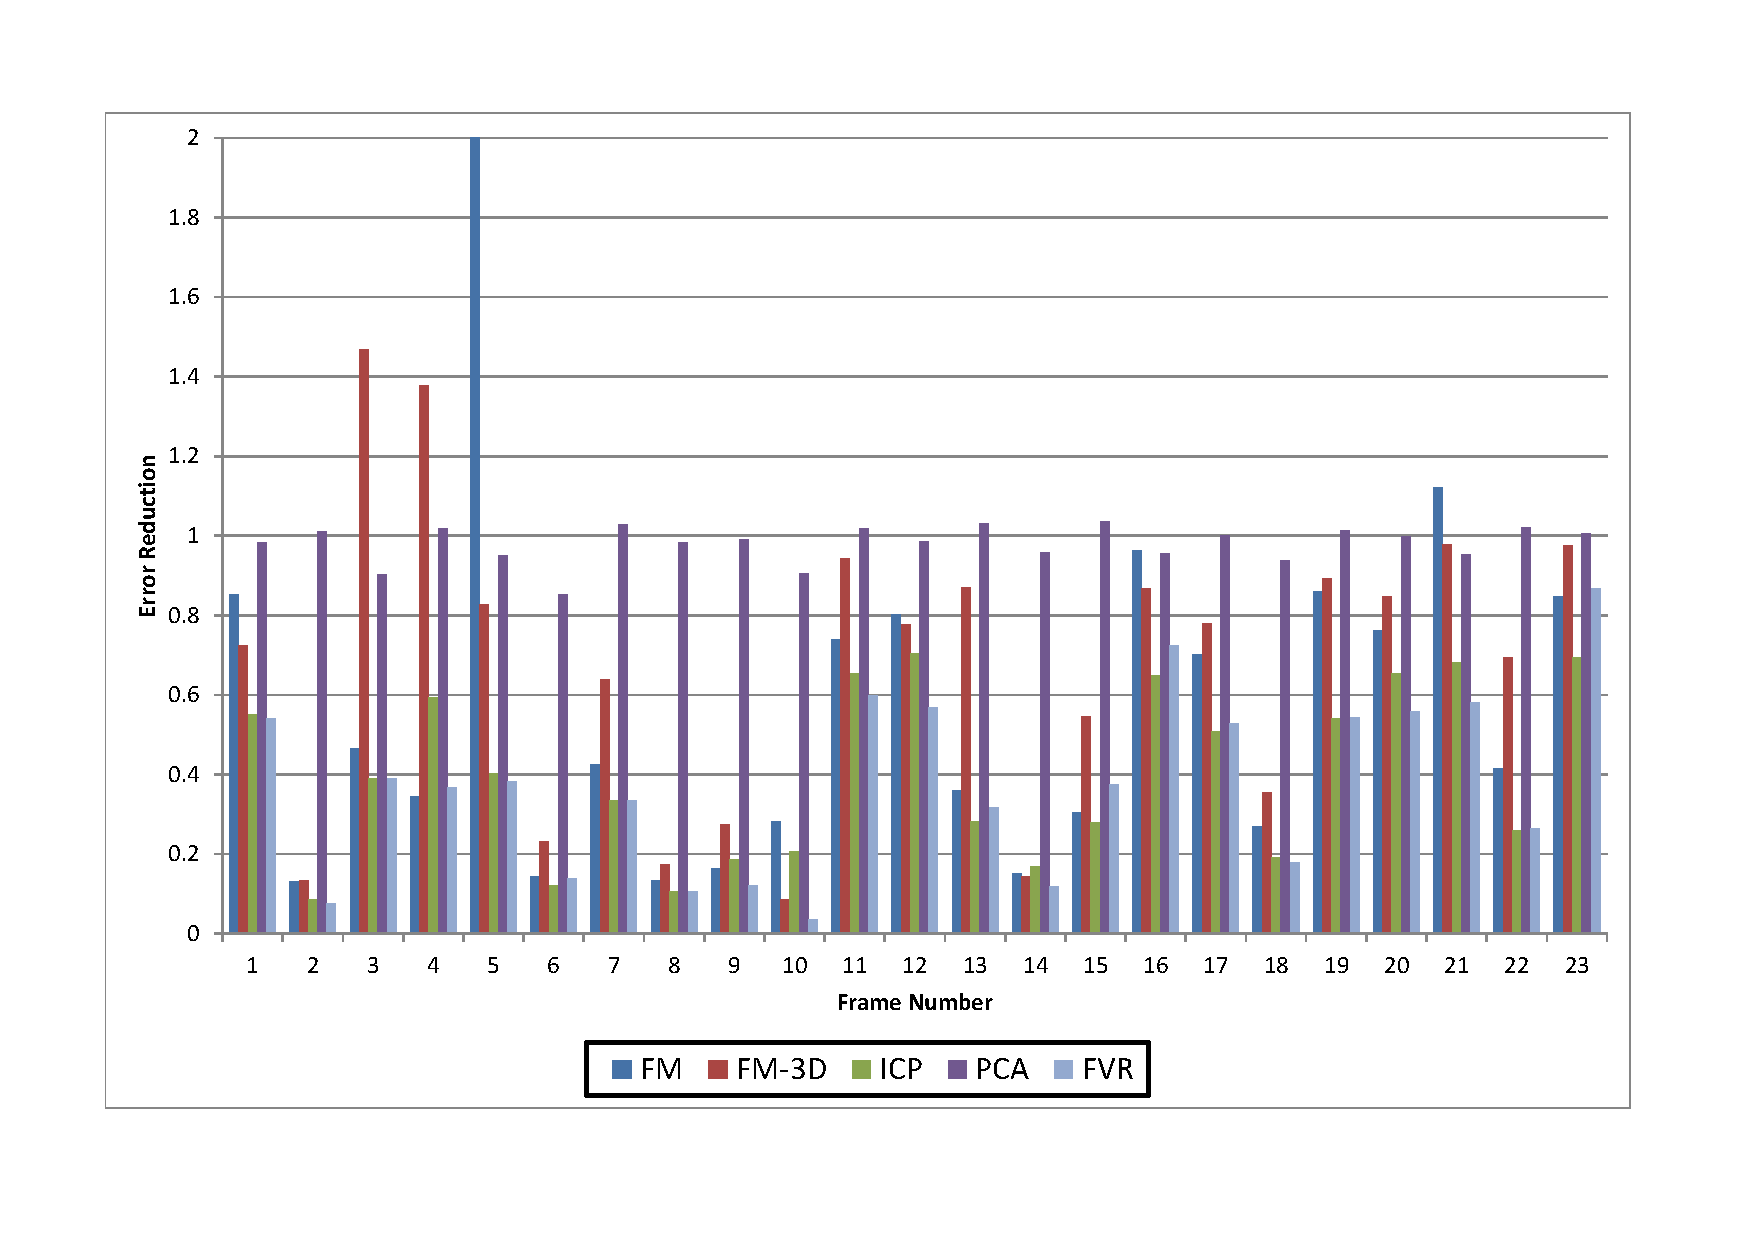
\includegraphics[width=6.0in]{images/results/Outside_No_Texture_Translation}
\caption{Registration Error for the Little Texture Outdoors Translation Data Set}
\label{fig:PET14}
\end{figure*}

Another test using a low-textured out-doors scene was tested where the camera was translated along a path. Results are shown in figure \ref{fig:PET14}. Here again the FVR method dominated recording either the best result or matching best result for around 73\% of the frames. Notably, PCA performed poorly, and both the feature-matching methods failed to register a few times. ICP was more consistent, recoding the best or equivalent result around 47\% of the time. Again, this shows the strength of the FVR method in out-door and low-texture environments. 

\begin{figure*}[t]
\centering
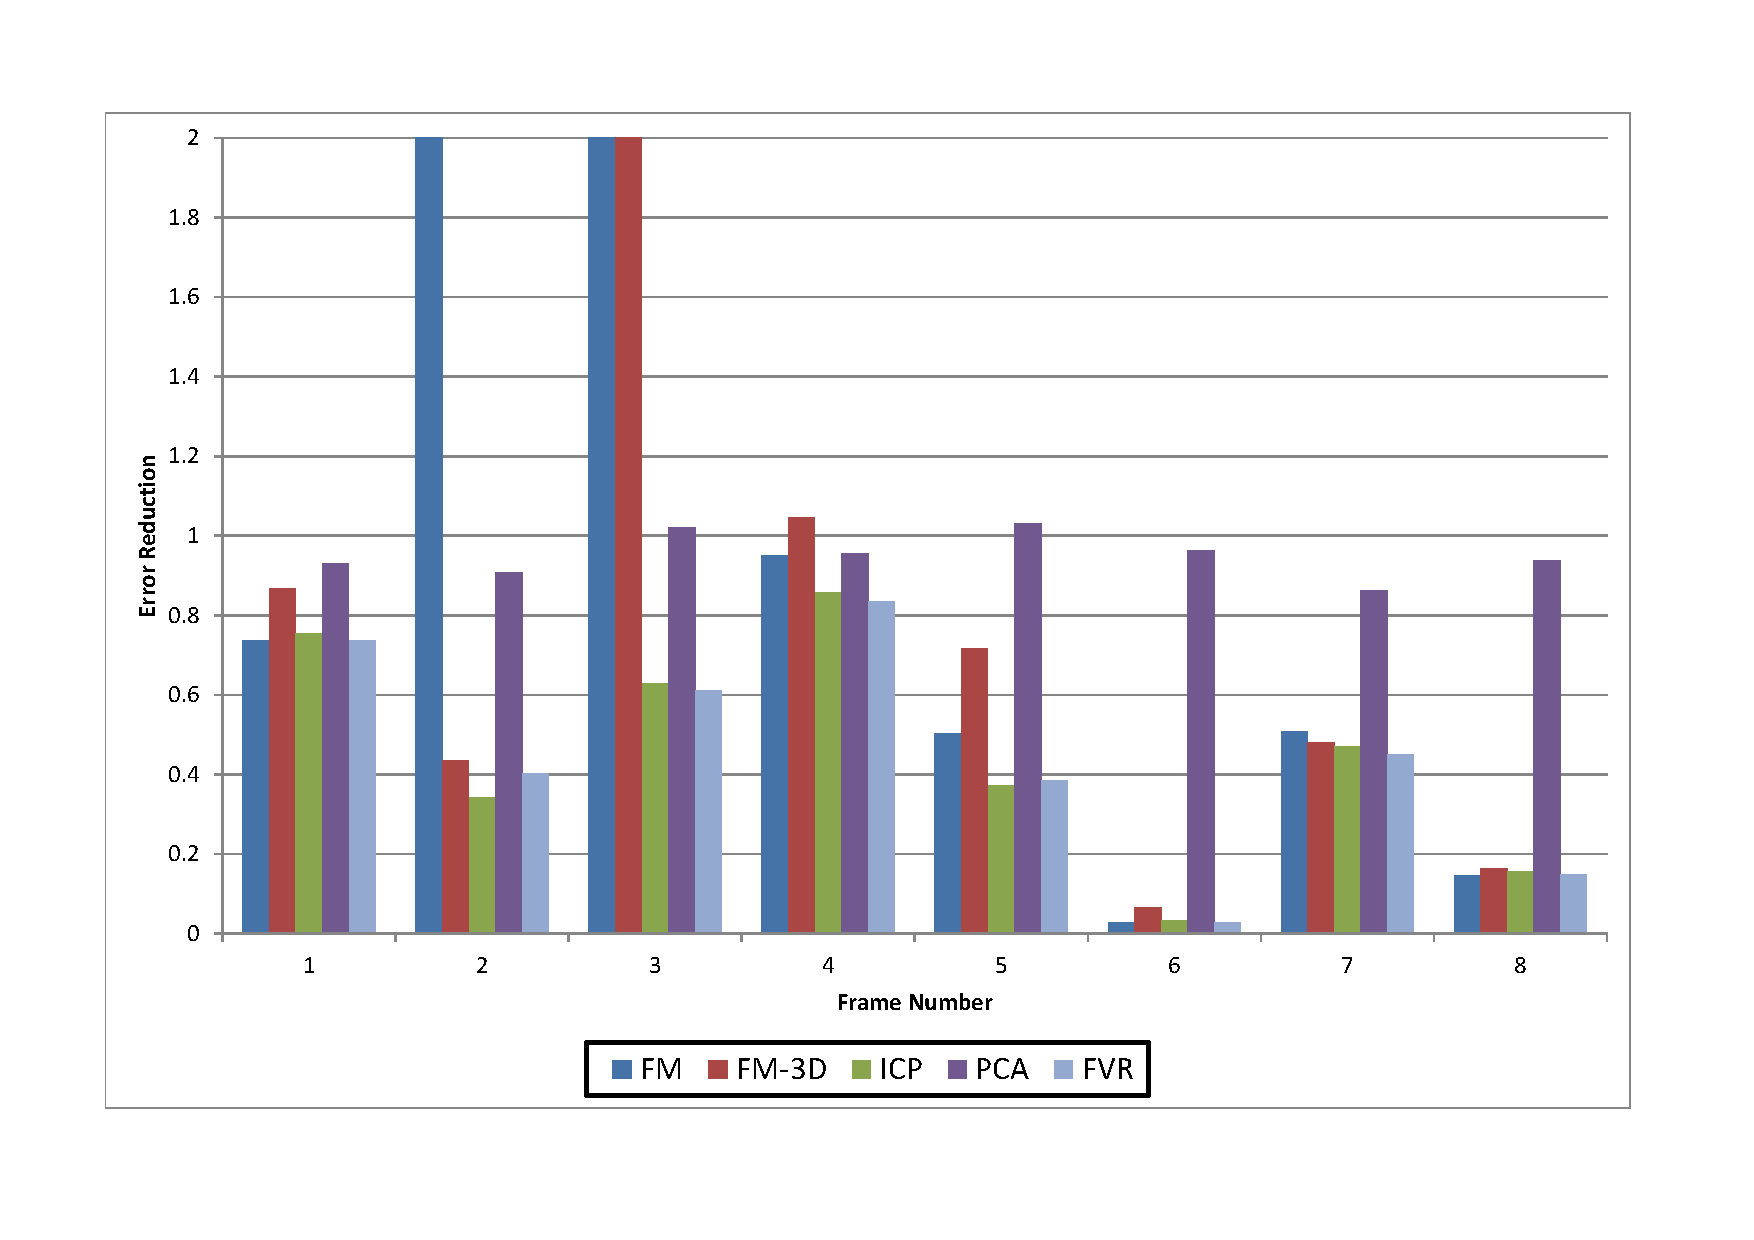
\includegraphics[width=6.0in]{images/results/Outside_TextureConfusion_Rotation}
\caption{Registration Error for the Outdoors Texture Confusion Rotation Data Set}
\label{fig:PET15}
\end{figure*}

Another test was performed with an outdoors scene. Here only 8 of the frames had any good results for all algorithms. They are shown in figure \ref{fig:PET15}. In these results, 6 out of the 8 frames had either a matching or best registration for the FVR method. 2D-feature-matching and 3D-feature-matching both failed a few times, and PCA was inconsistent. ICP had a competitive result 3 out of the 8 times, both FVR and ICP were most consistent. 

\begin{figure*}[t]
\centering
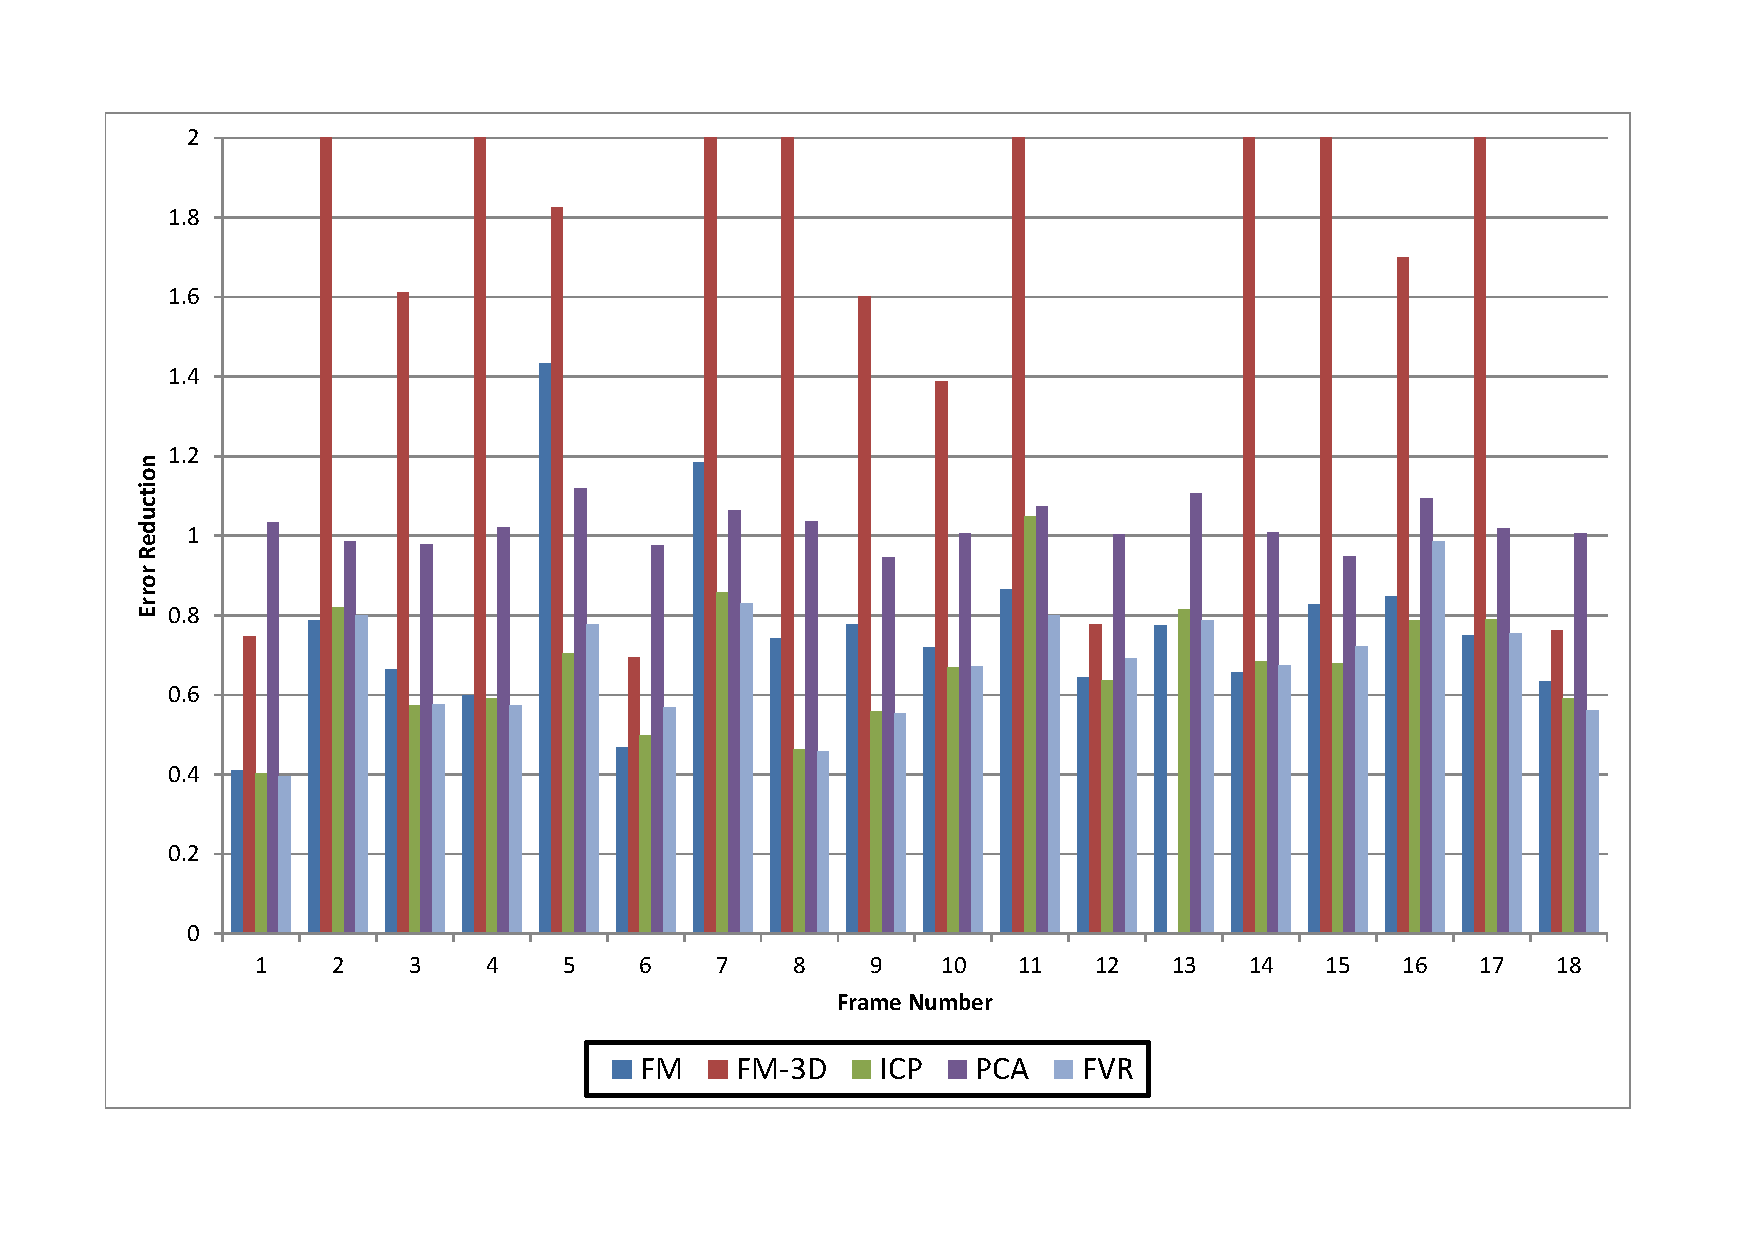
\includegraphics[width=6.0in]{images/results/Outside_TextureConfusion_Translation}
\caption{Registration Error for the Outdoors Texture Confusion Translation Data Set}
\label{fig:PET16}
\end{figure*}

Another scene with texture-confusion was taken out-doors. The interesting results are shown in figure \ref{fig:PET16}. Here, 3D-feature matching failed a majority of the time. Interestingly PCA also failed, the likely reason is because of the amount of noise in an out-doors scene. This noise can give inconsistencies in the principal axes and mean computation. Again, FVR performed best with it getting the best or equivalent result around 55\% of the time. This is another experiment where FVR is shown to be highly robust to scenes with texture confusion. 

\begin{figure*}[t]
\centering
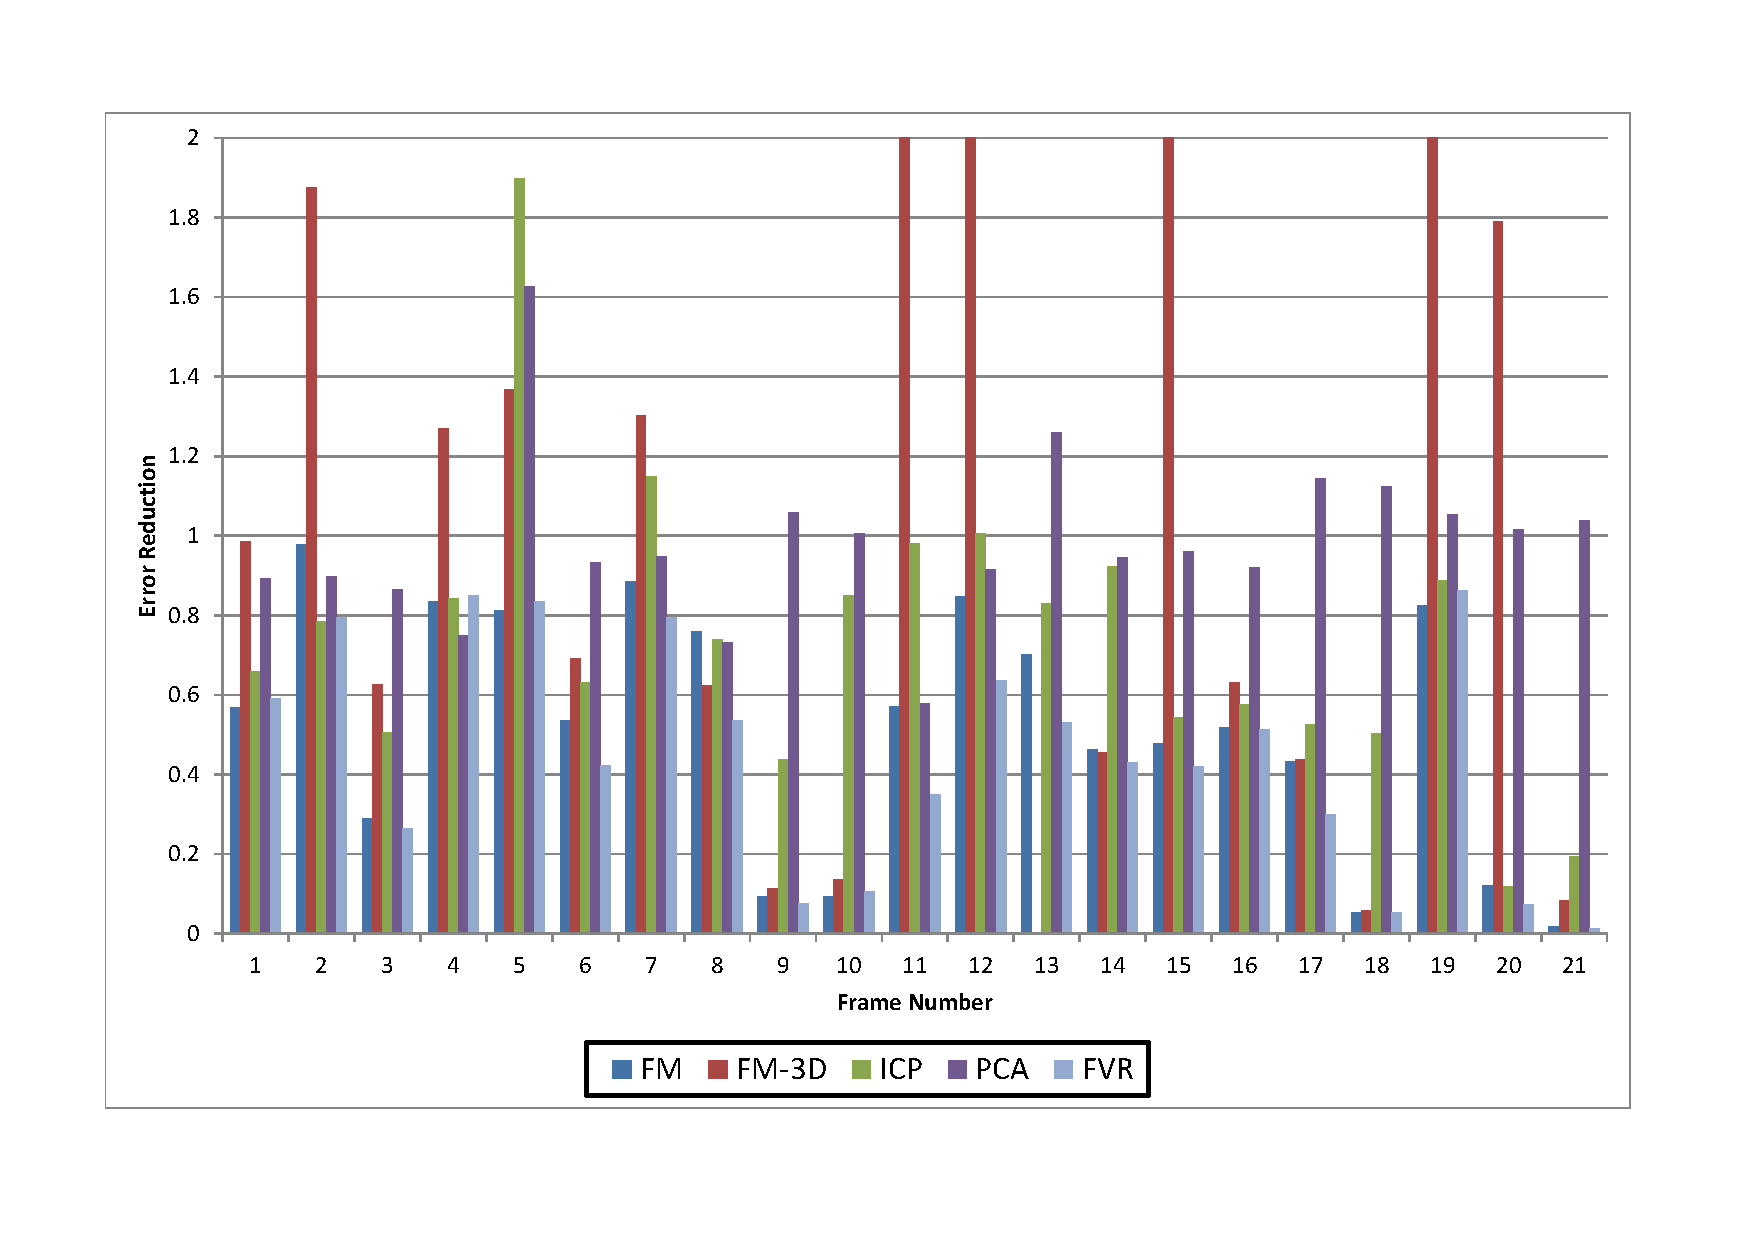
\includegraphics[width=6.0in]{images/results/Plants_Outdoors_Texture_Confusion_Rotation}
\caption{Registration Error for the Outdoor Plants Texture Confusion Rotation Data Set}
\label{fig:PET17}
\end{figure*}

The final figure in the pose estimation tests shows another scene taken out-doors. This scene also contains texture confusion, but the camera was rotated about an axis rather than translated in this data-set. Results shown in figure \ref{fig:PET17} indicate that again FVR dominates with 16 out of the 21 frames having a matching or best registration by FVR. 

\section{Plane-Tree: Qualitative Results}
\label{SEC:PTQUALEVAL}

\begin{figure*}[!htb] 
        \centering
 		\begin{subfigure}[b]{1.9in}
                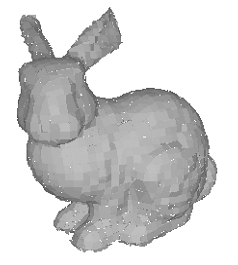
\includegraphics[width=1.6in]{images/results/compression/bunnyb}
                \caption{2.03 bpv\\8827 bytes}
                \label{fig:FIG_BUNNYB}
        \end{subfigure}%
        \begin{subfigure}[b]{1.9in}
                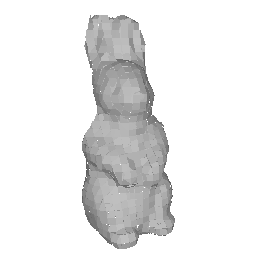
\includegraphics[width=1.6in]{images/results/compression/rabbitb}
                \caption{0.47\\3898 bytes}
                \label{fig:FIG_RABBITB}
        \end{subfigure}%
        \begin{subfigure}[b]{1.9in}
                \includegraphics[width=1.6in]{images/results/compression/horseb}
                \caption{1.55 bpv\\3842 bytes}
                \label{fig:FIG_HORSEB}
        \end{subfigure}

        \begin{subfigure}[b]{1.9in}
                \includegraphics[width=1.6in]{images/results/compression/bunnyd}
                \caption{7.74 bpv\\33701 bytes}
                \label{fig:FIG_BUNNYD}
        \end{subfigure}%
        \begin{subfigure}[b]{1.9in}
                \includegraphics[width=1.6in]{images/results/compression/rabbitd}
                \caption{1.97\\16492 bytes}
                \label{fig:FIG_RABBITD}
        \end{subfigure}%
        \begin{subfigure}[b]{1.9in}
                \includegraphics[width=1.6in]{images/results/compression/horsed}
                \caption{5.95 bpv\\14758 bytes}
                \label{fig:FIG_HORSED}
        \end{subfigure}
        
        \begin{subfigure}[b]{1.9in}
                \includegraphics[width=1.6in]{images/results/compression/bunnyorig}
                \caption{original: 518.78 bpv\\2,258,902 bytes}
                \label{fig:FIG_BUNNYO}
        \end{subfigure}%
        \begin{subfigure}[b]{1.9in}
                \includegraphics[width=1.6in]{images/results/compression/rabbitorig}
                \caption{original: 530.14\\4,442,413 bytes}
                \label{fig:FIG_RABBITO}
        \end{subfigure}%
        \begin{subfigure}[b]{1.9in}
                \includegraphics[width=1.6in]{images/results/compression/horseorig}
                \caption{original: 519.92 bpv\\1,290,120 bytes}
                \label{fig:FIG_HORSEO}
        \end{subfigure}
       
       \caption{Models coded with our coder at thresholds of 8.0 and 1.0 with a maximum tree depth of 6 along with the original models.}
       \label{fig:FIGS}
\end{figure*}

In Figure \ref{fig:FIGS} we present qualitative results for the Plane-Tree. The third row shows the bunny, rabbit and horse models along with the number of bytes and bpv required to store them uncompressed. The first row shows each model compressed by the Plane-Tree with a threshold of 8.0. Despite these being crude approximations of the originals, the models are still distinguishable with around 1000 $\times$ less storage space required. \\

In the second row, each model was compressed with the Plane-Tree at a threshold of 1.0. In these experiments, there is little detail missing compared with the physical model. When looking at the bunny's legs, the same ripples are present. In the rabbit model, the outlines inside the ears and on the eyes are still present. On the horse model, the creases on the body and shoulder of the horse are still present. Here, the bunny is compressed to around 70 $\times$ less storage space, the rabbit at around 265 $\times$ less and the horse around 90 $\times$ less storage space. \\


\begin{figure}[H] 
        \begin{center}
 		\begin{subfigure}[b]{3in}
 			   \centering
 			   \includegraphics[width=2.8in]{images/experiments/pt_qual/original1}
                \caption{Original\\518.78 bpv\\2,258,902 bytes}
                \label{fig:FIG_BUNNYB}
        \end{subfigure}%
        \begin{subfigure}[b]{3in}
                \includegraphics[width=2.8in]{images/experiments/pt_qual/planetree_shade}
                \caption{Plane-Tree\\3.88 bpv\\16,896 bytes}
                \label{fig:FIG_RABBITB}
        \end{subfigure}
        \begin{subfigure}[b]{3in}
                \includegraphics[width=2.8in]{images/experiments/pt_qual/tg}
                \caption{Touma and Gotsman \cite{touma98triangle}\\4.1 bpv\\17,852 bytes}
                \label{fig:FIG_HORSEB}
        \end{subfigure}%
        \begin{subfigure}[b]{3in}
                \includegraphics[width=2.8in]{images/experiments/pt_qual/kg}
                \caption{Karni and Gotsman \cite{Karni00Spectral}\\4.1 bpv\\17,852 bytes}
                \label{fig:FIG_BUNNYD}
        \end{subfigure}
       \caption{The Bunny Model Compressed Using the Plane-Tree, Karni and Gotsman and Touma and Gotsman.}
       \label{fig:qualSOTA1}
       \end{center}
\end{figure}


\begin{figure}[H] 
        \begin{center}
 		\begin{subfigure}[b]{2in}
 			   \centering
 			   \includegraphics[width=1.8in]{images/experiments/pt_qual/original2}
                \caption{Original\\518.78 bpv\\2,258,902 bytes}
                \label{fig:FIG_BUNNYB}
        \end{subfigure}%
        \begin{subfigure}[b]{2in}
                \includegraphics[width=1.8in]{images/experiments/pt_qual/planetree2_shade}
                \caption{Plane-Tree\\0.31 bpv\\1,349 bytes}
                \label{fig:FIG_RABBITB}
        \end{subfigure}%
        \begin{subfigure}[b]{2in}
                \includegraphics[width=1.8in]{images/experiments/pt_qual/khodakovsky_shade}
                \caption{Khodakovsky et al. \cite{Khodakovsky00Progressive}\\0.31 bpv\\1,349 bytes}
                \label{fig:FIG_HORSEB}
        \end{subfigure}
       \caption{The Bunny Model Compressed Using the Plane-Tree and Khodakovsky et al.}
       \label{fig:qualSOTA2}
       \end{center}
\end{figure}


\section{Plane-Tree: Reconstruction Compression}
\label{SEC:PTONRECON}

In this section, experiments comparing the Plane-Tree with the octree in terms of 3D frame or 3D occupancy reconstruction grid compression. Essentially this experiments compares the performance of the Plane-Tree and octree in 3D occupancy grid compression. \\

The octree is used for comparison since it is the closest relative of the Plane-Tree and existing methods which use the octree are presently used in 3D reconstruction research. There is also a 3D implementation of the Interpolating Leaf Quad-Tree \cite{Lincoln13Interpolating} compression algorithm used in the comparison. Being the 3D extension, it is therefore referred to as the Interpolating Leaf octree algorithm (ILOT). \\

In this experiment, Rate-Distortion is measured in PSNR (Peak Signal to Noise Ratio) which is a measurement of the amount of accuracy between the original model and the compressed version for a given algorithm and level of compression. The larger the PSNR, the higher the quality in which the compression system produces for a given bitrate. \\

A Rate-Distortion graph comparing the Plane-Tree, octree and ILOT is presented in Figure \ref{fig:3DReconCompression1}. Results show that for low bit-rates the ILOT outperforms the octree method. However as higher quality is required, the octree in turn outperforms the ILOT method. The Plane-Tree algorithm proposed in this work is shown to be dominant compared to both algorithms. For each algorithm, at any bitrate, the Plane-Tree has a much larger Peak-Signal-To-Noise ratio. \\

\begin{figure}[!htb]
\centering
\includegraphics[width=4.0in]{images/results/compression/psnr1}
\caption{PSNR vs Bitrate comparing the ILOT, OT and PT compression methods.}
\label{fig:3DReconCompression1}
\end{figure}

In conclusion, as in results comparing the Plane-Tree with state-of-the-art mesh compression algorithms, the Plane-Tree is shown to perform well and even outperform ILOT and the generic octree data structures when compressing 3D data used in reconstructions. 




